% Page settings
\documentclass[notitlepage,12pt]{article}
\usepackage{fancyvrb, verbatim, listings}                                  % Various for inserting/hosting code
\usepackage{setspace}                                                      % Space between lines (customisable)
\usepackage[margin=2.54cm]{geometry}                                       % Set margins (standard is 2.54cm)
\usepackage[UKenglish,cleanlook]{isodate}                                  % Set default date and date display
\usepackage{fancyhdr} \pagestyle{fancy}                                    % Line the top of the page
\usepackage[activate={true,nocompatibility},final,tracking=true,kerning=true,spacing=true,factor=1100,stretch=10,shrink=10]{microtype}
\microtypecontext{spacing=nonfrench}                                       % Change font and minor spacings to look nicer
\setlength{\parskip}{0.5\baselineskip}                                     % Set default paragraph behaviour: skip a line
%\setlength{\parindent}{0pt}                                                % Set default paragraph behaviour: no indent
%% Packages to use:
% Tables + figures
\usepackage{graphicx}                                                      % control over the import of graphics
\usepackage[table,dvipsnames]{xcolor}                                      % Define tables (with colour control)
\usepackage{float}                                                         % Control over graphics + tables float
\usepackage[justify]{ragged2e}                                             % control over text alignment
\usepackage{booktabs}                                                      % caption graphics + tables (with name in bold)
\usepackage[labelfont=bf]{caption} 
\usepackage{subcaption}
% caption graphics + tables (with name in bold)
\usepackage{tikz}                                                          % Draw graphs inline, guide: https://sites.google.com/site/kochiuyu/Tikz
\usetikzlibrary{shapes,decorations,arrows,calc,arrows.meta,fit,positioning}
\tikzset{
    -Latex,auto,node distance =1 cm and 1 cm,semithick,
    state/.style ={ellipse, draw, minimum width = 0.7 cm},
    point/.style = {circle, draw, inner sep=0.04cm,fill,node contents={}},
    bidirected/.style={Latex-Latex,dashed},
    el/.style = {inner sep=2pt, align=left, sloped}
}
\usepackage{pgfplots} \pgfplotsset{compat=1.16}                            % Automatic graphing, read https://www.overleaf.com/learn/latex/pgfplots_package for examples
% Maths + numbers
\usepackage{mathtools}                                                     % Various maths functions
\usepackage{amssymb}                                                       % Various maths functions
\usepackage{amsmath}                                                       % Various maths functions
\usepackage{dsfont}                                                        % Various maths functions
\usepackage{centernot}                                                     % center \not usage
\usepackage{siunitx} \sisetup{round-mode=places, round-precision=3}        % Formalise use of units and numbers among text
\DeclareMathOperator{\eps}{\varepsilon}                                    % epsilon short hand shortcut
\DeclareMathOperator{\st}{\text{ s.t. }}                                   % "such that" short hand shortcut
\DeclareMathOperator{\then}{\text{ then }}                                 % "then" in equation shortcut
\DeclareMathOperator{\ifeq}{\text{ if }}                                   % "if" in equation shortcut
\DeclareMathOperator{\oreq}{\text{ or }}                                   % "or" in equation shortcut
\DeclareMathOperator{\andeq}{\text{ and }}                                 % "and" in equation shortcut
\DeclareMathOperator{\all}{,\; \forall}                                    % all (with spacing) in equation shortcut
\DeclareMathOperator{\N}{\mathbb{N}}                                       % N, natural number, shortcut
\DeclareMathOperator{\R}{\mathbb{R}}                                       % R, real number, shortcut
\DeclareMathOperator{\Ll}{\mathcal{L}}                                     % L, Lagrangian, shortcut
\renewcommand{\vec}[1]{\boldsymbol{\mathit{#1}}}                           % vector notation shortcut
\newcommand{\mat}[1]{\boldsymbol{\mathit{#1}}}                             % matrix notation shortcut
\DeclarePairedDelimiter\abs{\lvert}{\rvert}                                % absolute value notation shortcut
\DeclarePairedDelimiter\norm{\lVert}{\rVert}                               % norm notation shortcut
\newcommand{\Prob}[1]{\Pr\left( #1 \right)}                         % SHortcut for probability notation
\newcommand{\Probgiven}[2]{\Pr\left( #1 \, \middle\vert \, #2 \right)} % SHortcut for probability notation, given
\newcommand{\E}[2][]{\mathbb{E}_{#1} \left[ #2 \right]}                    % Expectation (with optional subscript) shortcut
\newcommand{\Egiven}[3][]{\mathbb{E}_{#1} \left[ #2 \, \middle\vert \, #3 \right]} % Expectation given (with optional subscript) shortcut
\newcommand{\Var}[2][]{\text{Var}_{#1} \left( #2 \right)}                  % Variation (with optional subscript) shortcut
\newcommand{\Cov}[1]{\text{Cov} \left( #1 \right)}                         % Covariance (with optional subscript) shortcut
\newcommand{\median}[1]{\text{median} \left( #1 \right)}                   % Median (with optional subscript) shortcut
\newcommand{\indicator}[1]{\mathds{1}\left\{ #1 \right\}}                  % SHortcut for indicator function
\newcommand{\diff}[2][]{\frac{d#1}{d#2}}                                   % SHortcut for differential fraction as a function
\newcommand{\partialdiff}[2][]{\frac{\partial#1}{\partial#2}}              % SHortcut for partial differential fraction as a function
\newcommand{\converge}[1]{\xrightarrow{ #1 \to\infty}}                     % SHortcut for convergence arrow
\renewcommand{\hat}[1]{\widehat{#1}}                                       % Default estimator notation is widehat
\renewcommand{\bar}[1]{\overline{#1}}                                      % Make over bar look nicer
\renewcommand{\tilde}[1]{\widetilde{#1}}                                   % Make over tilde look better
% Citations
\usepackage[longnamesfirst]{natbib}                                        % Citation package, see https://en.wikibooks.org/wiki/LaTeX/Bibliography_Management#Natbib
\usepackage[backref=page]{hyperref}                                        % Allow for links across the text, with colour options
\hypersetup{colorlinks=true, linkcolor=blue, citecolor=blue, filecolor=magenta, urlcolor=blue}
\def\sectionautorefname~#1\null{Section~#1\null}                       % Fix autoref for sections
\def\equationautorefname~#1\null{Equation~(#1)\null}                       % Fix autoref for equations
% IMPORTANT: follow style guide here https://github.com/Wookai/paper-tips-and-tricks


%%%%%%%%%%%%%%%%%%%%%%%%%%%%%%%%%%%%%%%%
%% Title page
% Author
\author{Senan Hogan-Hennessy\thanks{
        For helpful comments I thank
        Levon Barseghyan,
        Francine Blau,
        Ryan Dycus,
        Ronald Ehrenberg,
        Michael Lovenheim,
        Jake Meyer,
        Douglas Miller,
        and Evan Riehl.
        I thank seminar participants at Cornell University (2022, 2023) for helpful discussion.
        This project's repository, with all materials and anonymised data needed for replication, is available at 
        \url{https://github.com/shoganhennessy/state-funding-faculty}.
        Any comments or suggestions may be sent to me at \href{mailto:seh325@cornell.edu}{\nolinkurl{seh325@cornell.edu}}, or raised as an issue on the Github project.
    } \\
    \vspace{0.1cm}
    Economics Department, Cornell University\footnote{
        Address: Uris Hall \#447, Economics Department, Cornell University NY 14853 USA.
    }
}
% Title
\title{Less Funding, More Lecturers, and Fewer Professors: \\ \vspace{0.1cm}
    \Large{Stagnating State Funding for Higher Education and its Effect on Faculty at Public Universities}}
\date{This version: \today \\ \vspace{0.1cm}
    \href{https://github.com/shoganhennessy/state-funding-faculty/blob/main/state-funding-faculty-2023.pdf}{Newest version available here.}
}
\rhead{\today}
\lhead{Less Funding, More Lecturers, and Fewer Professors.}
% Begin
\begin{document}
\maketitle
\thispagestyle{empty}
% Abstract
\begin{abstract}
    \noindent
    Public universities employ more lecturers and fewer professors than at any other point in the last thirty years, relative to student enrolment.
At the same time, state funding for higher education has stagnated.
This paper shows that the decline in state funding led to a substitution away from professors toward lecturers at US public universities.
Using a shift-share approach to instrument for state funding, I find that universities employ 4.4\% more lecturers per student following a 10\% funding cut.
This shift is accompanied by a reduction in assistant professors and full professors per student by 1.4\% and 1.2\%, respectively.
Incumbent professors' salaries, promotion rates, and quit rates at Illinois universities remain unaffected by funding cuts, indicating that the substitution arose from limiting the hiring of new tenure-track/tenured professors.
Stagnating state funding impacts public universities and faculty, likely contributing to the deterioration of student outcomes at public universities since the 1990s.

\vfill
\noindent
\textbf{Key-words:}
Faculty,
Higher Education,
State Funding

\vspace{0.05cm}
\noindent
\textbf{JEL Codes:} H72, I22, J45

\end{abstract}

%%%%%%%%%%%%%%%%%%%%%%%%%%%%%%%%%%%%%%%%%
%% Starting the paper
\newpage
\setcounter{page}{1}
\doublespacing
% Introduction section
\noindent
Public universities educate the majority of higher education students in the US, yet have experienced a stagnation in state funding over the last three decades .
At the same time, public university employment of lecturers dramatically increased at public universities, while enrolment rose dramatically.
Previous research has examined the effects of the decline in state funding on student outcomes \citep{NBERw23736,NBERw27885}, but there is little evidence of the effects of this funding decline on faculty.
I show that four-year, degree-granting public universities have experienced a systematic decline in state funding per student, and use a shift-share instrument to show that this fall led to a substitution away from tenure-track/tenured professors towards contingent lecturers.
Analysis of all public university faculty in the state of Illinois shows that incumbent faculty were relatively unaffected, in terms of wages, promotion and quit rates, implying that changes in faculty composition arose by disrupting public universities' ability to hire or replace their tenure-track/tenured faculty. 
Private universities were not exposed to similar financial constraints during this same time period, and do not exhibit the substitution away from tenure-track/tenured professors, so that the stagnating state funding for public universities has implications for the wider structure of US higher education and research.

There are various margins through which funding cuts can impact a university's faculty.
A university's level of resources affect the ability that departments can hire new professors, retain their current faculty, or provide retirement incentives, so it is natural to expect that funding cuts may affect the composition of professors at a university.
Similarly, the wages a university pays their faculty is affected by funding for the university, including the starting salary it offers to new professors and the amount of yearly raises (if any) for incumbent faculty.
So that it is natural to expect that systematic funding cuts will lead to changes in faculty composition, and possibly affect incumbent professors, too.
Yet, it is a priori unclear whether/how much each of these margins adjusts to funding cuts, as these decision depend on how the university administrations view the productivity of different inputs, plus the degree of wage and employment stickiness over time.

US universities are widely considered the highest performing in the world, yet there are consequential differences between its universities that operate in the private sector and those established by state governments.
Public universities are subject to numerous state-level administrative laws, and rely on their state governments for funding: an average public university received around \$11,600 of state funding per student in 1990, and only \$8,300 in 2021.
This fall is driven by a stagnation in the absolute level of state funding for higher education in most states, combined with a large increase of 46\% in student enrolment at public universities over the same time period.
Similarly, the number of lecturers per student over doubled, while the number of tenure-track/tenured professors per students fell by $-23$\% from 1990 to 2021.

I use data from the \cite{ipeds} to study the impact of changes in state funding for US public universities 1990--2017.
I combine these data with panel data for every faculty member at Illinois public universities for 2010--2021 \citep{ibhed}, to measure how incumbent faculty (i.e., those already employed at the university) are affected by changes in state funding.
These data allow me to answer the following research question: if a US public university receives an extra \$1,000 for each of their students (or a 10\% increase), do they change the composition of faculty they employ?
If so, which positions do universities substitute away from, or towards, and do these funding cuts affect the faculty members themselves?

I employ a shift-share instrument to identify changes in state funding for higher education, which exploits how universities differ in their financial reliance on state funding, combined with yearly shocks to the amount an entire state funds higher education --- following \cite{NBERw23736,NBERw27885}.
State governments decide how to fund higher education by a complicated process which can be influenced by local economic conditions, changing state priorities, or even lobbying from the state universities themselves.
As such, state funding is not randomly assigned to universities and so it is necessary to employ an identification strategy, such as the shift-share instrument, to account for this.
The shift-share instrument interacts how much a university relies on state funding as a percent of revenues in a base period with the entire state's total funding per higher education student for each year, exploiting changes in funding and how much each university historically relied on state funding for higher education.
Additionally, I estimate effect of state funding on faculty multiple years after the initial funding cuts, using the local projections method thanks to the presence of time-series confounding between the funding shock and later years' level of state funding.\footnote{
    To the best of my knowledge, this is also the first paper to use the local projections method for a shift-share instrument.
    %Previous work ignored the potential time-series confoduning, and estimated linear instrumental variables.
}

Falls in state funding affect faculty composition at public universities, which substitute away from tenured and tenure-track professors towards contingent lecturers.
A funding cut of \$1,000 per student leads to an average university employing 6 more lecturers;
in percentage terms, a funding cut of 10\% per student leads to a fall of 1.4\% in the number of assistant professors per student at a university, a fall of 1.2\% for tenured professors, and an increase in 4.4\% the number of lecturers per student.
Local projection estimates show that these effects linger for three to four years after the initial funding shock, showing that the effect is not isolated to the year of the funding shock. 
Over the same time period, state funding per student fell by around 35\%, count of (tenure-tack/tenured) professors per student fell by 9\%, and lecturers per student increased by 99\%, so that these results show that falls in state funding explain around 53\% of the fall in professors per student
% i.e. -(35 * 0.137) / -9
and 15.5\% of the rise in lecturers per student.
% ie., (35 * 0.437) / 99
Additionally, I use individual level data on all Illinois public university professors in 2010-2021 to investigate whether the shocks to state funding affected individual professors.
Incumbent professors were not meaningfully affected, in terms of total salary, promotion rate, or rate of leaving the Illinois public university system.
Yet the hiring rate for new professors at public universities was negatively impacted by the falls in state funding (and by the funding shocks).
This implies that faculty composition change arose by limiting the hiring of new professors; public universities increasingly hired contingent lecturers, and increasingly did not replace their retiring (or leaving) professors.

Mine is the first paper to provide causal evidence on the impact of state funding on faculty composition, and wages.
The closest related research on higher education funding has examined how university spending affected graduation rates and levels of student debt \citep{NBERw23736,NBERw27885}, and university finances \citep{miller2022making,bound2019public,brown2014endowment}.
For faculty outcomes, multiple theoretically model university decision-making and faculty hiring (see e.g., \citealt{abe2015implications,johnson2009jep,NBERc13879}), while others measured how faculty at universities were affected by endowment shocks and the 2008 recession \citep{brown2014endowment,turner2014impact}.
These papers measure effects of funding and changes in university revenues, but do not measure effects on faculty, or other outcomes related to university instruction.

My results provide suggestive evidence on mechanisms for the previous research connecting state funding cuts for higher education and worsening student outcomes.
Substitution towards lecturers is likely a cost-cutting measure for funding constrained universities, though relying on these faculty --- who are often over-worked and not granted long-term employment protections --- may lead to worse student outcomes \citep{ehrenberg2005tenured,zhu2021limited,jaeger2011examining}.
Lastly, my results provide evidence that the long term trends in higher education funding are causally related, contributing to the literature in the long run trends in faculty outcomes \citep{ehrenberg2003studying} and trends in US higher education and funding \citep{hoxby2009changing}.

This paper proceeds as follows.
\autoref{sec:data} describes the data for university finances and faculty in Illinois, and trends in public university funding for the last three decades.
\autoref{sec:conceptual} gives the conceptual framework for how state funding may affect faculty.
\autoref{sec:empirics} draws the empirical framework for isolating the causal effects of state funding on faculty composition and individual faculty, and \autoref{sec:results} presents the empirical results.
\autoref{sec:discussion} discusses the context and implications for the findings.
\autoref{sec:conclusion} concludes.

% Data section
%%%%%%%%%%%%%%%%%%%%%%%%%%%%%%%%%%%%%%%%%
%% Data section
\section{Data and Institutional Context}
\label{sec:data}

\subsection{Data Description}
The data used in this analysis come from two primary sources: \citet[IPEDS]{ipeds} regarding institutional information including finances and enrolment, and \citet[IBHED]{ibhed} for data on every professor in the Illinois public university system.

IPEDS is a survey of higher educational institutions in the US, and legally requires institutions to participate in order to receive Federal Title IV student aid.\footnote{
    This statement means that IPEDS does not necessarily cover the universe of US higher education institutions, yet in practice every public university and not for-profit four-year institution is represented.
}
Data are consistent between the years 1990 and 2021,\footnote{
    The years 1987-1989 are represented in these data in an incompletion fashion, so I focus on the years 1990 onwards.
    Year refers to the calendar year of the spring term --- i.e., 1987 refers to the academic year that ran August 1986 to July 1987.
}
and provide information on the total revenues a university received from every source (including state governments), enrolment, plus faculty count and total expenditures on salaries.\footnote{
    I combine the Urban Institute's 2018 compilation of IPEDS data for the years 1990--2017, and manually combine raw NCES data on 2018-2021 for all relevant variables.
    Figures for enrolment, faculty counts and salaries come from the raw NCES version of IPEDS for all years, addressing inconsistencies in the Urban Institute's data formulation for these variables.
}
I restrict analysis to public, four-year, degree-granting institutions, as these institutions adhere to a standardised concept of faculty profile, where tenure and title of appointment (lecturer, assistant professor, etc.) are relatively standardised.
For-profit institutions employ and enrol a negligible share of professors and students respectively, while students at two-year institutions by majority intend to eventually enrol at a four-year institution \citep{mountjoy2022}, so that these institutions are not considered.

IPEDS reports the count of professors employed by position, as well as total salary expenditures by position.
This gives a resulting panel data-set, where each row represents a university-year, and includes columns for university finances, plus total count and average salary\footnote{
    Real salary is computed by scaling nominal salary to 2021 dollars by the CPI-U.
} for professors by position (lecturer, assistant, tenured, total).
\autoref{tab:ipeds-summary} presents summary statistics for relevant variables in these data.

\begin{table}[h!]
    \singlespacing
    \centering
    \caption{IPEDS Summary Statistics, Public Universities Panel 1987--2021}
    \makebox[\textwidth][c]{
\begin{tabular}{@{\extracolsep{5pt}}lccc} 
\\[-1.8ex]\hline 
\hline \\[-1.8ex] 
Statistic & \multicolumn{1}{c}{Mean} & \multicolumn{1}{c}{St. Dev.} & \multicolumn{1}{c}{N} \\ 
\hline \\[-1.8ex] 
Enrolment & 11,870 & 10,876 & 17,012 \\ 
State Funding (millions 2021 USD) & 104 & 127 & 17,012 \\ 
Total revenues (millions 2021 USD) & 450 & 818 & 17,012 \\ 
Non-institutional revenues (millions 2021 USD) & 213 & 272 & 17,012 \\ 
Lecturers count & 59 & 73 & 17,012 \\ 
Assistant professors count & 116 & 102 & 17,012 \\ 
Full professors count & 269 & 287 & 17,012 \\ 
All faculty count & 453 & 445 & 17,012 \\ 
\hline \\[-1.8ex] 
\end{tabular} 
}
    \label{tab:ipeds-summary}
\end{table}

IPEDS provides information at the university level, yet lacks information on the distribution of salaries and professor count within a university.\footnote{
    IPEDS provides total paid to salary and total faculty employed per university-year, so that I can investigate average professor salary per university-year with IPEDS data.
    Unfortunately, this measure of professors' salaries is particularly crude in measuring on professors' salaries and other individual-outcomes; summary statistics on IPEDS data do not agree with trends in average professor salary over the sample time period \citep{aau2021survey}.
    Similarly, IPEDS reports of the average salary paid to professors at private institutions also disagree with other sources, so are not considered in this analysis.
}
To investigate the distribution, I integrate individual-level data for every public university professor in the state of Illinois between the years 2010-2021.
IBHED hosts the information;
Public Act 96-0266 (effective 1 January 2010) requires that each university report base salary and benefits all administrators, faculty members, and instructors employed by the college or university.\footnote{
    The universities included are all campuses of the nine Illinois public universities: Chicago State University, Eastern Illinois University, Governors State University, Illinois State University, Northeastern Illinois University, Northern Illinois University, Southern Illinois University  (all five campuses), University of Illinois (all four campuses), Western Illinois University.
}
These publicly available data provides the basis to build a panel of Illinois public university professors 2010-2021; I define a professor as an individual by their first plus last name and university pairing, and link this database to IPEDS regarding finances for their employing institution.

The analysis sample represents 16,932 professors in the year 2010 and 15,352 in the year 2021, with summary statistics presented in \autoref{tab:illinois-summary}.
Additionally, further analysis using the first year of a professor's employment focuses on the subset of professors with observed year of hiring between the years 2011 and 2021, representing 1,778 professors in 2011, and 9,099 in 2021.\footnote{
    Summary statistics for this group, which over-represents lecturers compared to assistant and full professors, can be seen in \autoref{tab:illinois-summary-rolling}.
    The reasons for considering the sub-sample with identified year of hire in the range 2011-2021 are explained in \autoref{sec:iv-model-indiv}.
}

\begin{table}[h!]
    \singlespacing
    \centering
    \caption{IBHED Summary Statistics, Professor Panel 2010--2021.}
    \makebox[\textwidth][c]{
\begin{tabular}{@{\extracolsep{5pt}}lccc} 
\\[-1.8ex]\hline 
\hline \\[-1.8ex] 
Statistic & \multicolumn{1}{c}{Mean} & \multicolumn{1}{c}{St. Dev.} & \multicolumn{1}{c}{N} \\ 
\hline \\[-1.8ex] 
Lecturer, percent & 27 & 44 & 187,634 \\ 
Assistant professor, percent & 21 & 41 & 187,634 \\ 
Full professor, percent & 37 & 48 & 187,634 \\ 
Administrator professor, percent & 15 & 36 & 187,634 \\ 
Lecturer salary (2021 USD) & 31,449 & 25,786 & 50,588 \\ 
Assistant salary (2021 USD) & 76,897 & 38,059 & 39,421 \\ 
Full salary (2021 USD) & 109,283 & 48,919 & 68,774 \\ 
Administrator salary (2021 USD) & 119,249 & 61,321 & 28,851 \\ 
All salary (2021 USD) & 83,027 & 55,843 & 187,634 \\ 
Lecturer benefits (2021 USD) & 2,342 & 6,470 & 50,588 \\ 
Assistant benefits (2021 USD) & 2,965 & 7,096 & 39,421 \\ 
Full benefits (2021 USD) & 6,722 & 13,624 & 68,774 \\ 
Administrator benefits (2021 USD) & 3,599 & 15,928 & 28,851 \\ 
All benefits (2021 USD) & 4,272 & 11,513 & 187,634 \\ 
\hline \\[-1.8ex] 
\end{tabular} 
}
    \label{tab:illinois-summary}
\end{table}

\subsection{Trends in Finances, Enrolment, and Faculty Composition}
\label{sec:trends}

The institutional environment for how states appropriate funding allows for wide variation in state funding for higher education, both between states and across years in each state.
A state government plans an annual budget a couple of years ahead of the fiscal year, and the legislature chooses to approve or reject a budget request put forth by the governor's office.\footnote{
    \cite{NBERw23736} present a full discussion of the decision-making process for state appropriations, drawing on administrative records originally analysed by \cite{parmley2009state}.
}
US state governments, by majority, are legally obligated to run a balanced-budget, so that yearly variation in tax revenues (caused by changing economic conditions or otherwise) necessarily affect state expenditures.
This process leads to yearly variation in state funding not seen in other revenues sources (such as federal government appropriations), since US states differ in their support for higher education, and are subject to fiscal constraints.
State funding for higher education are a particularly attractive area of state spending to absorb negative shocks to state finances \citep{delaney2011state}.\footnote{
    \cite{delaney2011state} fully describe the financial environment of state expenditures, and what makes spending on higher education an attractive area for state governments to expand funding during years of higher tax revenues, and retract funding in leaner years.
    An analysis of state expenditures for the years 1980-2004 (overlapping with the sample for this analysis) provides solid evidence for these trends, and \autoref{fig:funding} observes these same trends.
}
Additionally, there is yearly variation in the number of higher education students in each state \citep{turner2014impact}, so that per-student state funding varies on multiple dimensions.

Public university revenues on average stagnated across there years 1990--2021.
\autoref{fig:funding} show the trends in revenues for the mean public university for the years 1990--2021.
We see a rise in total revenues received by public universities (from all sources), and a notable increase in mean tuition revenues from \$48 million per year-university to \$150 million per year-university.
At the same time, total state funding stagnated at around \$100 million per year-university for 1990--2008, falling around 2008 and have not recovered ever since.
While public universities experienced a stagnation in state support, private universities were not exposed to the same constraints, receiving \$37,000 per student in 1990 and \$49,000 in 2021, experiencing no corresponding decline in any specific component.

\begin{figure}[!htbp]
    \centering
    \singlespacing
    \caption{Mean Total Funding among Public Universities, by Year.}
    \begin{subfigure}[b]{0.495\textwidth}
        \centering
        \caption{Total, \$ 2021 CPI-U.}
        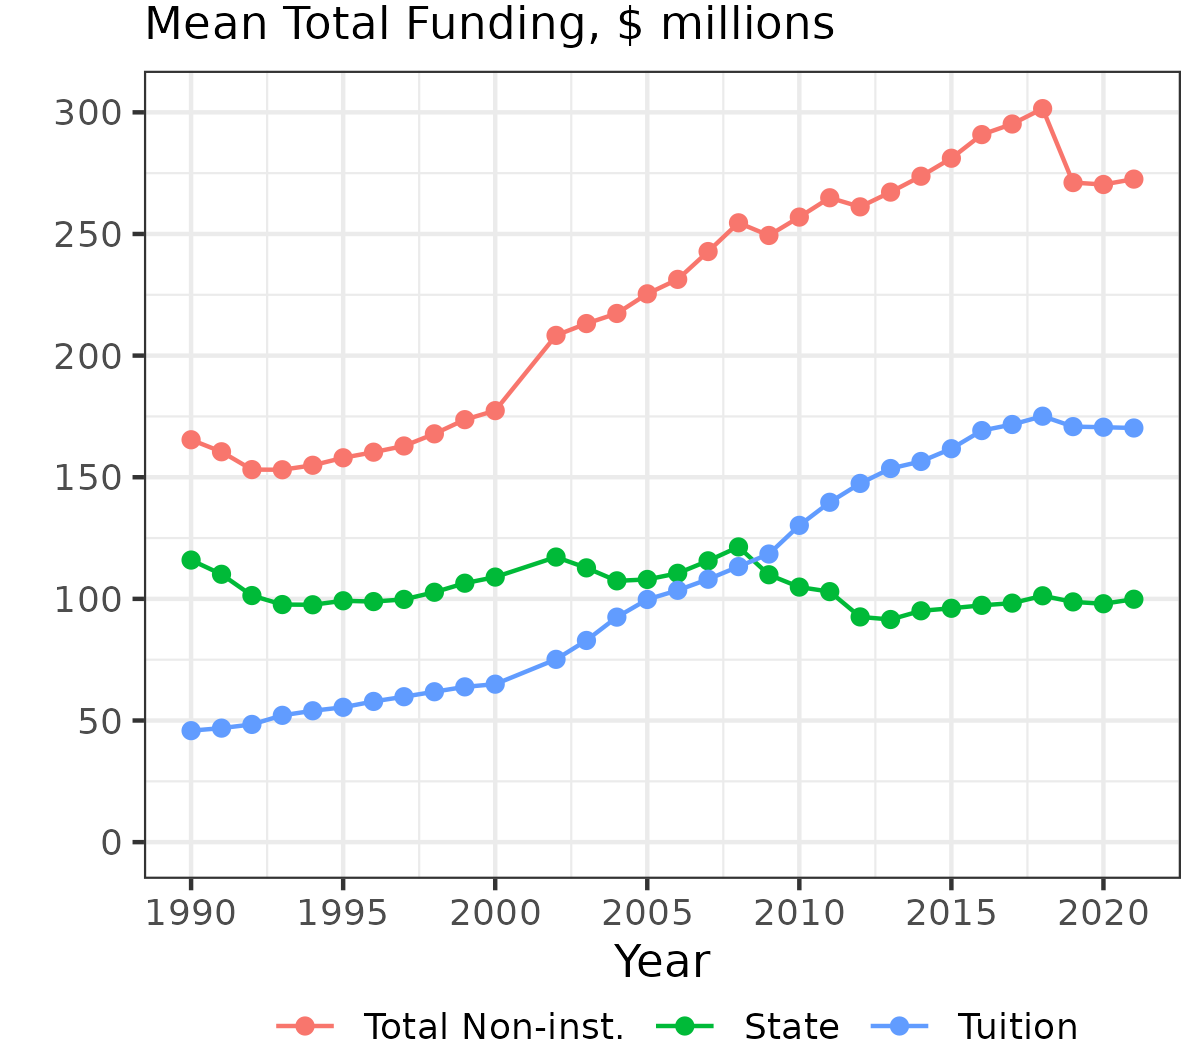
\includegraphics[width=\textwidth]{figures/mean-funding-total.png}
        \label{fig:mean-funding-total}
    \end{subfigure}
    \begin{subfigure}[b]{0.495\textwidth}
        \centering
        \caption{Per Student, \$ 2021 CPI-U.}
        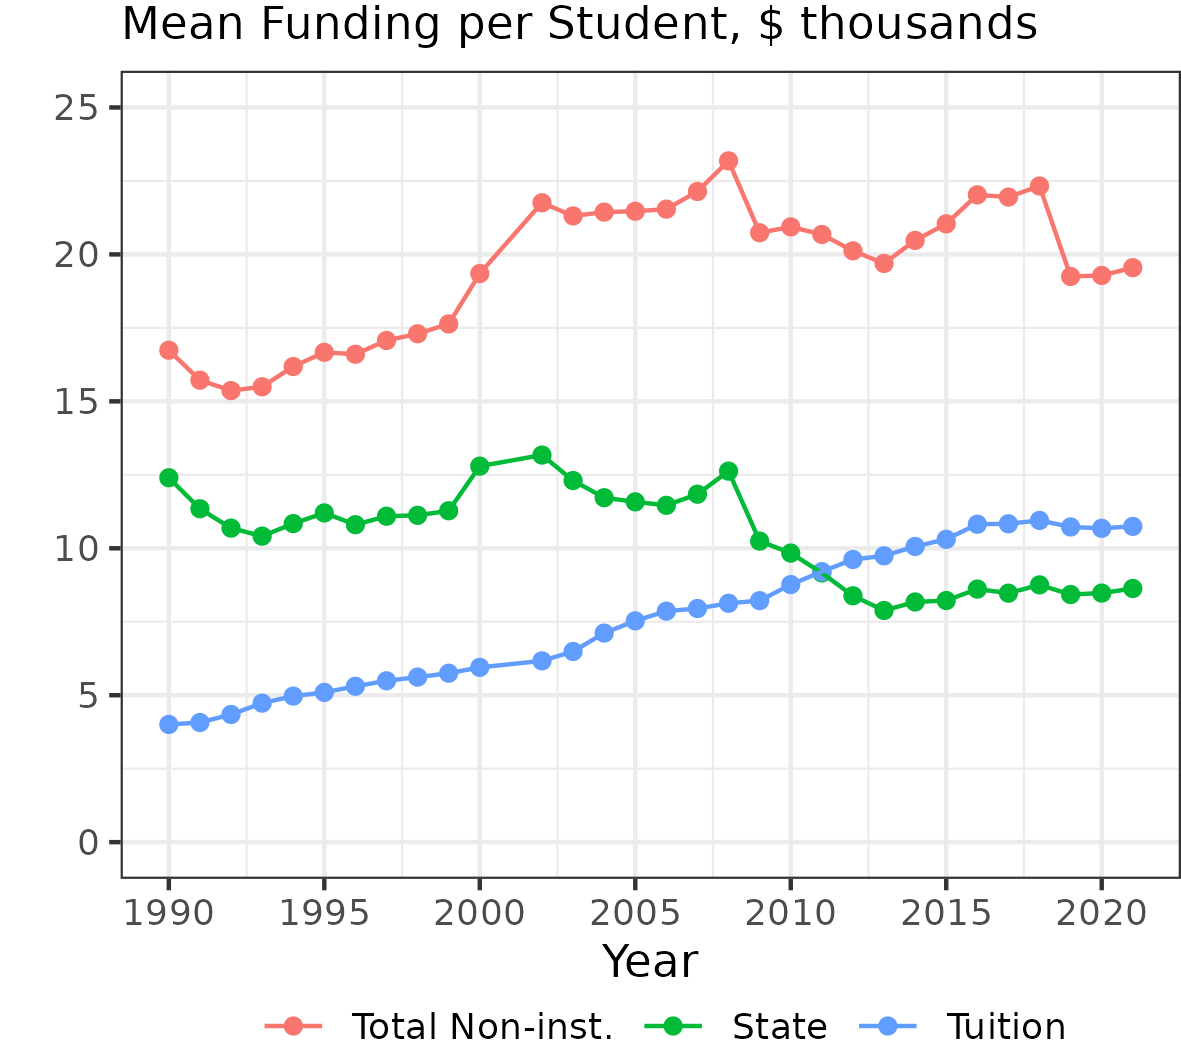
\includegraphics[width=\textwidth]{figures/mean-funding-fte.png}
        \label{fig:mean-funding-fte}
    \end{subfigure}
    \label{fig:funding}
\end{figure}

\begin{figure}[!htbp]
    \centering
    \singlespacing
    \caption{Total Student enrolment, by University Sector and Year.}
    \begin{subfigure}[b]{0.495\textwidth}
        \centering
        \caption{Total Enrolment, Nation-wide.}
        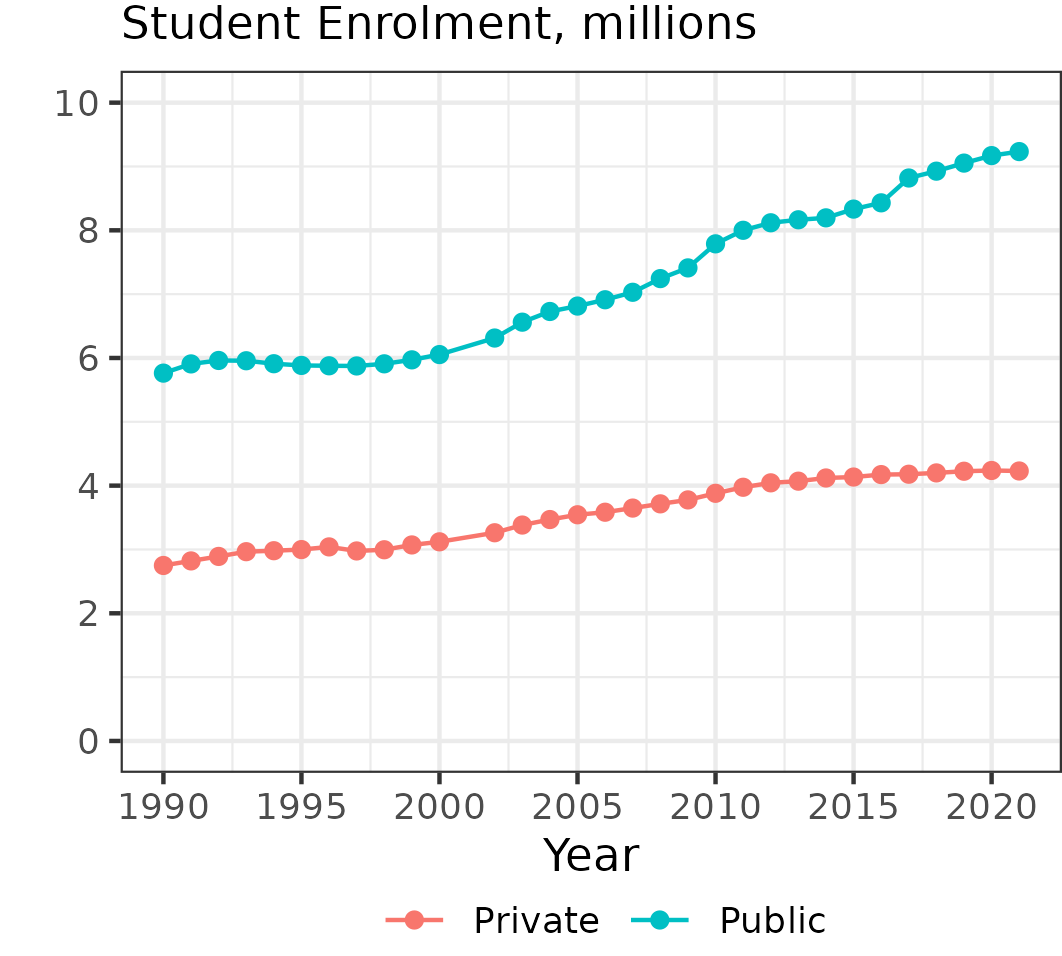
\includegraphics[width=\textwidth]{figures/enrollment-total.png}
        \label{fig:enrollment-total}
    \end{subfigure}
    \begin{subfigure}[b]{0.495\textwidth}
        \centering
        \caption{Mean Enrolment, per University.}
        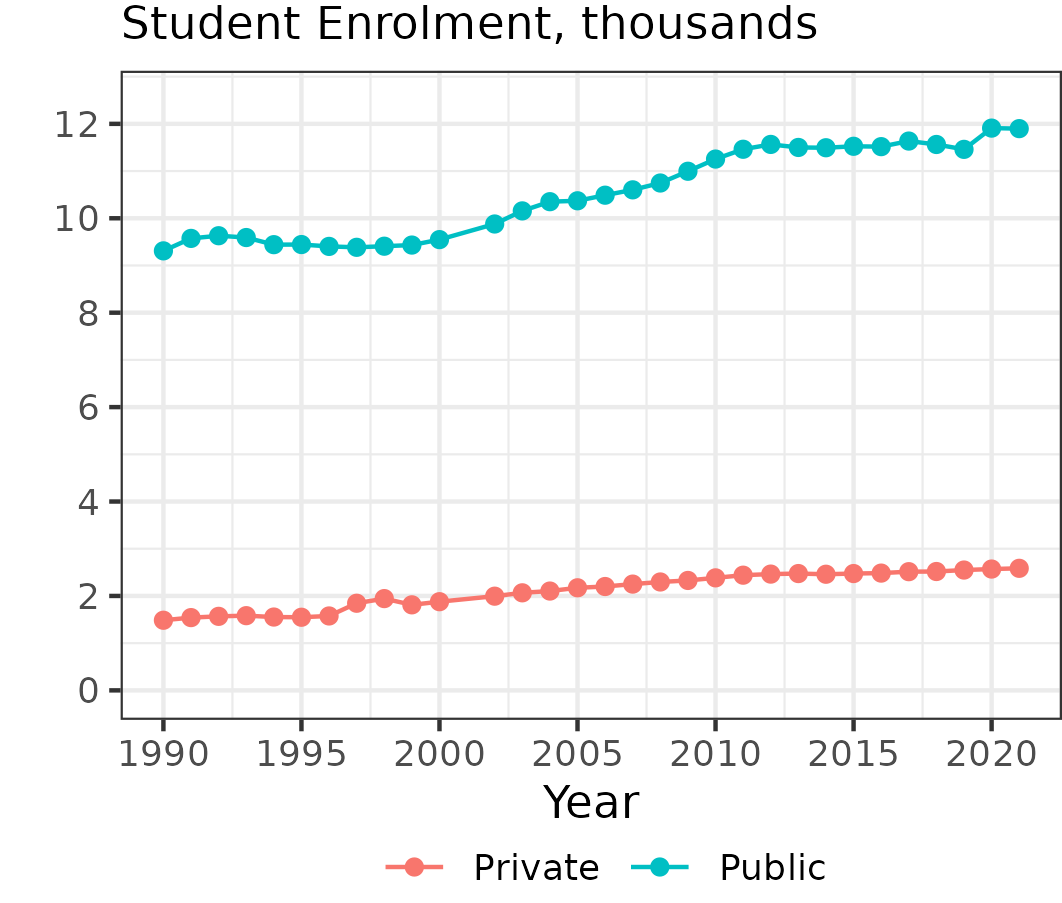
\includegraphics[width=\textwidth]{figures/enrollment-mean.png}
        \label{fig:enrollment-mean}
    \end{subfigure}
    \label{fig:enrolment}
\end{figure}

At the same time, student enrolment at public universities rose precipitously.
6.2 million students were enrolled in public universities in 1990, and this number rose by 47\% to 9.1 million, with most of the increase occurring over the years 2000-2021.
\autoref{fig:enrolment} shows that total enrolment at private universities has also risen over the same time period, but not as drastic in either relative or absolute terms; the mean private university grew from 9,800 students in 1990 to 11,800 in 2021.
This means that revenues per student have stagnated across all measures (seen in \autoref{fig:mean-funding-fte}), and particularly fallen from a mean of \$11,000 per student in 1990 to less than \$8,000 per student in 2021.

\begin{figure}[h!]
    \centering
    \singlespacing
    \caption{Trends in Mean Student Enrolment per Professor, by University Sector and Faculty level.}
    \begin{subfigure}[b]{0.495\textwidth}
        \centering
        \caption{Lecturer.}
        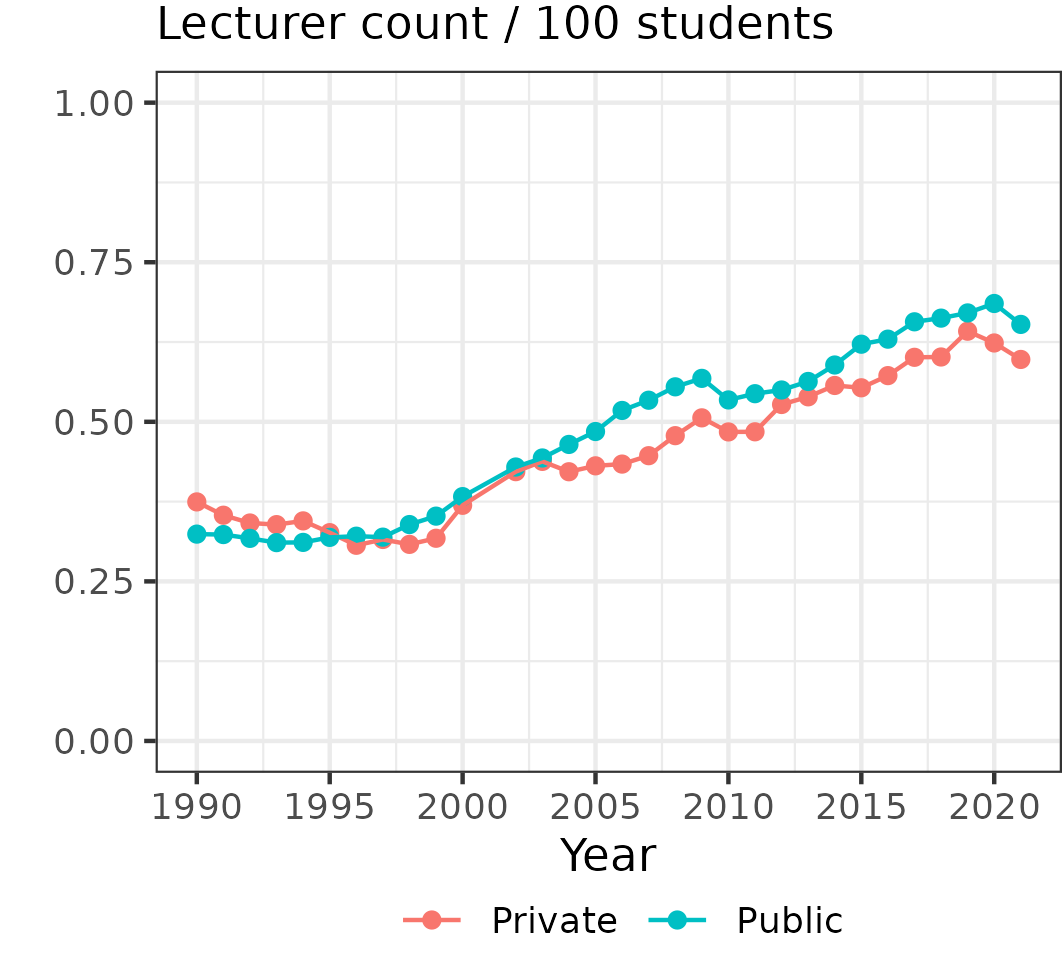
\includegraphics[width=\textwidth]{figures/lecturer-fte-perprof.png}
        \label{fig:lecturer-fte-perprof}
    \end{subfigure}
    \begin{subfigure}[b]{0.495\textwidth}
        \centering
        \caption{Assistant.}
        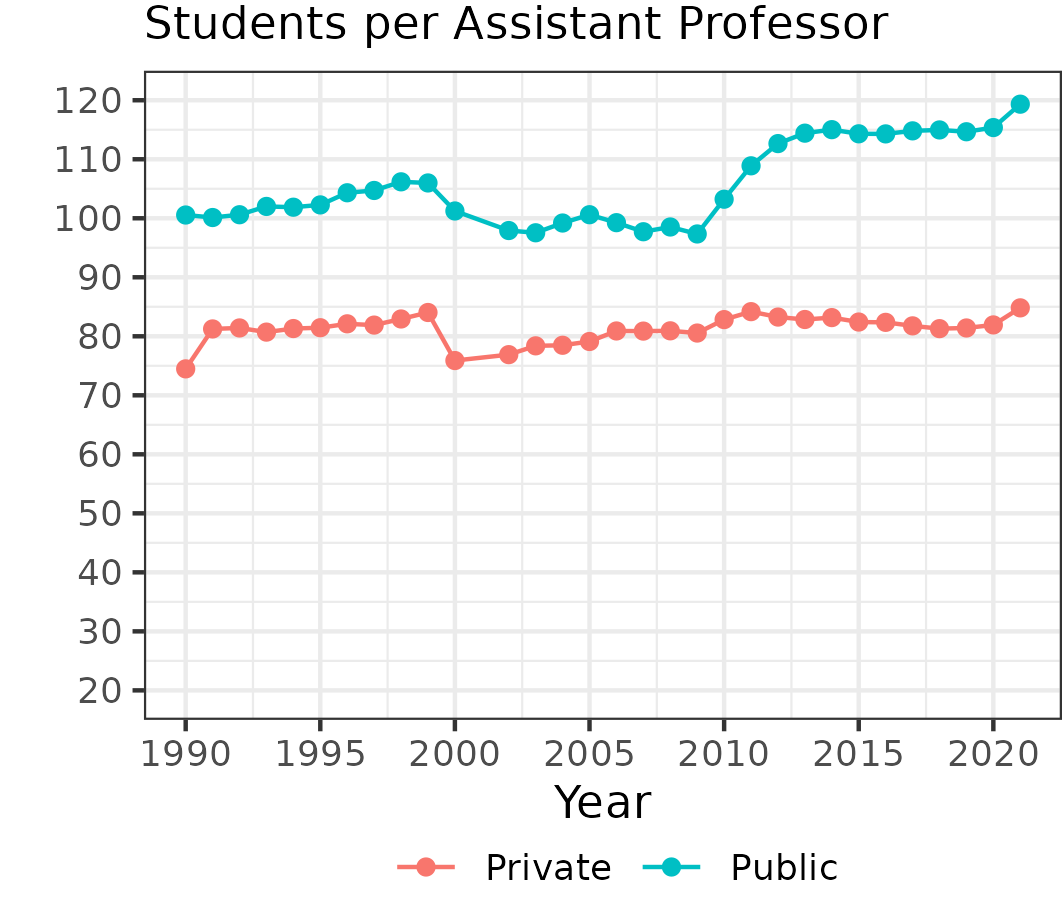
\includegraphics[width=\textwidth]{figures/assistant-fte-perprof.png}
        \label{fig:assistant-fte-perprof}
    \end{subfigure}
    \begin{subfigure}[b]{0.495\textwidth}
        \centering
        \caption{Full.}
        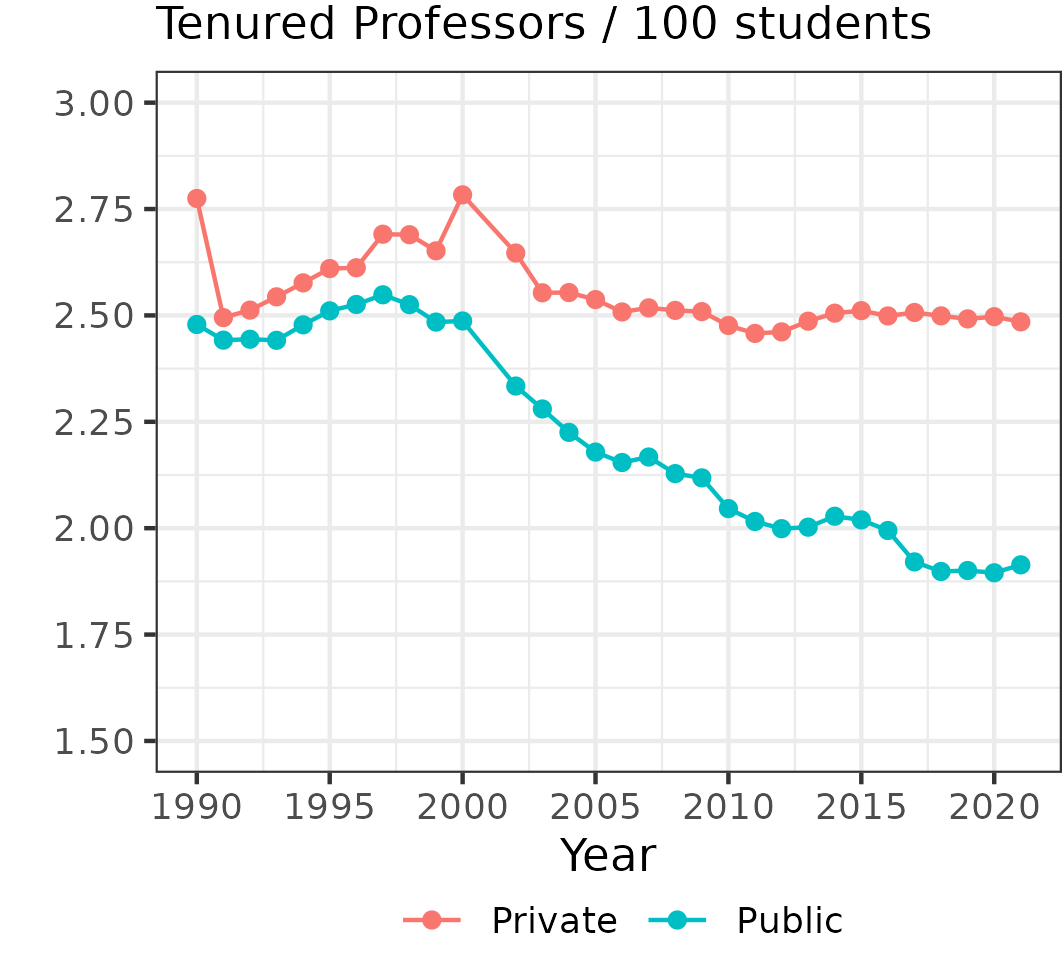
\includegraphics[width=\textwidth]{figures/full-fte-perprof.png}
        \label{fig:full-fte-perprof}
    \end{subfigure}
    \begin{subfigure}[b]{0.495\textwidth}
        \centering
        \caption{All.}
        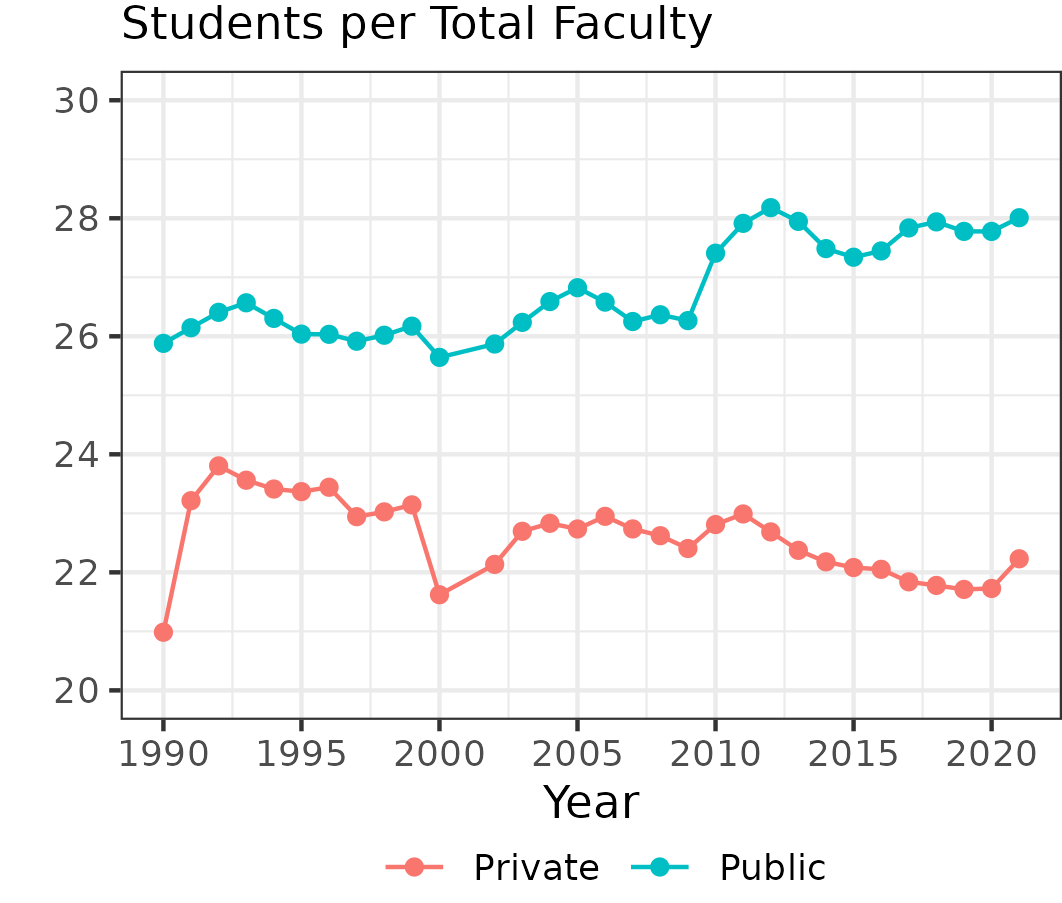
\includegraphics[width=\textwidth]{figures/all-fte-perprof.png}
        \label{fig:all-fte-perprof}
    \end{subfigure}
    \label{fig:fte-perprof}
\end{figure}

There are large differences in the average number of professors per student between the private and public sector.
\autoref{fig:fte-perprof} shows that private universities start with  a higher baseline of around 4.5 professors per 100 students, and exhibited yearly variation of less than 0.5 professor per hundred students over the thirty years.
Public universities start with 3.9 professors per hundred students, and this number falls to around 3., with the largest fall in the 2008-2011 time period.
We see a similar difference in baseline, and fall for the years 2008-2011 for assistant professors.
Private and public universities have similar numbers of associated and full professors before the year 2000, yet this number has fallen by over 20\% in the next 20 years only for public universities: in 2021 the mean public university has 6 fewer full professors per hundred students than the mean private university.
Over the same time period, we see the rise in use of non-tenure track instructor positions (referred to as lecturers from here on), who were employed at similar rates in both sectors in 1990, yet have been utilised by public universities at a higher rate since.

\subsection{Trends in Illinois}
\label{sec:trends-illinois}

The rate that Illinois funds higher education has stagnated to a similar extent as the average for the entire country.
\autoref{fig:illinois-funding} shows the trends for funding sources among the seven Illinois public university campuses, including the falling share of state funding and substitution towards tuition revenue.

\begin{figure}[h!]
    \centering
    \singlespacing
    \caption{Mean Funding Sources among Illinois Public Universities, by Year.}
    \begin{subfigure}[b]{0.495\textwidth}
        \centering
        \caption{Total, \$ 2021 CPI-U.}
        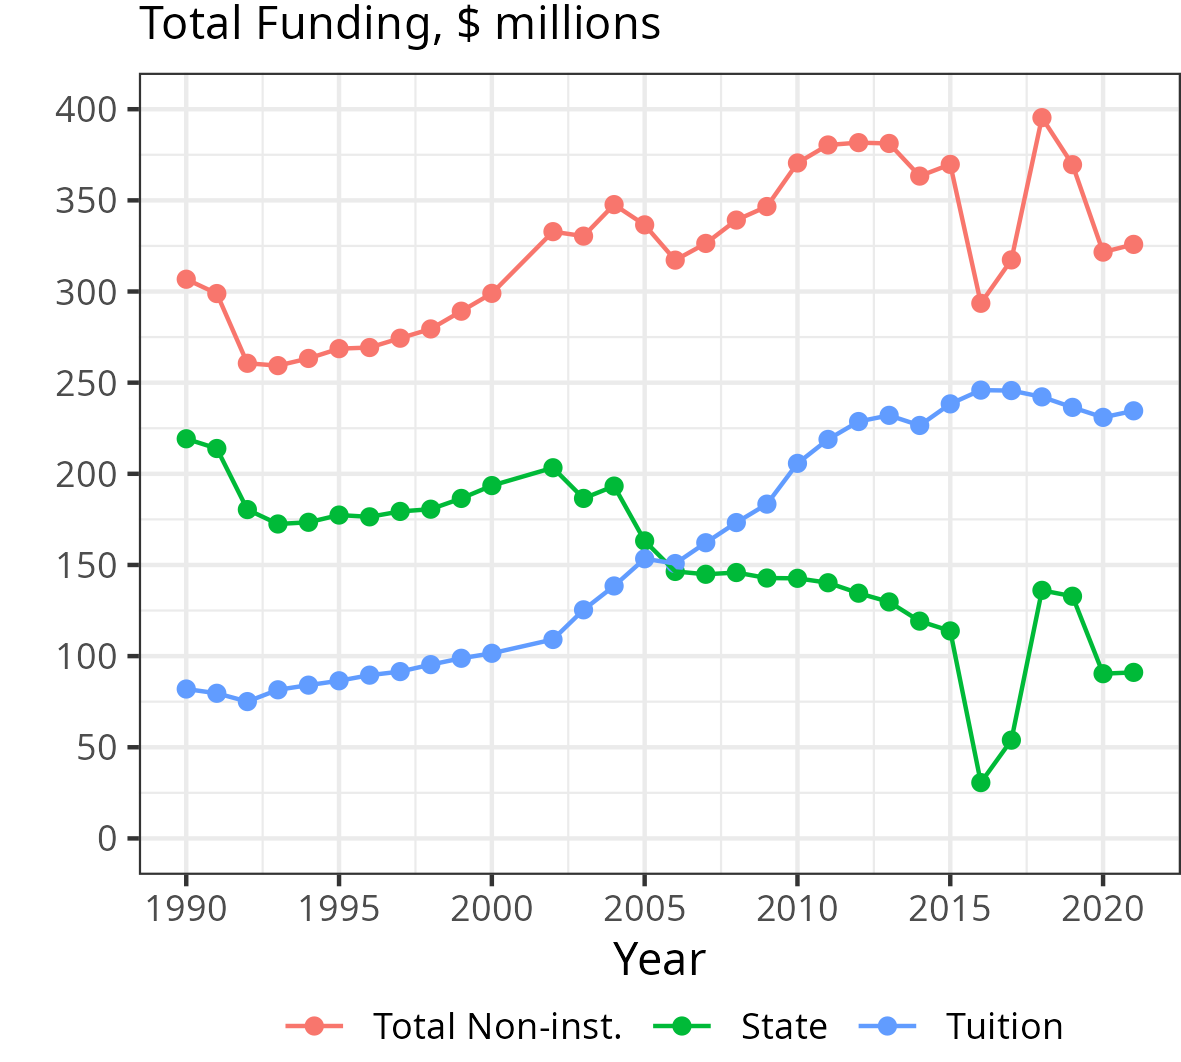
\includegraphics[width=\textwidth]{figures/illinois-funding-total.png}
        \label{fig:illinois-funding-total}
    \end{subfigure}
    \begin{subfigure}[b]{0.495\textwidth}
        \centering
        \caption{Per Student, \$ 2021 CPI-U.}
        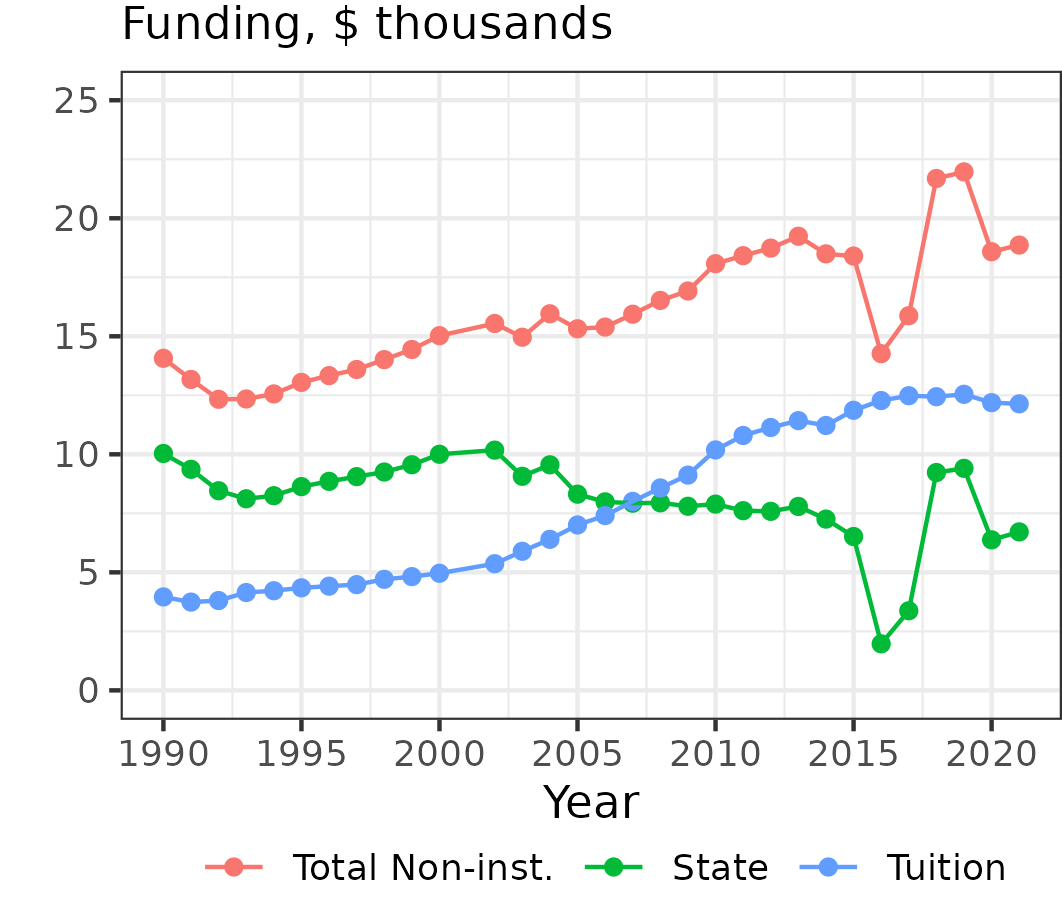
\includegraphics[width=\textwidth]{figures/illinois-funding-fte.png}
        \label{fig:illinois-funding-fte}
    \end{subfigure}
    \label{fig:illinois-funding}
\end{figure}

The decade of 2010--2021 has also seen yearly variation in its revenues, particularly around 2016.
In the calendar year 2015 partisan disagreements between the democratic legislature and republican governor led to the 2016 fiscal year starting with no state budget.
State agencies, and higher education institutions, employed accounting techniques to continue operating without any resources provided by the state government.\footnote{
    Fiscal year 2016 refers to June 205 to June 2016, so is the same as the academic year definition.
}
While public universities were able to stay open, there were drastic revenue and spending cuts in response to the budget impasse, as it continued through fiscal year 2017, and ended with a new budget restoring funding to state institutions for 2018.
This variation in public university revenues via the state funding channel, stemming entirely from political disagreements --- not from state decisions regarding higher education and its finances \citep{young2020squandered} --- mean that Illinois public universities exhibit sizable changes in their state funding over 2010-2021, of similar order to those for the rest of the country over 1990--2021.

% Conceptual Framework
%%%%%%%%%%%%%%%%%%%%%%%%%%%%%%%%%%%%%%%%%
%% Section on possible outcomes
\section{Conceptual Framework}
\label{sec:conceptual}

Universities can respond multiple ways to state funding cuts.
\cite{NBERw23736} established that public universities experiencing state funding cuts did not fully off-set by raising tuition, and instead cut spending.
It is not clear how these funding or spending cuts went on to affect faculty --- or whether they affected faculty at all.

Wider changes in the American higher education sector could concurrently explain the trends in state funding and faculty substitution.
College selectivity changed drastically over the 21st century, where the top universities have become more selective while the average university less selective \citep{hoxby2009changing}.
While the average public university is becoming less selective, it is possible that their most productive or research-focused faculty more often move to more selective and prestigious (and often private) institutions, leaving public universities substituting toward lecturers over time.
This is one way in which the trends may be concurrent, but not causally related.
I address this issue by using shift-share IV approach to isolate funding cuts that affected more funding-intensive universities, measuring the rate of substitution between lecturers and professors in response to yearly changes in state-wide funding.

Universities could respond to funding cuts by cutting faculty salaries, leading to more faculty leaving for jobs at other universities.
Multiple universities passed a university-wide pay-cut for their faculty in response to state budget cuts around the 2008 recession, and Cornell University implemented a professor salary cut in 2020 at the onset of the Covid-19 pandemic.\footnote{
    The Cornell University administration expected large fiscal squeezes in mid-2020, so imposed a faculty salary cut, and then returned the amount cut later in 2020 when the financial squeeze did not materialise.}
Funding cuts could also limit the salaries public universities can offer to new faculty hires, leading to fewer or less accomplished faculty accepting offers at public universities.\footnote{
    Faculty often consider their outside options in job decisions, considering offers for employment and/or promotion from multiple universities at the same time --- see \cite{blackaby2005} for an overview of faculty outside options.
    If public universities can only make low salary offers thanks to funding cuts, then they are less likely to land professors with multiple offers.
}
This effect may not be the same across faculty seniority; most universities hire more junior faculty each year, so that yearly hiring disruptions may disrupt the looser market for established full professors more than tighter market for assistant professors or lecturers.
While these factors make it unclear who will be affected most by funding cuts, there is one empirical fact worth noting: lecturers have substantially lower annual salaries than professors.
The average Illinois assistant professor's annual salary is $\$76,897$, tenured professors' is $\$109,283$, while lecturers' is $\$31,449$ (annual salary for 2010--2021 in 2021 USD, see \autoref{tab:illinois-summary}).
If a public university's primary obligation is to teach, and they must fulfil this objective with less funding, then substituting away from tenure-track and tenured professors towards lecturers is rationalisable purely on this basis.

If faculty are affected by state funding cuts, then it is still not clear whether effects are persistent or merely transitory.
Universities employ professors on multiple-year contracts (e.g., the tenure contract), and decisions to retire, move university, or leave academia are multiple-year commitments, so that it may take multiple years for effects to trickle down to faculty.
On the other hand, university departments hire in annual cycles, so that a funding cut in one year may immediately impact faculty hiring in the same year, and thus faculty counts in the next academic year.
% Yet, it could be the case that faculty hiring resumes the very next year, or even hires more to compensate for last year's cancelled hiring cycle.
%This means that state funding cuts could effect faculty in only transitory changes in faculty counts.
As such, this paper investigates the dynamics of state funding cuts and their effects on faculty, by employing local projections methods to measure the persistence of effects for multiple years following a state funding cut.

% Empirical methods
%%%%%%%%%%%%%%%%%%%%%%%%%%%%%%%%%%%%%%%%%
%% Empirical section
\section{Empirical Framework}
\label{sec:empirics}

This paper identifies the effects of changes in state funding on faculty.
However, a university's state funding is not exogenous to state decisions for support of higher education, or exogenous to internal institutional decisions.
Instead, the state government and university administration undertake a complex process of allotting resources across multiple different priorities, including instruction, research, or between departments.
For example, it may be the case that a state government restricts funding for only its lowest performing universities in response to a budget shock, introducing a treatment selection-on-outcome threat to identification. 
Importantly, funding from a university's state government provides opportunity to address such endogeneity.

\subsection{State Funding Shocks}
\label{sec:approp-shocks}

I use a shift-share instrument to address endogeneity concerns for the amount of funding a state allots to each of its public universities.
\cite{NBERw23736,NBERw27885} develop the instrument for public university finances by exploiting a shift-share instrument for changes in state-level funding interacted with university reliance on state funding in a base period.
\begin{align}
    \label{eqn:public-instrument}
    Z_{i,t} &\coloneqq - \left[
    \left( \frac{\text{Total State Funding}_{s(i),t}}{\text{Student Population}_{s(i),t}} \right)
    \sum_{\tau = 0}^{3} \frac 14
    \left( \frac{\text{State Funding}_{i,1990 + \tau}}{\text{Total Revenues}_{i,1990 + \tau}} \right) \right]
\end{align}
The system exploits the fact that institutions who rely on state funding more will be affected by state funding shocks.
$Z_{i,t}$ is the instrument for state funding for institution $i$ in year $t$, interacting the average funding for universities in state $s(i)$ with reliance on state funding relative to total revenues, averaged across the base years 1990--1993.\footnote{
    1990--1993 are defined as data for public university finance data are most comparable (i.e. without many missing values) beginning in 1990.
    \cite{NBERw23736} use the single year 1990 as the base year, though I use the four years to ameliorate missing values in the single year of 1990.
    Results are similar in either specification.
}
$Z_{i,t}$ is constructed as negative to reflect the fact that the long term trend in, and most of the short-run shocks to, state funding for higher education have been negative.\footnote{
    When used in log terms, the instrument is the negative of the logged shock --- i.e., $- \log \left( -Z_{i,t} \right)$ as opposed to log of the negative shock $\log Z_{i,t}$ directly.
}
State funding has been falling, so that the instrument describes shocks to university revenues, mostly in a negative direction.\footnote{
    \label{foot:control}
    \cite{NBERw27885} note the tendency for public universities to respond to state funding cuts by increasing reliance on tuition, where \cite{NBERw23736} specifically instruments for tuition revenues with collected information on legislative tuition price controls.
    It may be argued that tuition revenues are confounder between the causal effect of changes in state funding on a university's total revenues, so that this analysis focuses on state support for higher education (not total revenue), as do \cite{NBERw27885}.
    On the other hand, rises in tuition revenues (per student) may arise as result of tuition hikes thanks declining state support, which would mean controlling for tuition would constitute a bad control.
    Nonetheless, estimates including tuition revenues (per student) as a control in the second stage of the IV estimates produces results of very similar magnitude and direction, and so are omitted.
}
The instrument approach relies on the conditional independence assumption, that the instrument is independently assigned to the universities.
While this assumption is fundamentally untestable, we see that universities are by-in-large smaller (in terms of enrolment, total revenues, and professor count) at the top of the state funding shock distribution (see~\autoref{tab:summary-quantiles}).
Though on a per student basis, there is little difference across the distribution (except in the outcomes under consideration).
The state funding shock instrument is positively associated with the total enrolment and total amount of state funding for each university, in both \$ and $\log$/percentage change terms, while other the other sources of university finances are not associated with the funding shock.
So that the other sources of finances are not clear confounders for the instrumental variables strategy, as they exhibit balance with respect to the funding shock instrument \citep{pei2019poorly}.
Yearly and individual fixed effects are included in regressions throughout to implicitly condition on mean differences between universities and years, leading to the assumption of conditional independence of the instrument with respect to state funding for each public university.

The state funding shock is an instrument the level of state funding for each university in each year.  
The first-stage is then as follows, including institution and year fixed effects, where $X_{i,t}$ represents the amount of state funding divided by the number of full-time students attending the university.
\begin{equation}
    \label{eqn:firststage}
    X_{i,t} = \eta_i + \zeta_t + \delta Z_{i,t} + \epsilon_{i,t}
\end{equation}
We note the conditions for exogeneity in the instrument (following the discussion presented by \citealt{NBERw27885}).
The instrument is exogenous if state policy decisions for funding of public universities are uncorrelated with unobserved institutional changes of any specific college or university in the state \citep{borusyak2022quasi}.
This assumption is plausible given that the majority of states have multiple (i.e., more than five) public universities, without any single university campus receiving the majority of state funding within any single state.
Secondly, the shift-share identification strategy requires exogeneity in either the base-line share or shift component of the instrument.
In this case, we satisfy the second: universities' institutional-level decisions are not correlated with contemporaneous or upcoming shocks to state funding.\footnote{
    It would be plausible to consider the case that universities make institutional-level decisions in a consistently different manner to those 
    with differing reliance on state funding in 1990, so that exogeneity by the base-line share is not plausible here.
}
Lastly, the shift-share approach assumes that state funding shocks affect faculty outcomes only via affecting university finances.

The shift-share instrument has a strong first stage for universities' yearly state funding.
\autoref{tab:firststage-reg} presents results of the first-stage regression, separately with and without a control for tuition revenue per student, plus institution and year fixed effects.
\autoref{tab:firststage-reg} Panel A shows estimates of a funding shock of \$1 per student in the state on state funding per student at the university, and Panel B the \% increase effects of a 1\% increase in the shock per student on state funding per student.
Column (1) shows that a funding shock of \$10 (per student in the entire state) is associated with \$11.76 less state funding per student at the university, with the corresponding -10\% funding shock leads to -9.77\%
less funding (column 1, panel B), with similar estimates with and without including fixed effects.
Column (2) shows estimates of the first-stage without including fixed effects, and gives less precise estimates for the funding shock, likely thanks to systematic differences in universities unaccounted for without fixed effects.
Columns (3) and (4) include the tuition revenue control (explained in \autoref{foot:control}) to exhibit estimates with the inclusion of this possible collider (or bad control).
Column (3) shows similar estimates to column (1) in both Panels A and B thanks to inclusion of fixed effects, so that the uncertainty in including tuition revenue as a possible bad control for the level of state funding does not matter thanks to the inclusion of fixed effects.
Column (1) represents the estimates for \autoref{eqn:firststage} with fixed effects, omitting the tuition revenue control, and is the preferred form that I proceed with.

These results, together with the case for exogeneity, show the funding shock instrument strongly predicts university revenues in the first-stage estimation.


\subsection{Instrumental Variables Model}
\label{sec:iv-model-uni}

I use the instrument defined in \autoref{eqn:public-instrument} to overcome the endogeneity concerns for state funding to each public university, so the primary empirical model is an instrumental variables model.
\autoref{eqn:firststage} is the first stage for exogenous variation in the state funding for university $i$ in year $t$, and \autoref{eqn:secondstage} the second stage for the effect of state funding on faculty outcomes.\footnote{
    It is important to note the treatment effect isolated here; the instrumental variables approach identifies the local average treatment effect, one weighted to level of exposure when treatment is continuous as is the case here.
    So we interpret this treatment effect as a weighted average of effects on faculty at public universities to state funding changes, specific to state funding shocks, among the complier group --- i.e., among universities who respond to funding shocks and would not have made faculty-outcome changes absent the funding shock.
    Also, we assume that no universities state funding increased in response to the negative state funding shock (monotonicity).
}
\begin{equation}
    \label{eqn:secondstage}
    Y_{i,t} = \alpha_i + \gamma_t + \beta \widehat X_{i,t} + \varepsilon_{i,t}
\end{equation}
I estimate the system by two stage least squares, including institution and year fixed effects.\footnote{
    Note that dividing by student count also implicitly controls for the size of the university, so that this model implicitly accounts for yearly variation in professor count and university revenues arising from a university's size of growth/decline.
}
$Y_{i,t}$ represents faculty outcomes for university $i$ in year $t$, $\alpha_i, \gamma_t$ university and year fixed effects, and $\widehat X_{i,t}$ state funding for university $i$ estimated in first stage \eqref{eqn:firststage}.

Additionally, I investigate the effect of changes in state funding among incumbent professors.
Incumbent professors are faculty who are already employed at the university; state funding changes may affect faculty who are already at the university (beyond affecting whether they get hired), so I base the instrument in the year that the professor was hired, and include fixed effects for the hiring year.\footnote{
    This formulation follows that presented by \cite{NBERw27885}, where individual student outcomes are analysed via variation in state funding after their freshman-year.
    This contrasts with \autoref{sec:iv-model-uni} and \cite{NBERw23736}, where the unit of analysis is the university-year, where base year 1990 is more appropriate.
    See \autoref{sec:iv-model-indiv} for the instrument and second-stage specification.
}
The instrument exogeneity and exclusion follows the same argument as above, where the Illinois legislature did not target any single campus for funding cuts and no single Illinois campus takes the majority of state funding.

It is not a priori clear which units are appropriate for this analysis;
does it make sense to consider state funding in purely dollar amounts per student, or in percent change rate?
The funding shock instrument is a strong predictor for the average university's level of state funding in either unit; a funding shock of \$1,000 per student in the entire state leads to around \$1,176 per student at the university, while a funding shock of $-10$\% leads to around 9.77\% less state funding per year.
Yet, the level of state funding (and the outcome variables) vary greatly between states for the unit of analysis.
For example, the average Illinois public university receives \$10,709 in state funding per student in 1990 and  \$6,713 in 2021 (a fall of over 30\%), while California went from \$19,224 per student to \$12,915 in the same time span (a fall of 37\%).
While most states are not exactly the same to California and Illinois, this is example is telling for the phenomenon of stagnating state funding:
states vary in their absolute funding for higher education in 1990, but most have experienced a decline of similar order to 30\%, so that the stagnation in state funding has been a percent change trend over this time period.
As such, I include regression specifications where the explanatory and outcome variables are $\log$ transformed, and refer to these when stating results in percent change terms.

\subsection{Effects in Years After the Initial Funding Shock}
\label{sec:local-projections}
The effects of a change in the universities funding may not be immediate, and faculty may be affected multiple years after a funding shock.
Yet, the funding shock instrument is significantly auto-correlated year-on-year; a large state-level funding shock in year $t$ is also likely to experience a large funding shock in year $t-1$.
Similarly, funding shocks to higher education in a year are highly correlated with state funding per student in the 5 years before and after the initial shock in IPEDS data (see \autoref{fig:lag-firststage}).
Thus, a linear model correlated state funding in year $t$ with outcomes in year $t+k$ will suffer from time-series confounding.

I employ a local projections approach to model how faculty outcomes in years $t+k$ are affected by state funding in year $t$, for future years $k > 0$ \citep{jorda2005}.
The local projections method is an empirical model used to estimate dynamic treatment effects when the treatment is not binary, so that time-series confounding (i.e., treatment in time $t$ is correlated with treatment in time $t-1$) is present \citep{montiel2021local}.
This method estimates the effect of treatment $X_{i,t}$ on outcome $Y_{i, t+ k}$ in follow-on years $k > 0$, while accounting for the auto-correlation between the other years.\footnote{
    The funding shock has a persistent effect on state funding, multiple years after the initial funding shock, so that the instrument is similarly strong for the local projections method (see \autoref{fig:firststage-lp}).
}
Additionally, the approach accomodates use of an instrument for state funding \citep{olea2021inference}, so that I use the shift-share instument in local projections estimates as in the rest of the empirical analysis.
I present estimates in graphical form, where the $x$-axis represents the year relative to the funding shock (i.e., $x = 0$ represents the year of the state funding shock) and the $y$-axis represents the estimated effect of the funding shock on that year's outcome.\footnote{
    See \autoref{fig:count-lp} for the graphical format, and the corresponding note for further explanation.
}

% Empirical results
%%%%%%%%%%%%%%%%%%%%%%%%%%%%%%%%%%%%%%%%%
%% Results section
\section{Results}
\label{sec:results}

\subsection{First-Stage Estimates}
\label{sec:results-firststage}
The shift-share instrument has a strong first-stage for universities' yearly state funding.
\autoref{tab:firststage-reg} show results of the first-stage regression among IPEDS data, separately with and without a control for tuition revenue per student.
\autoref{tab:firststage-reg} Panel A shows estimates of a state funding shift-share of \$1 per student on state funding per student at the university, and Panel B the effects of a 1\% increase in the state funding shift-share on state funding per student.
Column (1) shows that a state funding shift-share of \$10 per student is associated with \$11.76 less state funding per student at the university; $-10$\% state funding shift-share leads to $-9.77$\% state funding per student at the average university.
Estimates are presented for specifications with and without fixed effects.
Column (2) shows estimates of the first-stage without including fixed effects, and gives less precise estimates for the funding shift-share --- this may be due to systematic differences in universities, which are not accounted for when omitting fixed effects.
Columns (3) and (4) include the tuition revenue as a control (explained in \autoref{foot:control}) to exhibit estimates with or without this control variable.
Column (3) shows similar estimates to column (1) in both Panels A and B thanks to inclusion of fixed effects, so whether tuition revenue is a bad control does not affect empirical estimates.
Column (1) represents the estimates for \autoref{eqn:firststage} with fixed effects (not including tuition revenue as a control variable), and is the preferred specification that I proceed with;
all specifications (except column 4 in both panels) have a large F statistic on the excluded instrument.\footnote{
    I calculate the F statistic on the excluded instrument, while also accounting for fixed effects and two-way standard error clustering, by the methods provided in \cite{olea2013robust}.
}
I use the same empirical strategy in the analysis of Illinois faculty, and \autoref{tab:firststage-illinois} presents first-stage estimates among the IBHED data; results are similar to those calculated in IPEDS data.
These results show the funding shift-share instrument strongly predicts a university's state funding in the first-stage estimation.

The first-stage is strong in both IPEDS and IBHED data, and the argument for exogeneity comes from independence of the state funding mechanism to any individual public university campus (as in \autoref{sec:empirics}).
The IV approach also assumes that shifts in state-wide funding for higher education (the instrument) affect outcomes only via affecting state funding for the university (exclusion restriction).
This assumption is fundamentally untestable, but is bolstered by the lack of relationship with university characteristics.
\autoref{tab:summary-quantiles} shows the mean of various university variables, across the instrument distribution.\footnote{
    The shift-share instrument is correlated with tuition revenues (and thus the sum of non-institutional revenues), so could be a presenting a threat to endogeneity.
    As mentioned above, including tuition revenue as a control (even though it could also be a bad control) does not meaningfully change first- and second-stage results in any specification, rendering this plausible threat to identification moot.
    See \autoref{foot:control} and \autoref{tab:firststage-reg}.
}
The university--years in the bottom 20\% of the instrument distribution have more research spending than those in the next 20\%; this is to be expected, as university spending is heavily related to state--wide shifts in funding.
On the other hand, the measures of selectivity (acceptance rate, 6--year graduation rate) are noticeably different across the distribution of the instrument.
While the shift--share instrument exhibits balance for many relevant university characteristics (except tuition revenues and selectivity), I include institution and year fixed effects throughout my analysis, effectively controlling for any possible confounding effects of differences between universities.

Do state funding cuts meaningfully affect universities?
While the shift-share performs well in predicting state funding (i.e., a strong instrument), it could be the case that the day-to-day operations of a university are not affected.
University could have responded to state funding cuts by cutting areas of spending unrelated to research or instruction, or fully off-set the cuts by charging higher tuition fees, leading to no effects on the university or faculty.
To allay this concern, I estimate the IV model on IPEDS data for areas of university spending  (\autoref{tab:expenditures-shock-reg}).
This exercise gauges the effects of state funding cuts on areas of university spending to gauge whether the first-stage is economically meaningful, and to see which areas of higher education operations are affected by state funding cuts.
Following a state funding cut, universities spend less on instruction, student services, operations, and grant aid.
Additionally, they charge higher tuition fees, though this rise is at most a quarter of the state funding cut, so does not come close to fully off-setting state funding cuts.
These results are in line with previous work showing state funding cuts (or tuition price limits) reduce student-focused spending \citep{NBERw23736}, financial aid \citep{miller2022making}, and lead to increased tuition fees \citep{bound2019public,webber2017state}.

\subsection{University Level, IPEDS}
\label{sec:results-ipeds}
State funding cuts lead to measurable changes in the number of faculty at US public universities.
\autoref{tab:facultycount-shock-reg} presents OLS and IV estimates for the effect of state funding cuts on the number of faculty at public universities, separately for each faculty position (lecturer, assistant and full professors, total).
The results are presented in two different units: Panel A shows how a \$1 increase in state funding changed the count of faculty per students, while Panel B shows how a 1\% increase in state funding led to a percent change in the number of faculty per students.

An extra \$1,000 in state funding per student leads to the average university employing 6 fewer lecturers, while effects for the other positions are not discernible from zero (\autoref{tab:facultycount-shock-reg}, Panel A).
A 10\% state funding cut lead to a 4.4\% increase in the number of lecturers per student, and a decrease of 1.35\% and 1.37\% for assistant and full professors, respectively.
A state funding cut of 10\% leads to a 0.65\% decrease in the total number of faculty per student (\autoref{tab:facultycount-shock-reg}, Panel B).
These are large substitution effects, and explain roughly 40\% of the trend in substitution towards lecturers over the same time period.
The average public university has roughly 36\% less state funding per student in 2021 than they did in 1990, while employing over double the number of lecturers and 20\% fewer professors (relative to enrolment, seen in \autoref{fig:mean-funding-fte}, \ref{fig:fte-perprof}).

Universities do not re-adjust by hiring more professors to make up for last year's funding cut, and so the substitution towards lecturers becomes persistent.
\autoref{fig:count-lp} shows LP estimates, showing the elasticity for professor count per student in year $t+k$ with respect to state funding in year $t$ (and cumulative intermediate cuts).
State funding cuts affect the number of lecturers and professors at universities up to 9 years after the initial funding cut.
A 10\% state funding cut leads to 4.2\% (2.9--5.5 in a 95 percent confidence interval) more lecturers per student the following year, and around 3.1\% (0.6--5.5 confidence interval) more lecturers nine years later.
A 10\% state funding cut leads to 1.5\% (0.6--2.2 in a 95 percent confidence interval) fewer assistant professors per student the following year, and around 1.1\% (0.2--2.0 confidence interval) fewer nine years later;
the same cut leads to 1.2\% (0.6--1.8 in a 95 percent confidence interval) fewer full professors per student the following year, and around 0.9\% (0.1--1.7 confidence interval) fewer nine years later.

These effects are a substitution of professors for lecturers at public universities, as the total number of faculty per students are relatively unrelated to funding cuts, but the lecturer count increases and professor count decreases.
This agrees with a model for universities departments having fixed teaching requirements making human-resources decisions under constrained resources (e.g., \citealt{abe2015implications}), lending credibility to this type of model for understanding recent human resources decisions of public universities.
Furthermore, if a university must teach more students, but cannot afford to hire a full-time professor who teaches 2--3 classes a year, then it makes sense that they hire 2--3 additional lecturers on part-time contracts for each class as a replacement.
This provides simple intuition for why the lecturers' elasticity is 2--3 times larger than that for assistant/full professors in \autoref{tab:facultycount-shock-reg}.
While no previous research causally connects funding cuts to substituting professors for lecturers, the phenomenon has been alluded to in popular media \citep{wiu2016} and university rankings (where more lecturers hurts a university's ranking, \citealt{usnews2023}).
The results provided here give the first real evidence for such popular claims.

\subsection{Illinois Faculty, IBHED}
Incumbent professors at Illinois universities are relatively unaffected by state funding cuts at their university.
\autoref{tab:faculty-shock-illinois-rolling} show estimates of a 10\% change in state funding per student on faculty salaries, rate of exiting the Illinois public university system, and rate of promotion.
The estimates are not discernible from zero in any specification, including the shift-share IV estimates, so that faculty seem to have little or no state funding cuts passed on to them for these outcomes.

It could be the case that effects on faculty do not materialise until multiple years after a funding cut, though the data do not support this possibility.
LP estimates show that professors' salaries, including salaries, are not significantly affected in years following funding cuts (\autoref{fig:salaries-illinois-lp-rolling}) --- they do not receive lower rates of pay raises, or delayed salary cuts, in response to state funding cuts.
Similarly, promotion rate and rate of exit from the Illinois public university system are also unaffected in later years (\autoref{fig:promoted-illinois-lp-rolling}, \ref{fig:exit-illinois-lp-rolling}).
Lecturers receive a 0.75\% increase in salary in the second and third year after a 10\% increase in state funding (\autoref{fig:salaries-lecturer-illinois-lp-rolling}), though they are they only faculty who saw any effect of state funding cuts in terms of salaries.

These results show that faculty --- both lecturers and professors --- are relatively unaffected by state funding cuts, in the Illinois public university system.
Illinois is a state with a large public university system, relative to student enrolment, with trends in state funding for education similar to national trends, and with both selective and non-selective universities.
If faculty are unaffected in Illinois, then it is unlikely that faculty in the rest of the nation are affected on average.
Note, however, that this analysis studies faculty who are already faculty.
The IBHED data do not measure the entire pool of academics applying for faculty jobs at Illinois universities, but only those who applied to, were accepted, and then started a job as a lecturer or professor.
These are incumbent faculty, and the data show they are unaffected by state funding cuts.
This raises a question: how can funding cuts lead to a large substitution of professors for lecturers, when incumbent faculty are not affected?

\subsection{Impacts on Faculty Hiring}
Turn-over is the primary channel that changes in faculty composition happen, where faculty exit their jobs and new faculty are hired to replace those leaving --- or no more are hired to replace those who left.
\autoref{fig:exit-illinois-lp-rolling} shows that Illinois faculty are no more likely to exit the Illinois system (either retire or take a new job elsewhere) following state funding cuts, so there is one remaining channel for the substitution of professors for lecturers: increased hiring of lecturers and reduced hiring of new professors.

To investigate reduced hiring of new professors, I first investigate faculty hiring rates among Illinois universities from the IBHED data.
To do so, I count the number of faculty new in the panel of all Illinois public university faculty for years 2011--2021, where the panel first year is 2010.
I then use this as the outcome in OLS and shift-share IV regressions, where each observation is an Illinois university--year and data for state funding come from IPEDS.\footnote{
    This is the same specification as the IPEDS analysis restricted to Illinois universities.
    The IPEDS data have yearly faculty counts, but not discern between faculty promotions, quits, and hires; the Illinois data can do so thanks to the panel structure of the data.
}
To study whether these effects hold true nation-wide, I use public on the number of professors at all US public universities for the entire decade 2011--2021, provided by \citep{wapman2022quantifying},
and perform the same analysis to see if state funding affected the number of professors hired.
See \autoref{sec:appendix-hiring} for further details on this data source.

\autoref{tab:facultyhires-illinois-reg} shows these estimates for Illinois public universities.
In general, faculty counts are relatively unrelated to state funding among Illinois universities; though the point estimates line up with analysis in IPEDS, the smaller number of observations mean that the precision of estimates are small and indistinguishable from zero, in both raw counts and in log units.
In the national-level \cite{wapman2022quantifying} data, universities with more state funding hire more professors across 2011--2021.
An extra 10\% in state funding is associated with 8.5\% more professors hired per students, as seen in \autoref{fig:hiring-correlation}.
I use these data as part of a shift-share analysis, showing that a 10\% state funding cut per student leads to 13\% fewer professor hires (relative to enrolment), and that these hires are roughly equal for gender of professor hired.

State funding cuts lead to lower professor hiring, and the persistent funding cuts to public universities led to lower professor hiring across the last three decades.
The channels for faculty turn-over were unaffected by state funding cuts in the analysis of Illinois faculty, while professor hiring is related to funding cuts in both correlational terms and in a shift-share analysis.
Combining these pieces of evidence means that reduced professor hiring was likely the main mechanism for how state funding cuts led to a substitution of professors for lecturers at public universities.

\subsection{Robustness Checks and Heterogeneity Analysis}
\label{sec:results-robustness}
It is possible that the identification strategy is not robust to some confounding issues or trends.
For example, selective institutions may have received funding cuts for other reasons, or states with lower performing institutions or declining populations strategically cut funding for only less selective universities.
I investigate these issues with two different analyses, and then investigate heterogeneity across rates of selectivity and in different decades.

First, I re-estimate the primary results from \autoref{sec:results-ipeds} with additional controls for university selectivity.
Specifically, I estimate \autoref{eqn:secondstage} with controls added for the base share of state funding, average acceptance rate and 6-year completion rate  in 2004--2006, tuition revenue, total enrolment, size of state enrolment, size of university enrolment relative to the rest of the state.
Measures of selectivity are only available in certain years, so I use these values across the entire panel.
This means that institution fixed effects would over-identify the system, so I estimate with state $+$ year fixed effects (not institution $+$ year fixed effects).
In this way, this model also works as an alternative specification test.
Additionally, this analysis uses the enrolment measure of full-time equivalent (FTE), and not reported enrolment as in the original analysis.
The first-stage is strong of the same order as the original analysis (\autoref{tab:firststage-robustness-checks}).
The relationship between state funding, in both raw count terms and log units, are roughly the same as for the main analysis (\autoref{tab:facultycount-robustness-checks}, \ref{tab:facultycount-rawcount-robustness-checks}), despite the multiple specification changes, additional controls, and different measures for enrolment.

As another robustness check, I employ is a falsification test, testing whether the effects for public universities would be picked up among a sample of private universities.\footnote{
    This is a robustness check similar to one performed in \citealt{NBERw27885}, as a robustness check for the same instrument.
}
Private universities do not rely on state funding in the same way that public universities do,\footnote{
    Some private universities do receive state funding, mostly funding for smaller scale operating costs and other specific projects.
}
so we would expect state funding to not affect their faculty counts.
If the state funding and faculty counts were related among private universities, this would be evidence that the IV model picks up otherwise concurrent trends in higher education, unrelated to stagnating state funding for public universities.
To impute a base share of reliance on state funding, I assign private universities the average reliance on state funding in the base period of universities in the same state with the same Barrons selectivity ranking, and then compute the shift-share instrument from this value.
\autoref{tab:facultycount-shock-private-robustness} shows that the first-stage is not strong among private universities; despite this, the IV results are still not significant for any faculty count, showing that state funding is not related to private universities' faculty counts.
The OLS columns show that imputed state funding is highly correlated with lecturer and professor counts at private universities.
The IV estimates are not distinguishable from zero, showing that OLS correlations are not causal relationships, and validating the IV approach for inference on universities' faculty counts.

To investigate whether universities of different selectivity respond differently to state funding cuts, I estimate the effect of state funding cuts on faculty counts separately among universities of different selectivity rates.
\autoref{tab:facultycount-heterogeneity} collects these results together, estimating \autoref{eqn:secondstage} separately by the \cite{barrons2009} selectivity rankings.
Barrons rank 1-2 are the most selective (including e.g., UC Berkeley and SUNY Binghamton), 3-4 medium selective (including e.g., Clemson University and University of Dallas), and rank 5 for the rest of universities.
The first-stage is strong in every group of universities, even among the small sample size of 12 universities in the most selective group, and 28 universities in the next selective group.
Faculty substitution rates are not distinguishable from zero among the most selective universities, but are positive and similar between both medium selective universities and unranked universities.
One might expect that the effect is driven entirely by non-selective and low ranked universities, as they are the most resource-constrained;
this heterogeneity analysis shows that even medium selective universities substitute towards lecturers following state funding cuts.

Last, I investigate when the substitution towards lecturers occurred.
To do so, I estimate the effect of state funding on faculty counts relative student enrolment separately for 1990--2009 and 2010--2021.
Substitution towards lecturer is weak to non existent in the latest decade, as noted in contemporary research \citep{hinrichs2022state}.
However, the rates are stronger when just looking at the years 1990--2010.
This reflects a key point noted in \autoref{sec:trends}: a large amount of the cuts, and general stagnation, in state funding for public universities occurred over in the 1990s and 2000s.
Additionally, the trend in rising lecturer count, and falling full professor count, per student at public universities had been operating all throughout the 1990s and 2000s.
These trends did continue in the 2010s (especially for counts of assistant professors), but most of the substitution had already taken place by this point.

% Dicussion
%%%%%%%%%%%%%%%%%%%%%%%%%%%%%%%%%%%%%%%%%
%% Discussion section
\section{Discussion}
\label{sec:discussion}

\textbf{implication: public unis are increasing sheer count of lecturers, in response to enrolment, and not their tenured faculty.
SO prof per student is where the movemenet is most stark.}

Universities received less state funding, relative to increasing enrolment, and reacted by increasing their reliance on lecturers relative to assistant and full professors in both the short and medium-run; these results imply that lecturers can be considered substitutes for professors in the tenure-system.\footnote{
    Additional results in Appendix \autoref{sec:appendix-substitution} formalises the marginal rate of substitution between lecturers and professors on tenure-track, showing how assistant and full professors were substituted for lecturers while there is no substitution between assistant and full professors.
}
A public university's state funding per student fell by an average of 36\%, and the number of lecturers per student increased by 113\% (fell by 17\% for assistant and 23\% full professors).
The estimates of elasticity for faculty count with respect to state funding imply that stagnating state funding explains about 40\% of the observed substitution towards lecturers and away from tenure-track and tenured faculty.

These effects are persistent: public higher education in the US was not exposed to one large instance of funding cuts, but systematic funding short-falls across the last three decades.
The long-term estimates (i.e., \autoref{fig:count-lp}) show that state funding cuts have effects on universities for multiple years after the initial funding cut, and these effects are compounded by the fact that public universities received persistent funding cuts for so many years.
The end result is large changes in faculty composition, the long-run trend in stagnating state funding leading to a long-run substitution towards lecturers at public universities.

At the same time, incumbent faculty in the state of Illinois are unaffected by the state funding cuts in terms of salary, promotion rate, and rate of leaving their faculty position.
These results imply that composition change arose by lower hiring of tenure-track faculty in the public university system.
The private university system did not grow in any corresponding amount, with the clear implication that there are fewer tenure-track openings at US universities.\footnote{
    While the number of PhD graduates has continued to rise \citep{aau2021survey}.
}
Securing academic employment on the tenure-track is more selective than ever, so that more PhD graduates will end up teaching as lecturers or leaving academia.
% Note: unclear effects on PhD students choosing to not enter acadmeia, or go towards private unis
% Would be possible to study with data on PhD students, and whether they are more/less likely to enter academia after budget cuts to their PhD institution.

The results here are squarely in line with theories explaining the increased competition and inequality between US universities.
\cite{urquiola2020markets} interprets the success of research in US higher education as a result of free market policies, where increased competition in a free market in the early 1900s led to improvements in university research among US private universities.
These changes have not just affected research, they have affected education, too.
The rate of selectivity among US universities has become increasingly polarised, where top (and mostly private) universities with the most resources have become more selective at the undergraduate level \citep{hoxby2009changing}, and increasingly dominate academia at the graduate level \citep{wapman2022quantifying}.
Public universities are by-in-large not selective, so are caught in a relative decline when their selective and private peers are increasingly more selective, and better performing in terms of research and student outcomes.

While market forces have been effective in the successes of US higher education research, we should worry about the effects on education.
Enrolment in higher education has increased drastically since 1990, and public universities educate more than twice as many undergraduates in 2021 as their private counterparts.
%At the same time returns to higher education have increased drastically \citep{berman1998implications}.
Increasingly these students are being taught by lecturers, and not tenured faculty.
Lecturers are often employed on short-term or part-time contracts (adjunct), with limited job stability.
While we should worry for faculty, and their working conditions, there is credible evidence that relying on adjunct lecturers leads to worse student outcomes, relative to full-time lecturers and professors \citep{zhu2021limited}.
As tenure has increasingly become a private sector phenomenon, we should worry about the long-term effects on higher education, and the effect on the average student who attends a public university in the US.

%Additionally, put into further context of the trends in university competition \citep{urquiola2020markets}, and XYZ \citep{ehrenberg2012american}.

% Conclusion
%%%%%%%%%%%%%%%%%%%%%%%%%%%%%%%%%%%%%%%%%
%% Conclusion section
\section{Summary and Concluding Remarks}
\label{sec:conclusion}

This paper investigates how the recent stagnation in state support for higher education has affected faculty, and their composition, at US public universities.
This work contributes to the literature along two primary dimensions.
Firstly, by isolating changes in state funding on public universities via state funding shocks, this work provides an explanation for the increased relaiance on lecturers and away from tenure-track and tenured professors at US public universities.
This approach used multiple methods to estimate the short- and medium-run effects of state funding cuts on faculty outcomes.
Secondly, this work asks investigates individual faculty are affected by changes in state funding for their university using a dataset new in the economic literature (IBHED).
These data allow for detailed analysis of thousands of faculty salaries, and employment outcomes in the Illinois university system.

Public universities have systematically substituted away from tenure-track and tenured professors, towards lecturers, in the face of persistent declines in state funding for higher education.
The effects on incumbent professors in the state of Illinois are non-distinguishable from zero, with suggestive evidence for falls in faculty hiring, implying that the changes in faculty composition are driven by reduced hiring of new professors.
Public universities are using more contingent lecturers to teach their students, while private universities continue to employ more tenure-track and tenured professors than their public counterparts, and each year the gap widens.

At the same time as higher education costs have been rising in the US, public universities have also dealt with declining state funding.
I show that these headwinds led to systematic change at public universities, changes that affect their faculty, and likely limiting public universities in their goals in research and education.
These results show large changes in faculty composition, and that stagnation in state support explains at least a third of the observed shift away from tenured professors and towards lecturers.
At the same time, private universities were not exposed to financial headwinds of the same magnitude or persistence.
While public universities continue to educate the majority of higher education students in the US, we should worry about the effects of restricting their funding has on faculty, and the wider impact on higher education as a whole.

% Rev of Econ Ed Statements.
\subsubsection*{Credit Author Statement}
As the only author on this paper, I am responsible for all contributions in this paper.
\subsubsection*{Declaration of Competing Interest}
This paper's author has no competing interests to declare.


% Bibliography
\singlespacing
\bibliographystyle{agsm}
\bibliography{sections/08-bibliography.bib}

% Separated Figures \& Tables
\newpage
%%%%%%%%%%%%%%%%%%%%%%%%%%%%%%%%%%%%%%%%%
%% Section to host Figures
\section{Figures}
\label{sec:figures}

\begin{figure}[H]
    \centering
    \singlespacing
    \caption{Mean Total Funding among Public Universities, by Year.}
    \begin{subfigure}[b]{0.495\textwidth}
        \centering
        \caption{Total, \$ 2021 CPI-U.}
        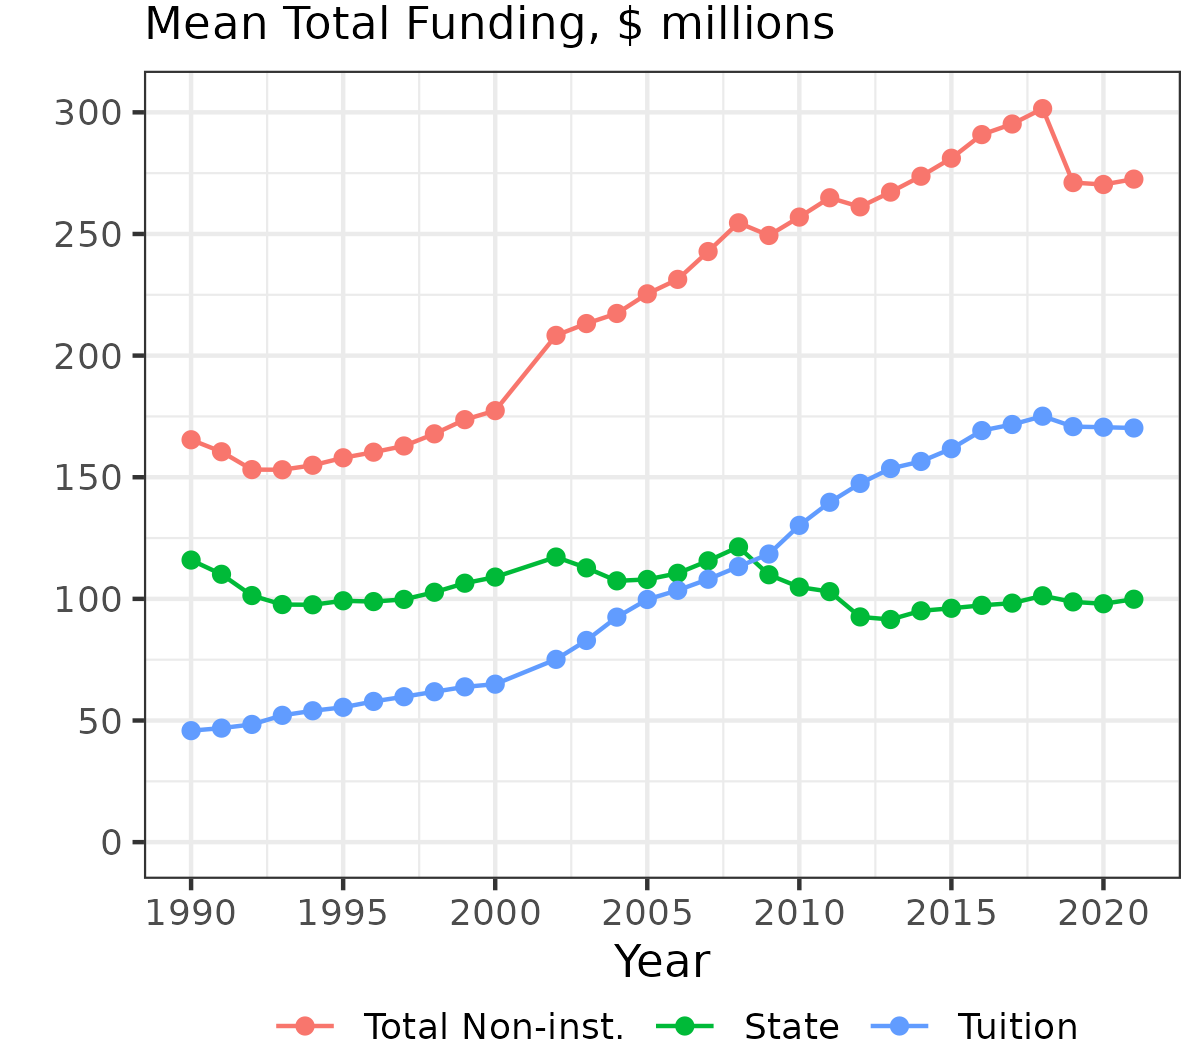
\includegraphics[width=\textwidth]{figures/mean-funding-total.png}
        \label{fig:mean-funding-total}
    \end{subfigure}
    \begin{subfigure}[b]{0.495\textwidth}
        \centering
        \caption{Per Student, \$ 2021 CPI-U.}
        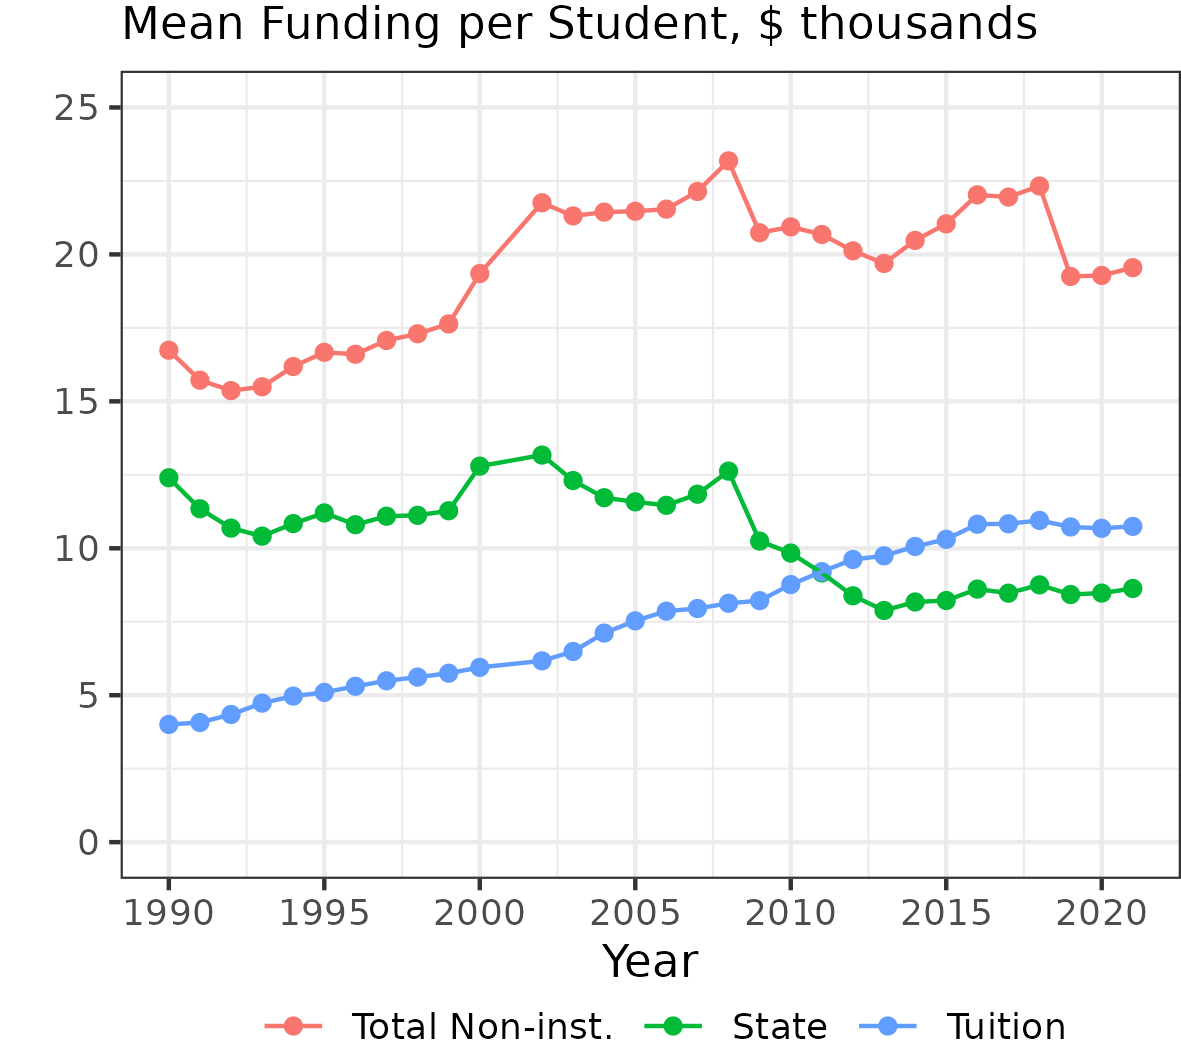
\includegraphics[width=\textwidth]{figures/mean-funding-fte.png}
        \label{fig:mean-funding-fte}
    \end{subfigure}
    \label{fig:funding}
    \justify
    \footnotesize
    \textbf{Note}:
    This figure shows the mean funding for US public universities as a total (in figure a.) and divided by student enrolment (figure b.).
    The numbers are adjusted to 2021 figures by CPI-U.
    Non-institutional revenues refers to the sum of federal, state, and local funding plus tuition revenues; these sum to the majority of university funding, but exclude numbers such as university income from capital projects.
    These figures are calculated with IPEDS data.
\end{figure}

\begin{figure}[H]
    \centering
    \singlespacing
    \caption{Total Student enrolment, by University Sector and Year.}
    \begin{subfigure}[b]{0.495\textwidth}
        \centering
        \caption{Total Enrolment, Nation-wide.}
        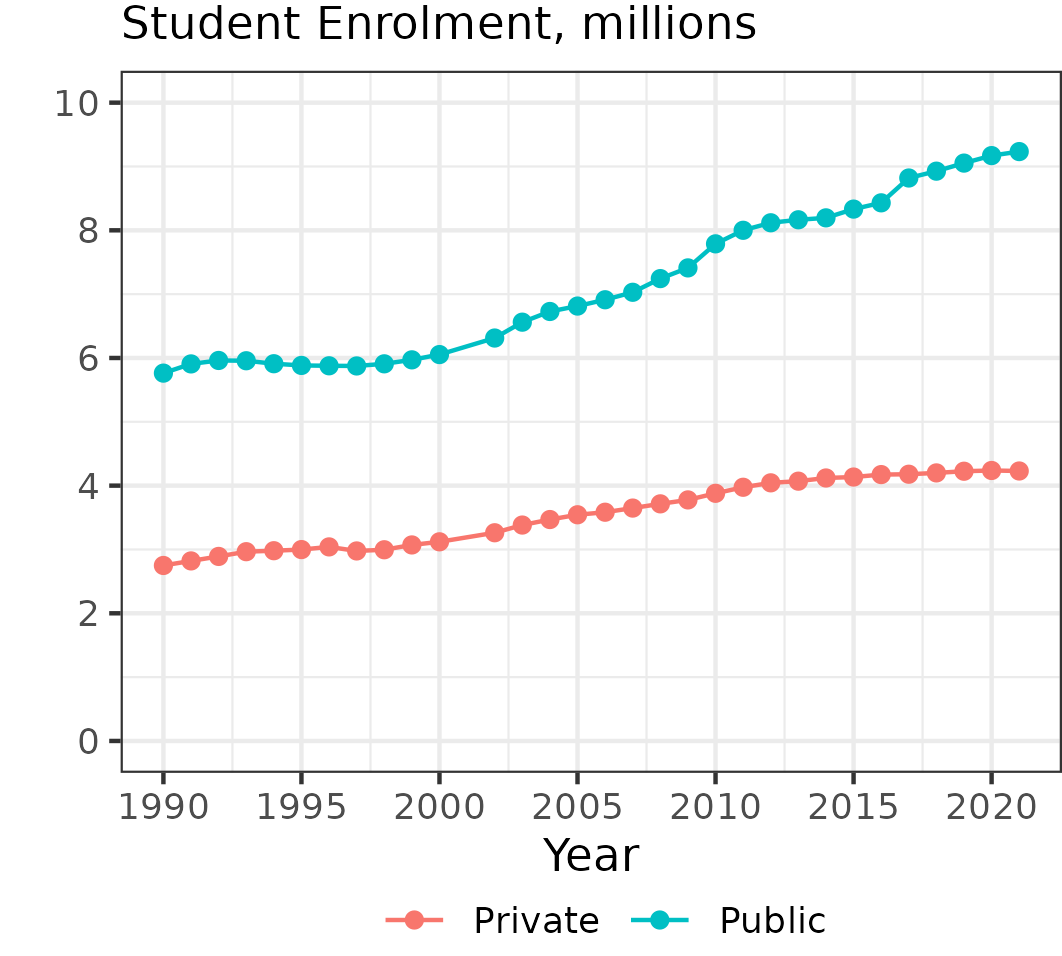
\includegraphics[width=\textwidth]{figures/enrollment-total.png}
        \label{fig:enrollment-total}
    \end{subfigure}
    \begin{subfigure}[b]{0.495\textwidth}
        \centering
        \caption{Mean Enrolment, per University.}
        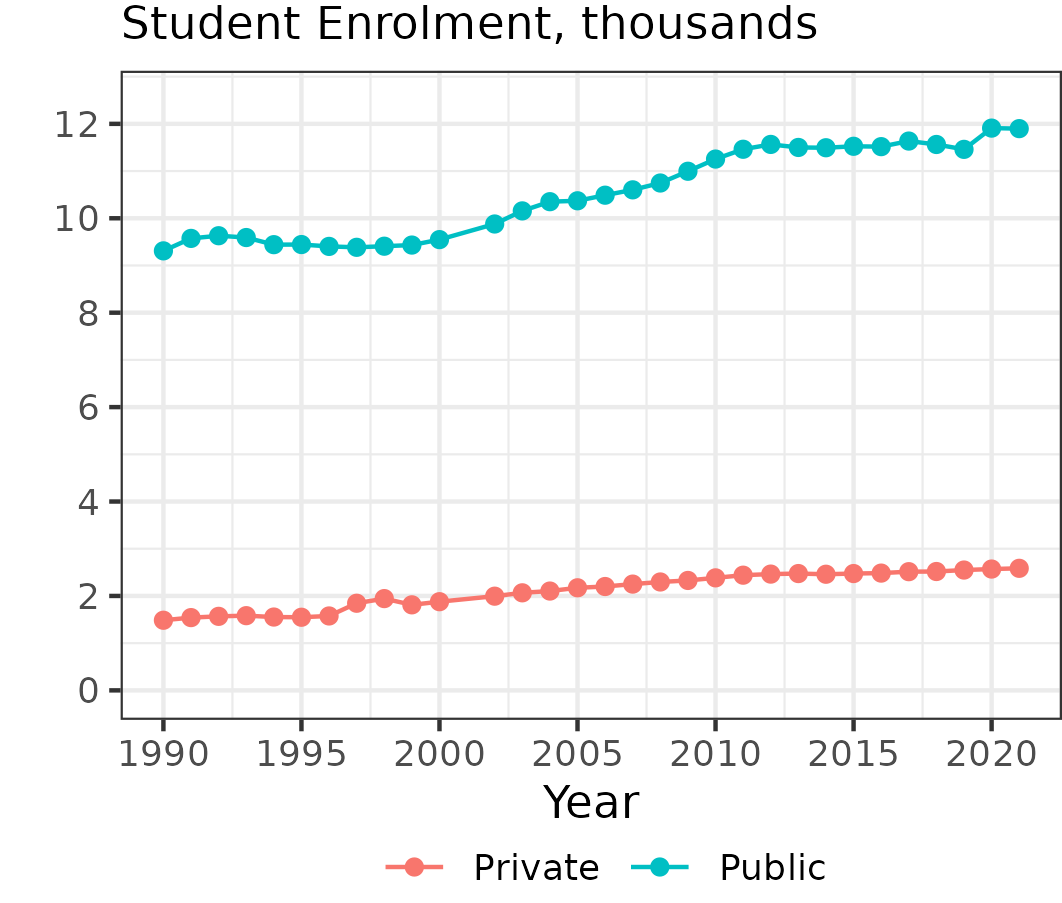
\includegraphics[width=\textwidth]{figures/enrollment-mean.png}
        \label{fig:enrollment-mean}
    \end{subfigure}
    \label{fig:enrolment}
    \justify
    \footnotesize
    \textbf{Note}:
    This figure shows the total and mean enrolment for US universities, comparing public and private universities.
    Most of the higher education enrolment increase for the last 30 years was in public universities, who continue to enrol the vast majority of higher education students in the US.
    These figures are calculated with IPEDS data.
\end{figure}

\newpage
\begin{figure}[H]
    \centering
    \singlespacing
    \caption{Trends in Mean Student Enrolment per Professor, by University Sector and Faculty level.}
    \begin{subfigure}[b]{0.495\textwidth}
        \centering
        \caption{Lecturer.}
        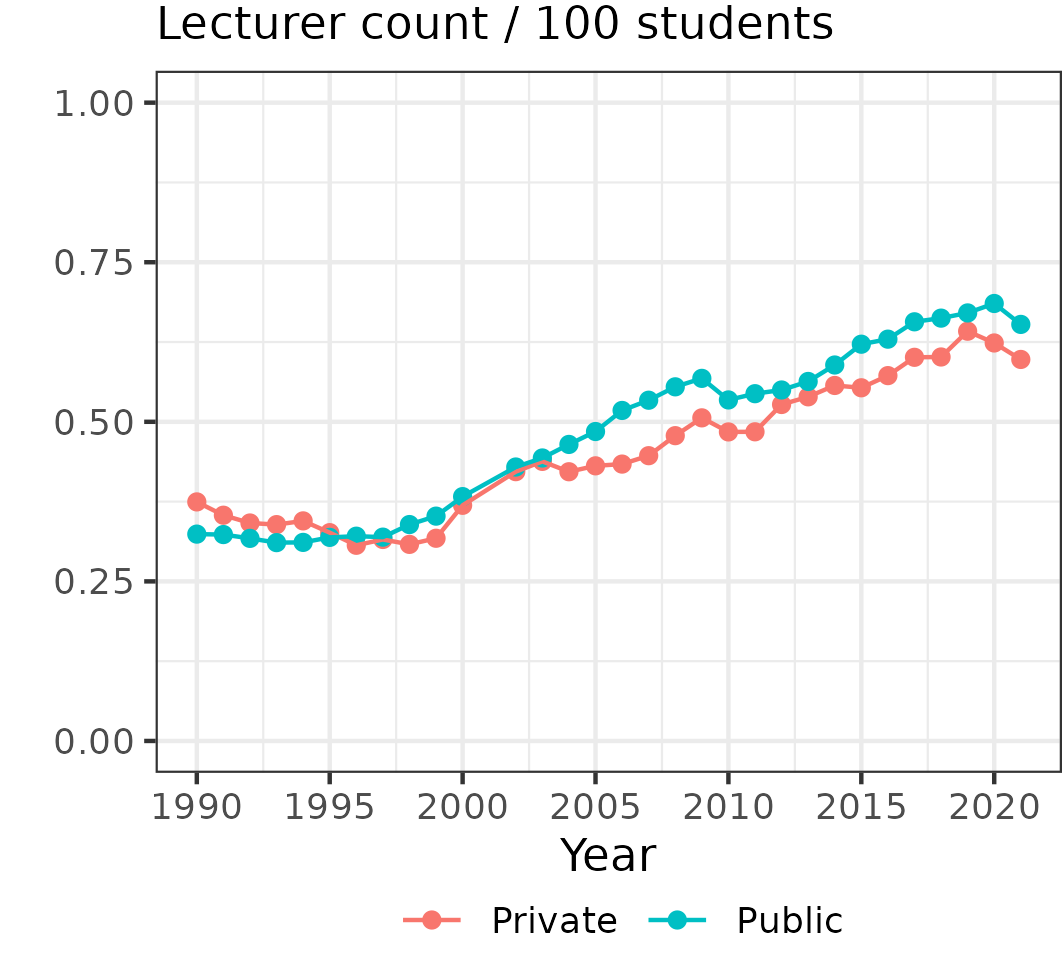
\includegraphics[width=\textwidth]{figures/lecturer-fte-perprof.png}
        \label{fig:lecturer-fte-perprof}
    \end{subfigure}
    \begin{subfigure}[b]{0.495\textwidth}
        \centering
        \caption{Assistant.}
        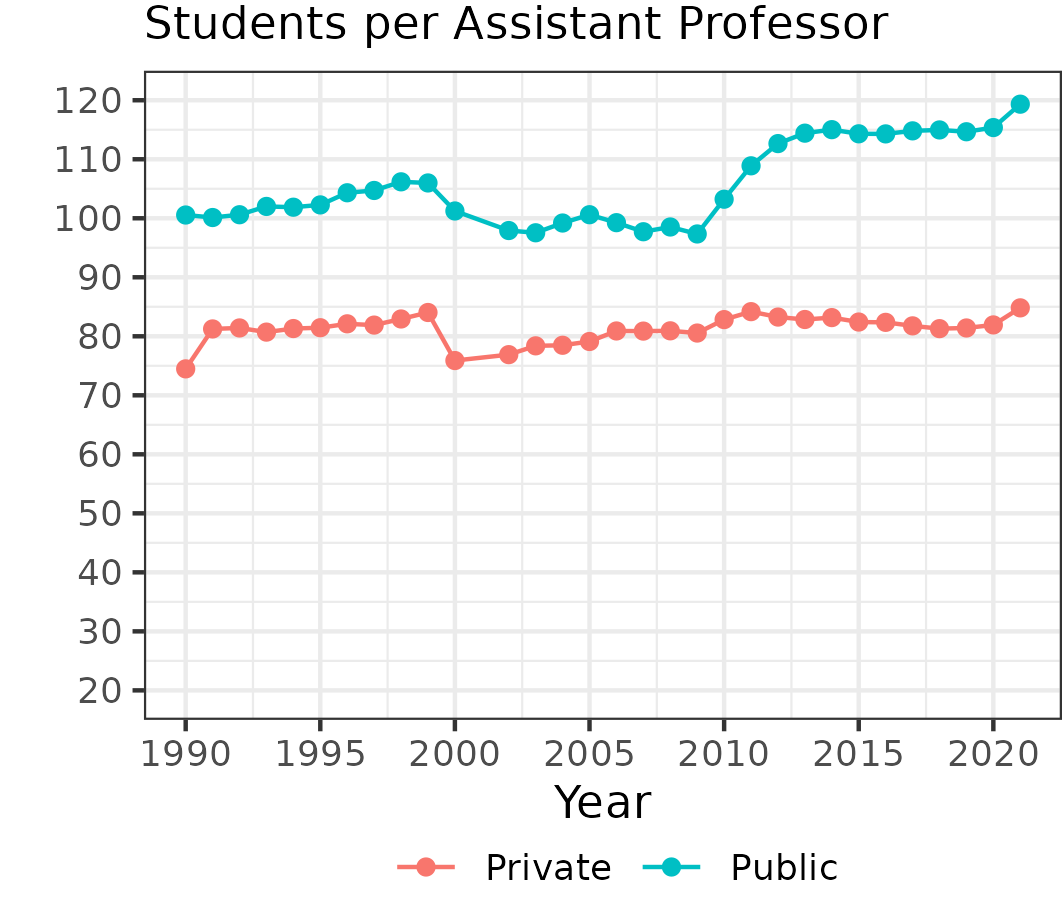
\includegraphics[width=\textwidth]{figures/assistant-fte-perprof.png}
        \label{fig:assistant-fte-perprof}
    \end{subfigure}
    \begin{subfigure}[b]{0.495\textwidth}
        \centering
        \caption{Full.}
        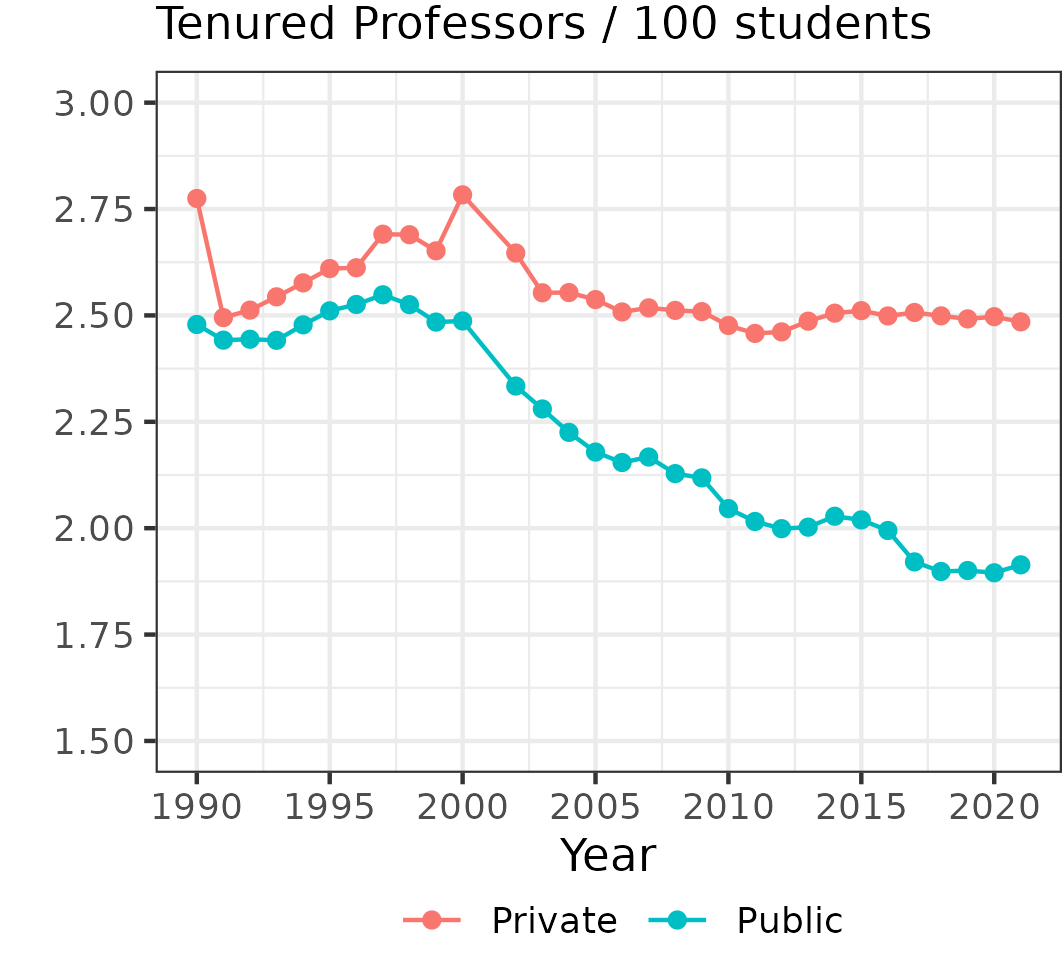
\includegraphics[width=\textwidth]{figures/full-fte-perprof.png}
        \label{fig:full-fte-perprof}
    \end{subfigure}
    \begin{subfigure}[b]{0.495\textwidth}
        \centering
        \caption{All.}
        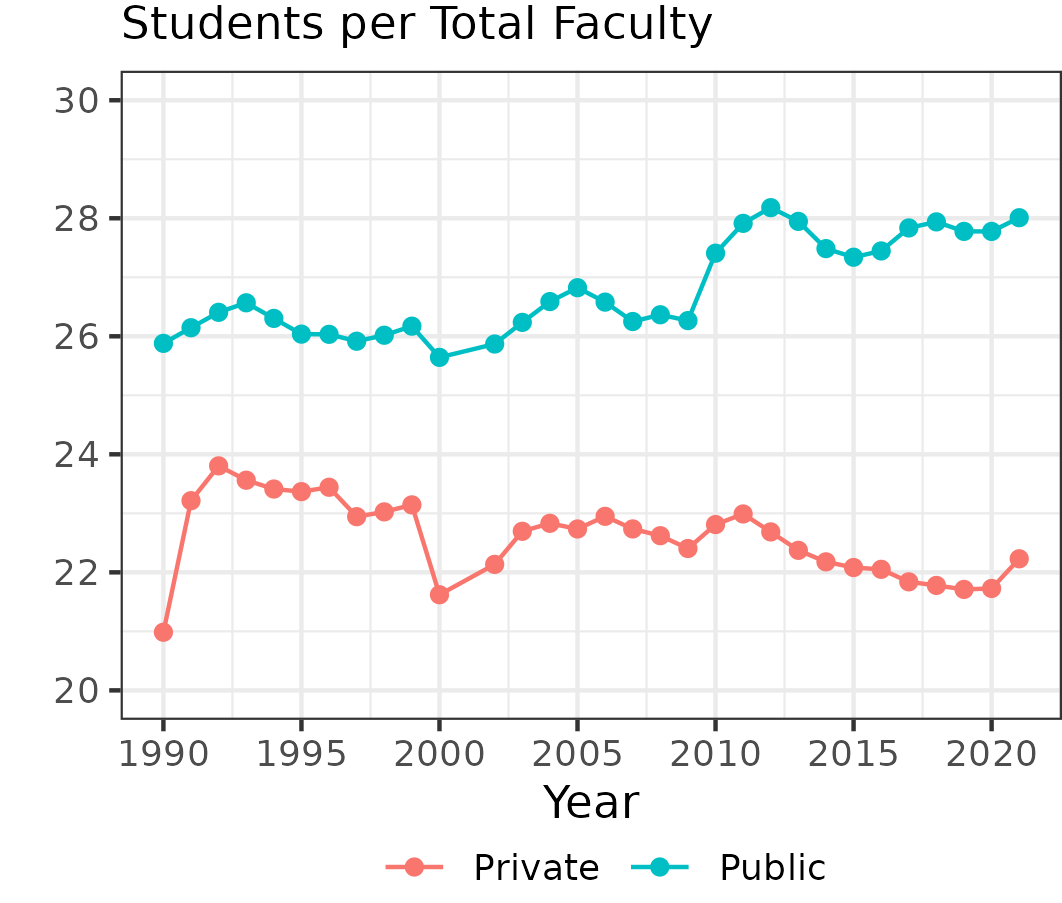
\includegraphics[width=\textwidth]{figures/all-fte-perprof.png}
        \label{fig:all-fte-perprof}
    \end{subfigure}
    \label{fig:fte-perprof}

    \justify
    \footnotesize
    \textbf{Note}:
    This figure shows the average number of students per faculty member, by different faculty position, at US public universities.
    E.g., panel A calculates the mean of (lecturer count) / (student enrolment) at US public universities, for each year of 1990--2017, to show the average trend in faculty composition compared to student enrolment.
    These figures are calculated with IPEDS data.
\end{figure}

\newpage
\begin{figure}[H]
    \centering
    \singlespacing
    \caption{Mean Funding Sources among Illinois Public Universities, by Year.}
    \begin{subfigure}[b]{0.495\textwidth}
        \centering
        \caption{Total, \$ 2021 CPI-U.}
        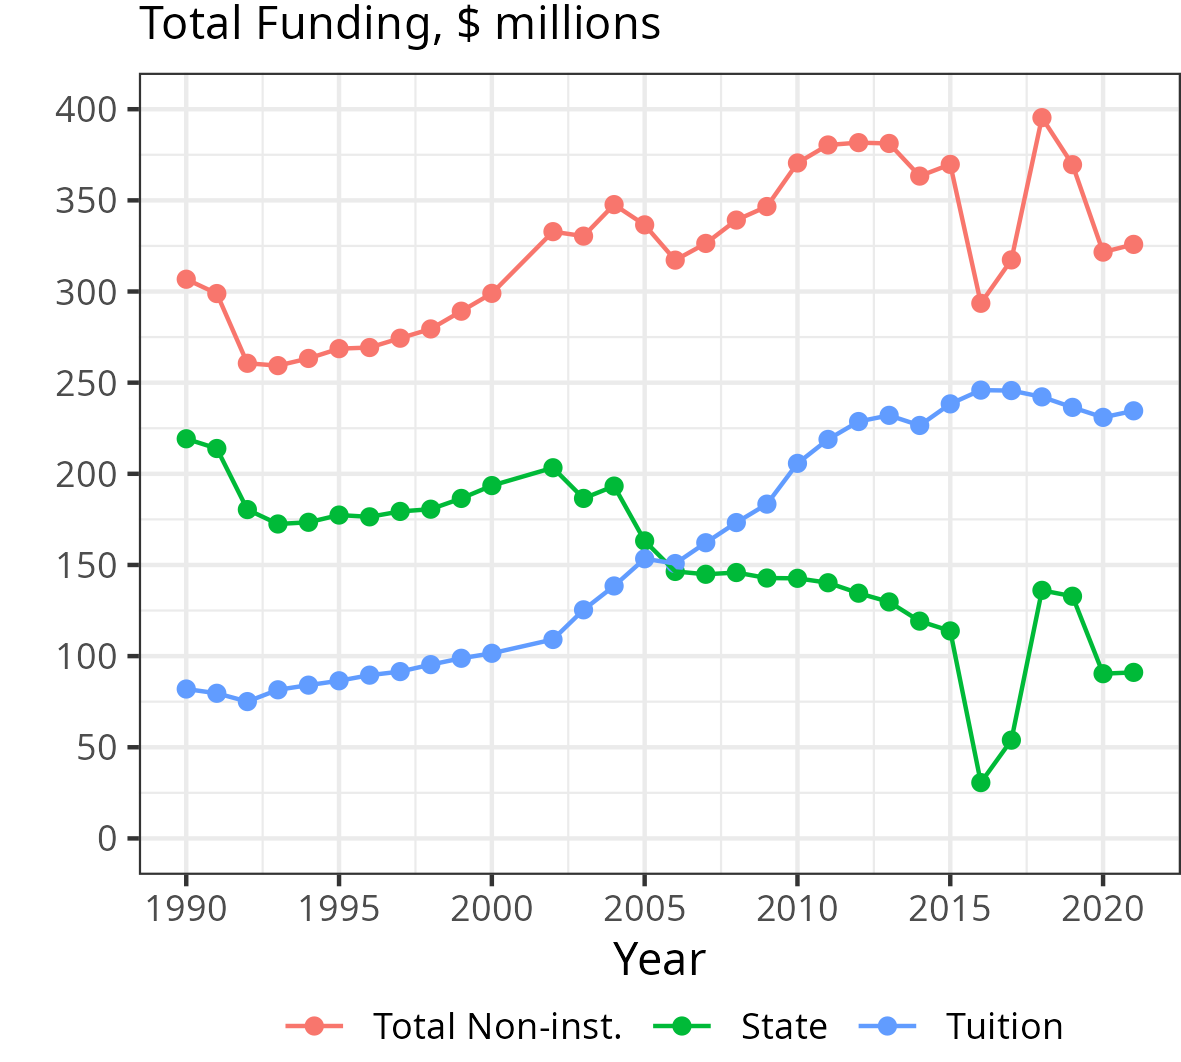
\includegraphics[width=\textwidth]{figures/illinois-funding-total.png}
        \label{fig:illinois-funding-total}
    \end{subfigure}
    \begin{subfigure}[b]{0.495\textwidth}
        \centering
        \caption{Per Student, \$ 2021 CPI-U.}
        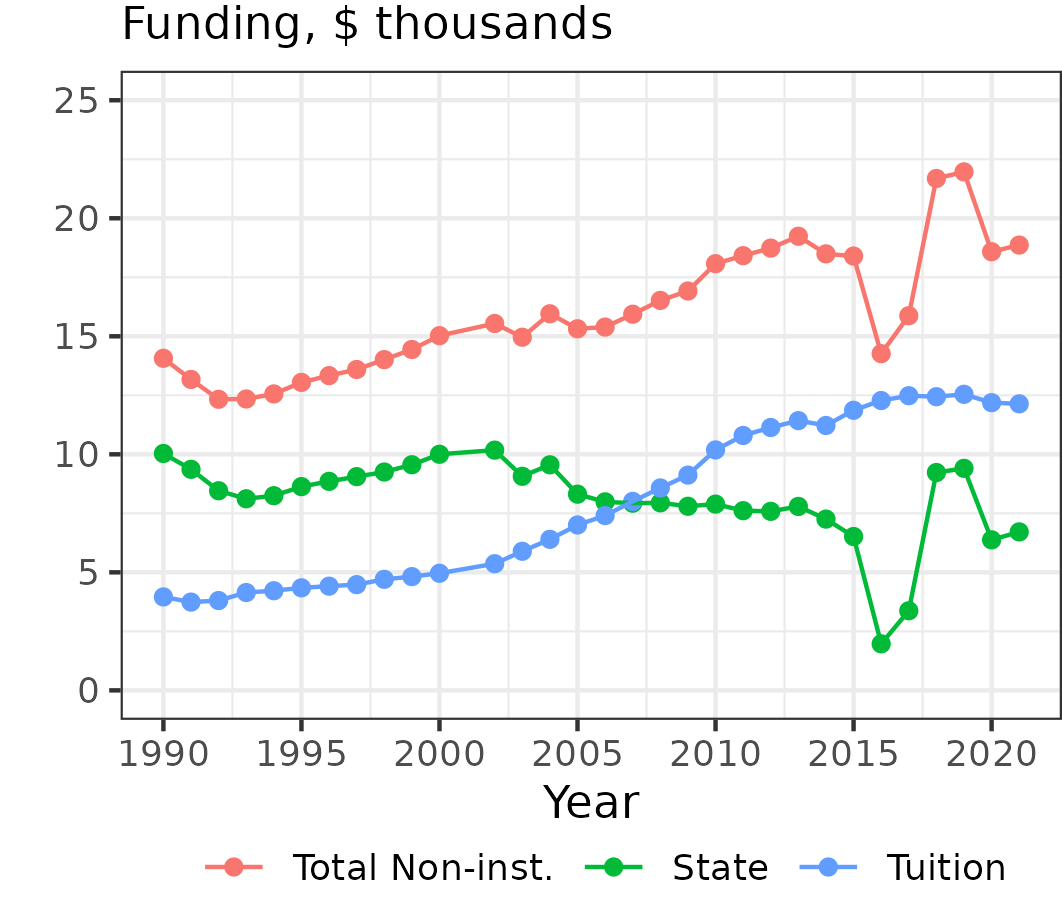
\includegraphics[width=\textwidth]{figures/illinois-funding-fte.png}
        \label{fig:illinois-funding-fte}
    \end{subfigure}
    \label{fig:illinois-funding}

    \justify
    \footnotesize
    \textbf{Note}:       
    This figure shows the mean funding for Illinois public universities as a total (in figure a.) and divided by student enrolment (figure b.).
    The numbers are adjusted to 2021 figures by CPI-U.
    Non-institutional revenues refers to the sum of federal, state, and local funding plus tuition revenues; these sum to the majority of university funding, but exclude numbers such as university income from capital projects.
    These figures are calculated with IPEDS data.
\end{figure}

\newpage
\begin{figure}[H]
    \centering
    \singlespacing
    \caption{Local Projection Estimates for Effect of State Funding on Faculty Count per Student at Universities, by Professor Group.}
    \begin{subfigure}[b]{0.495\textwidth}
        \centering
        \caption{Lecturers.}
        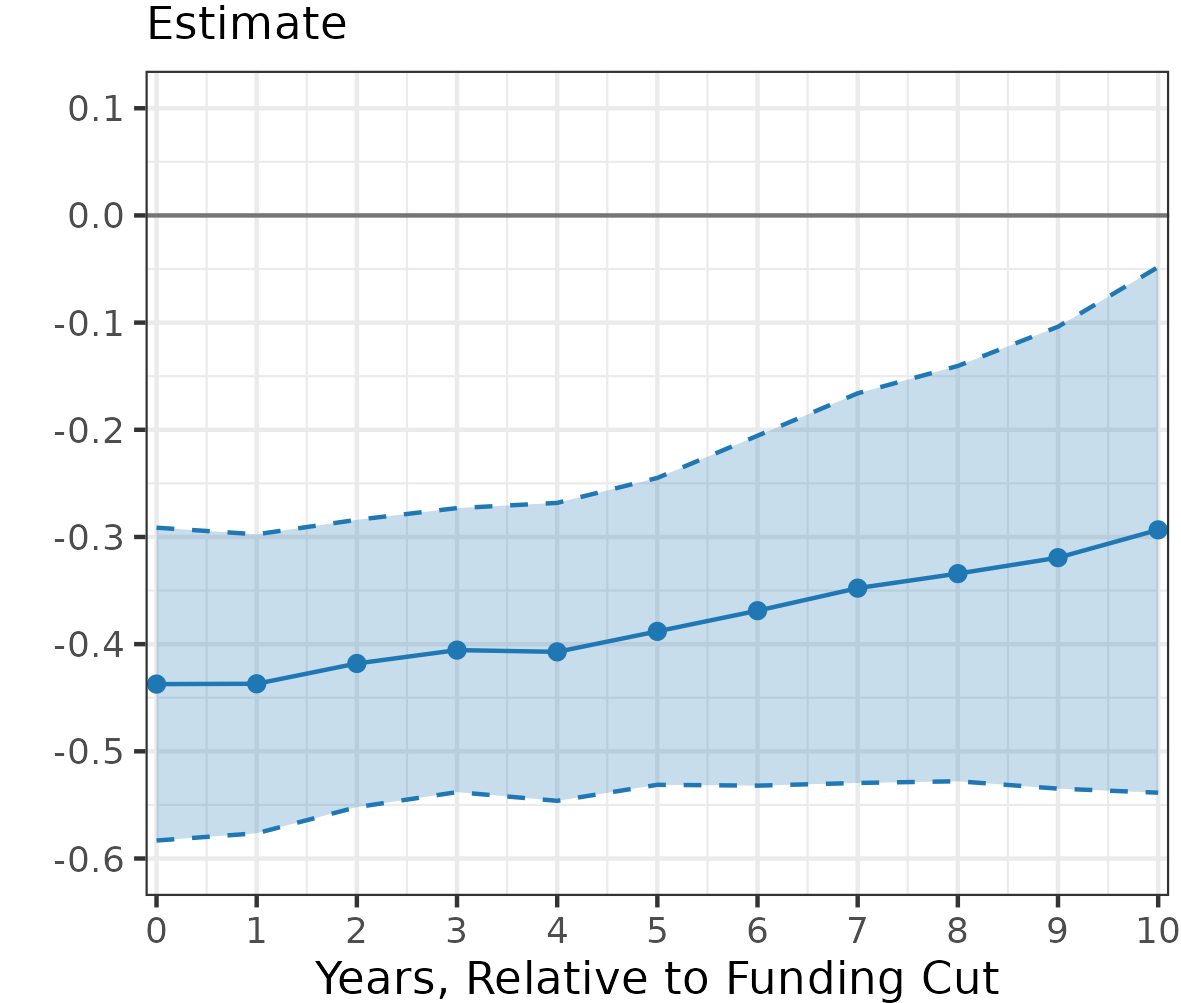
\includegraphics[width=\textwidth]{figures/lecturer-count-lp.png}
        \label{fig:lecturer-count-lp}
    \end{subfigure}
    \begin{subfigure}[b]{0.495\textwidth}
        \centering
        \caption{Assistant Professors.}
        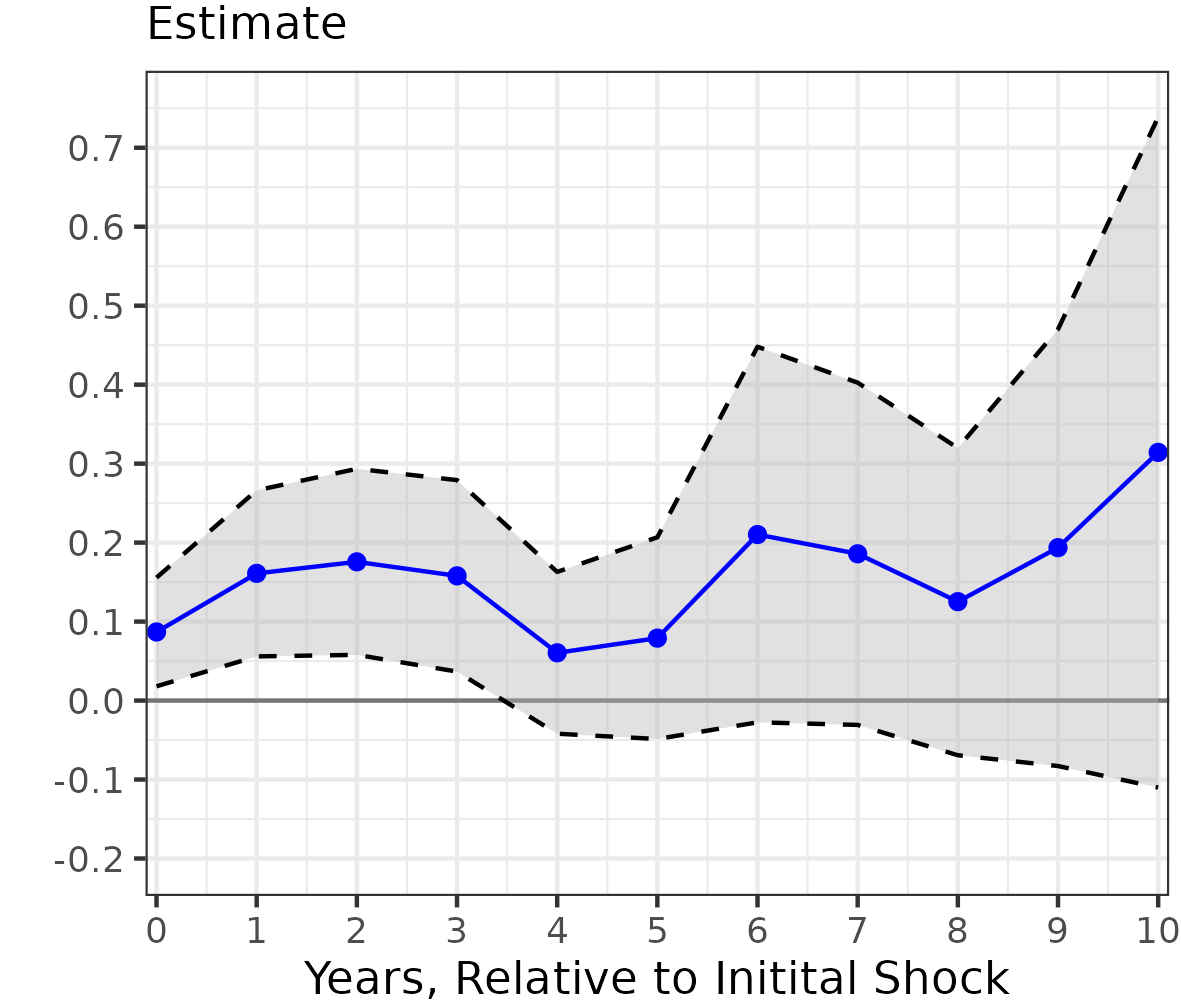
\includegraphics[width=\textwidth]{figures/assistant-count-lp.png}
        \label{fig:assistant-count-lp}
    \end{subfigure}
    \begin{subfigure}[b]{0.495\textwidth}
        \centering
        \caption{Full Professors.}
        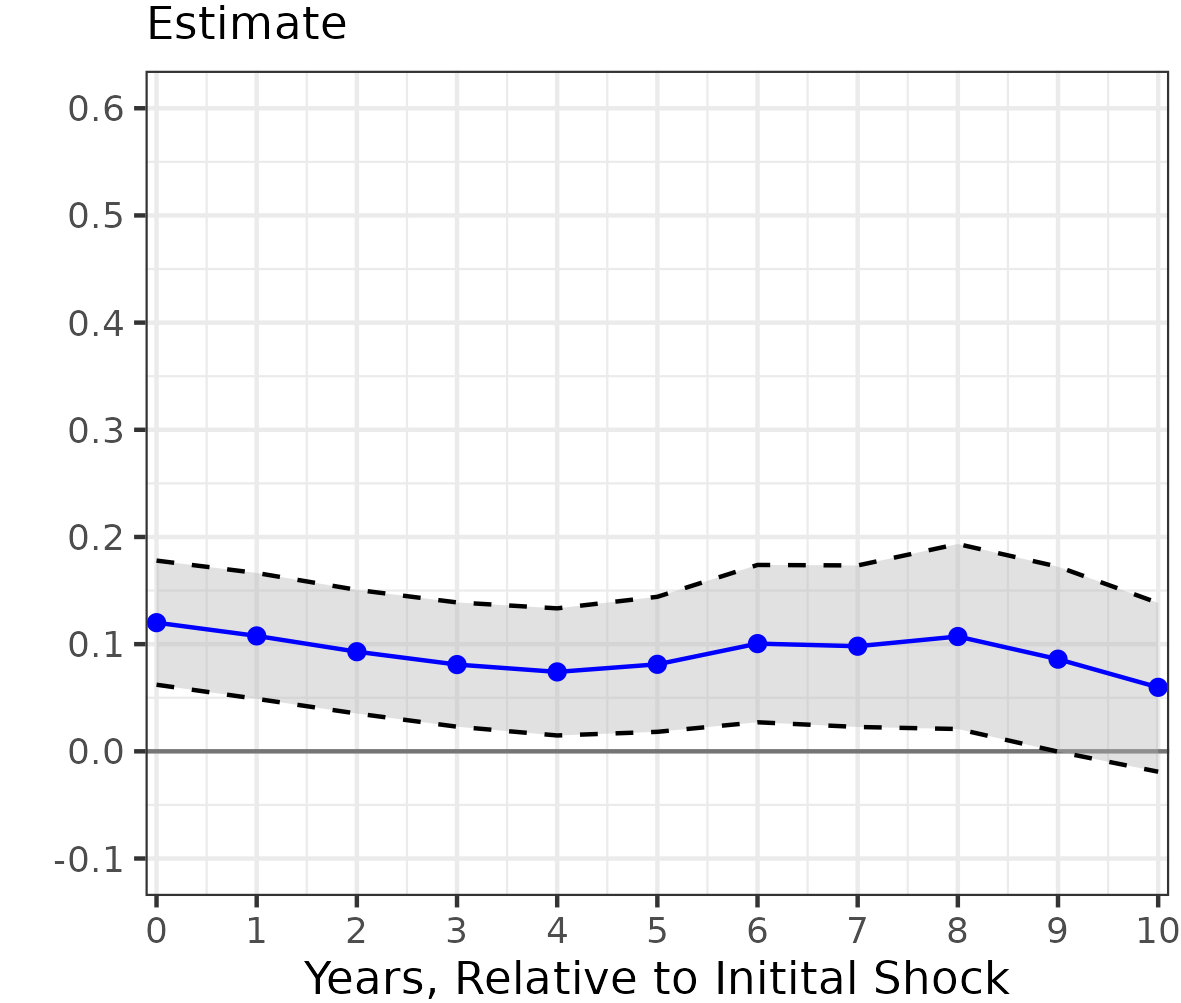
\includegraphics[width=\textwidth]{figures/full-count-lp.png}
        \label{fig:full-count-lp}
    \end{subfigure}
    \begin{subfigure}[b]{0.495\textwidth}
        \centering
        \caption{All Professors.}
        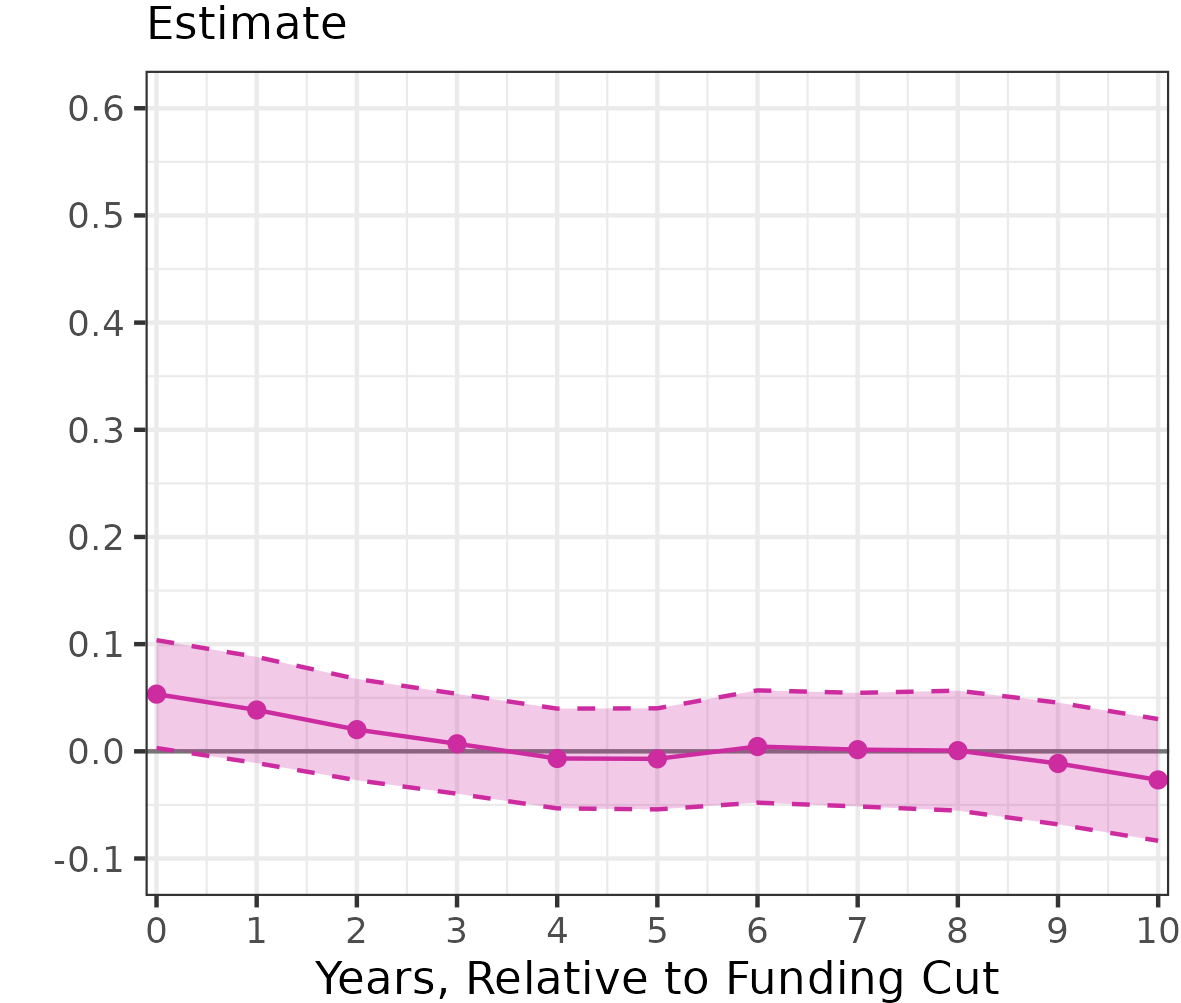
\includegraphics[width=\textwidth]{figures/all-count-lp.png}
        \label{fig:all-count-lp}
    \end{subfigure}
    \label{fig:count-lp}
    \justify
    \footnotesize
    \textbf{Note}:
    These figures show the local projections estimates of regression specification \eqref{eqn:secondstage}, with the funding shock as an instrument for state funding
    The unit of analysis is the university, and uses IPEDS data.
    The coefficient estimate is effect of state funding ($X_{i,t}$) on faculty count per student ($Y_{i,t}$), using the funding shock instrument ($Z_{i,t}$), while accounting for auto-correlation between different time periods --- i.e., between $X_{i,t}, X_{i,t-1}$ and $Y_{i,t}, Y_{i,t-1}$.
    These results use a $\log-\log$ specification, so the estimates are for the elasticity of professor count per student in a year $t+k$ with respect to state funding in year $t$, where years $k = 0, \hdots, 10$ are on the $x$-axis. 
    Standard errors are clustered at the state-year level.
\end{figure}

\newpage
\begin{figure}[H]
    \centering
    \singlespacing
    \caption{Local Projection Estimates for Effect of State Funding on Faculty Salaries per Student at Illinois Public Universities, by Professor Group.}
    \begin{subfigure}[b]{0.495\textwidth}
        \centering
        \caption{Lecturers.}
        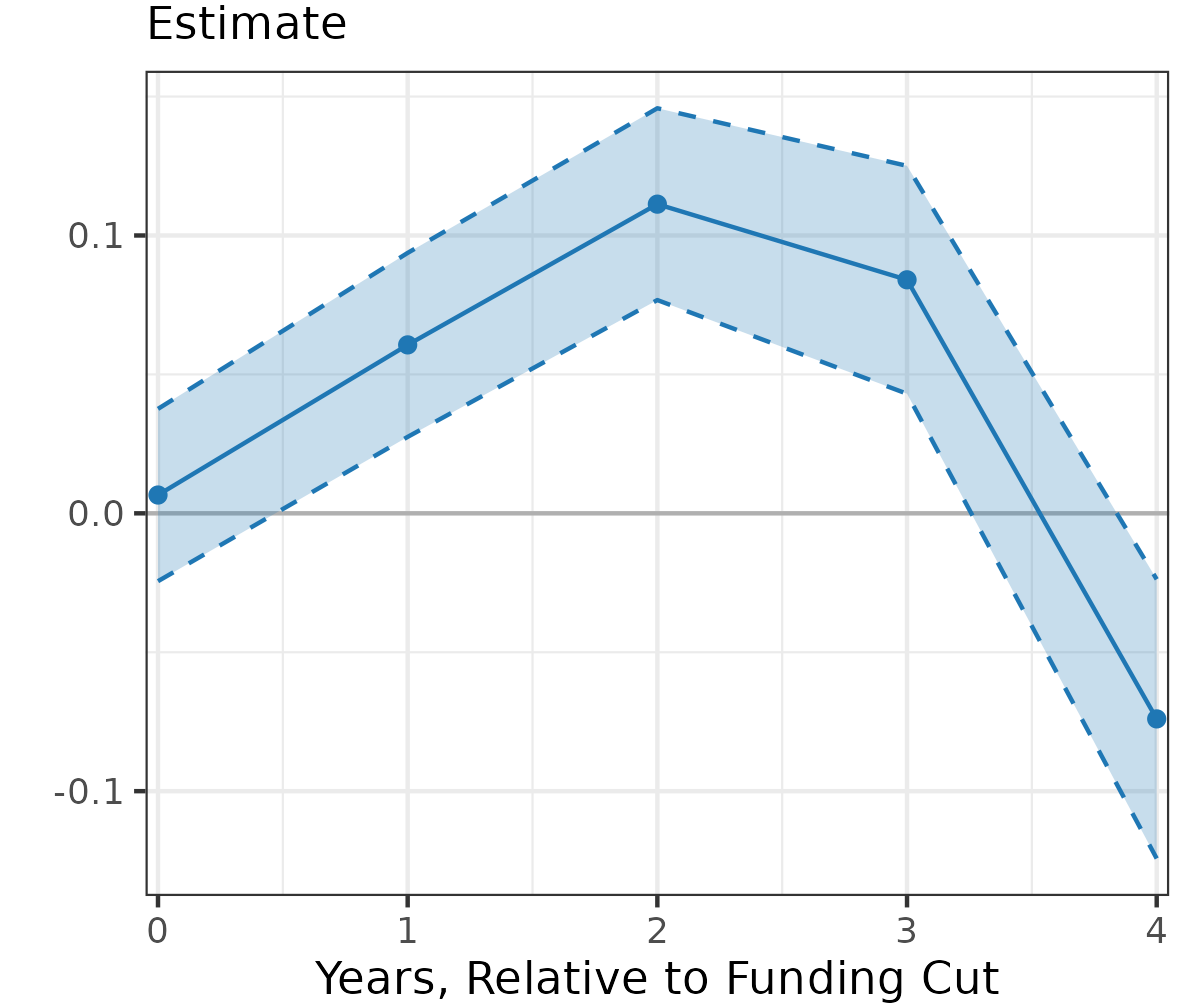
\includegraphics[width=\textwidth]{figures/salaries-lecturer-illinois-lp-rolling.png}
        \label{fig:salaries-lecturer-illinois-lp-rolling}
    \end{subfigure}
    \begin{subfigure}[b]{0.495\textwidth}
        \centering
        \caption{Assistant Professors.}
        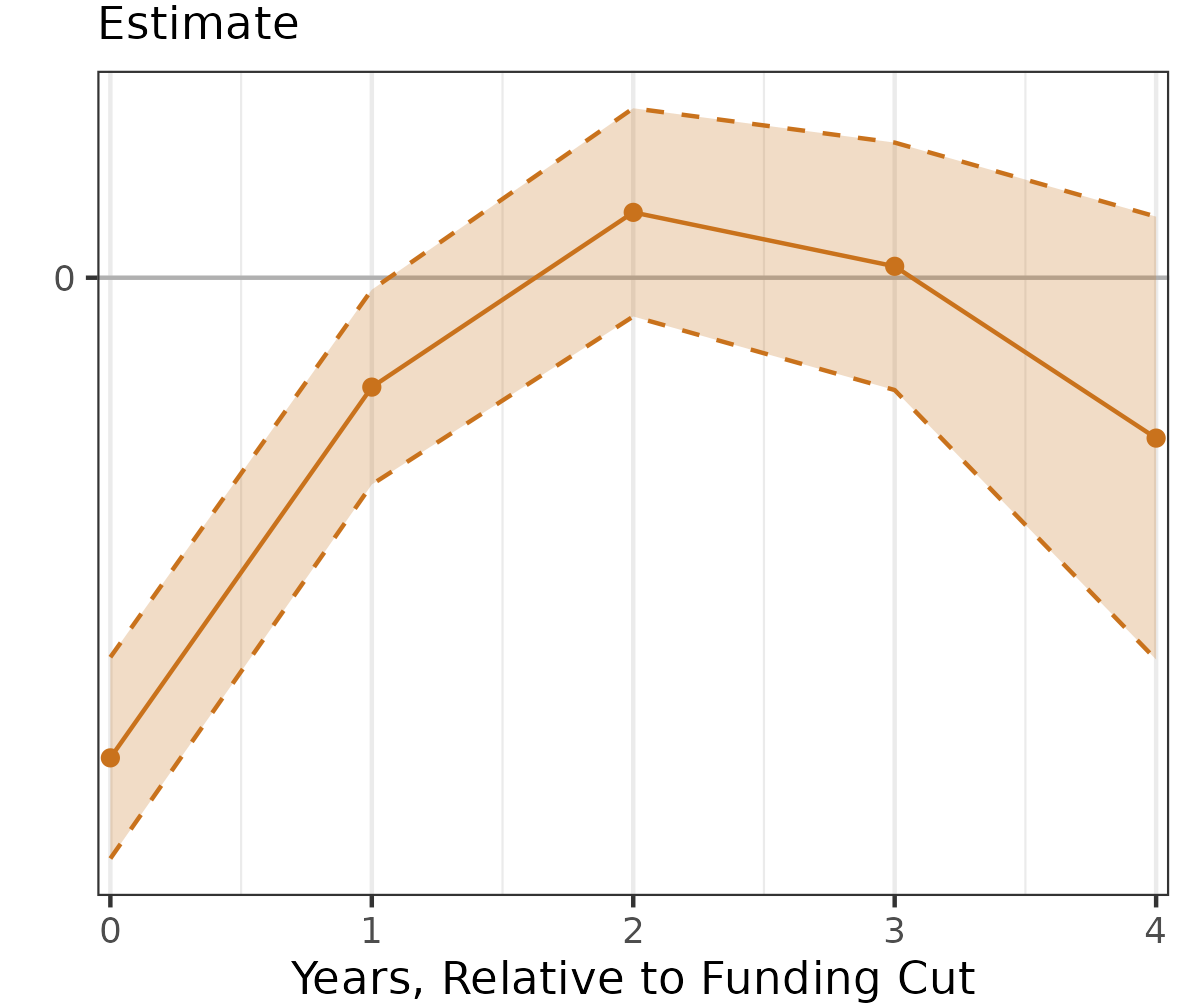
\includegraphics[width=\textwidth]{figures/salaries-assistant-illinois-lp-rolling.png}
        \label{fig:salaries-assistant-illinois-lp-rolling}
    \end{subfigure}
    \begin{subfigure}[b]{0.495\textwidth}
        \centering
        \caption{Full Professors.}
        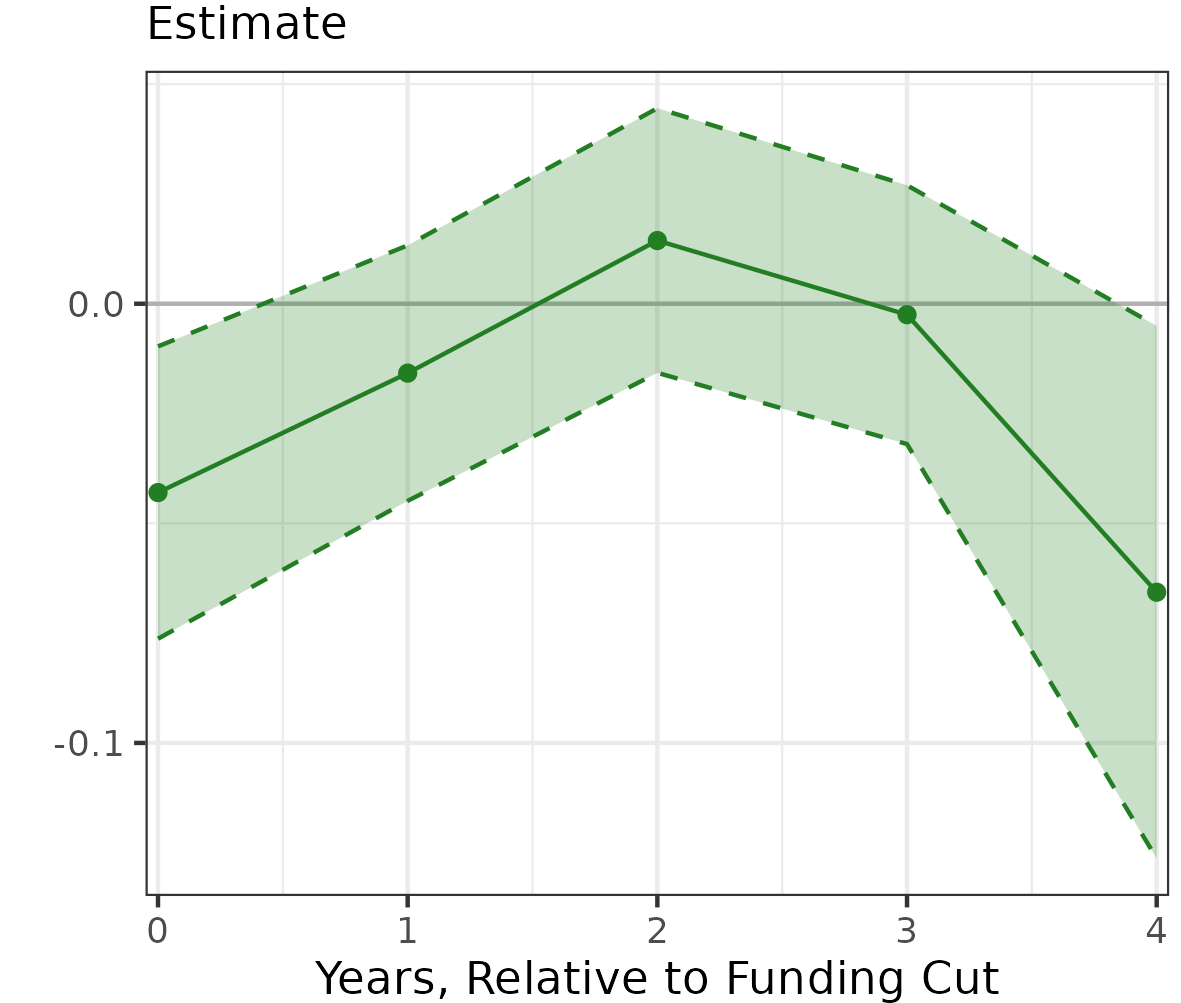
\includegraphics[width=\textwidth]{figures/salaries-full-illinois-lp-rolling.png}
        \label{fig:salaries-full-illinois-lp-rolling}
    \end{subfigure}
    \begin{subfigure}[b]{0.495\textwidth}
        \centering
        \caption{Administrator Professors.}
        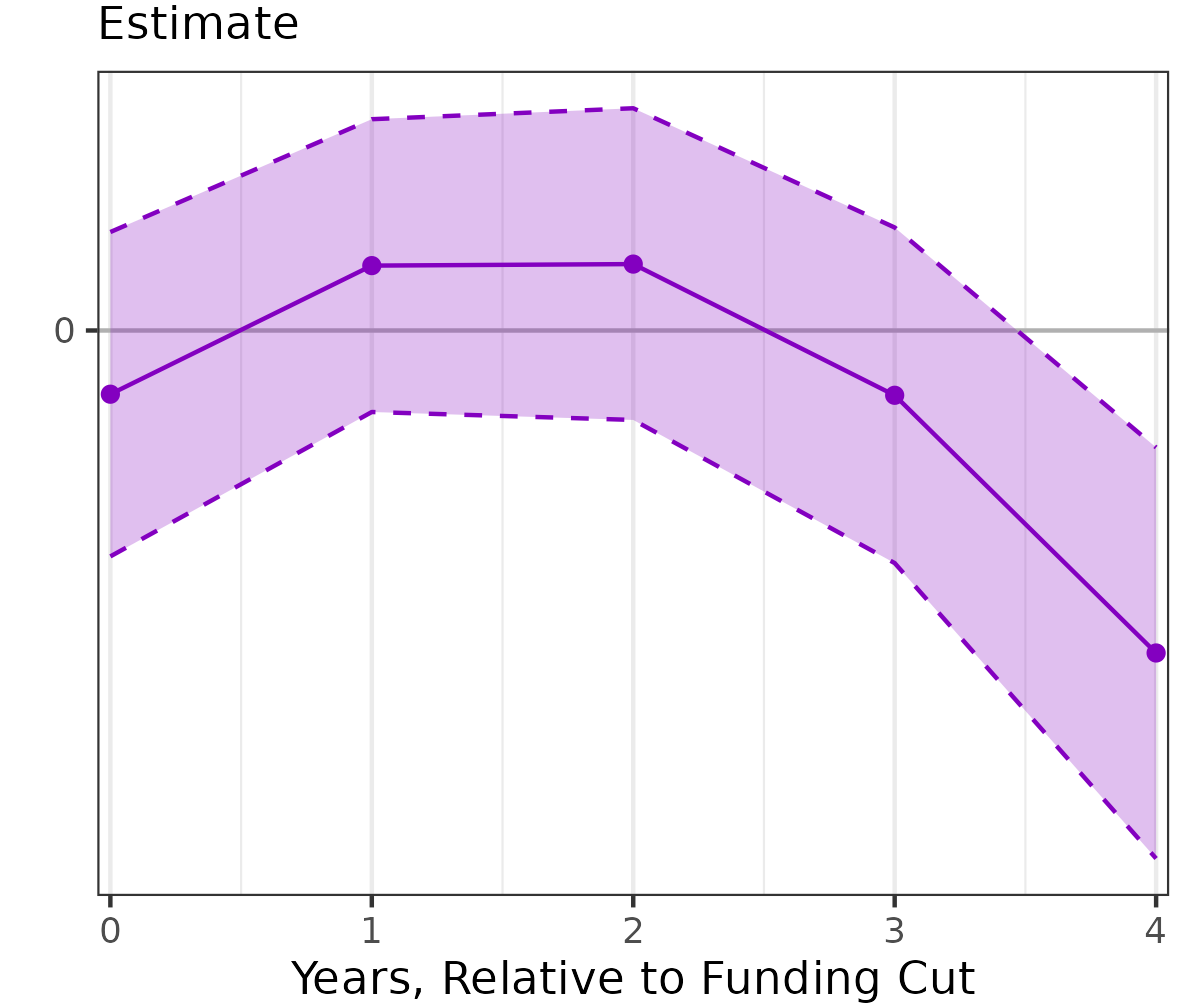
\includegraphics[width=\textwidth]{figures/salaries-administrator-illinois-lp-rolling.png}
        \label{fig:salaries-administrator-illinois-lp-rolling}
    \end{subfigure}
    \label{fig:salaries-illinois-lp-rolling}
    \justify
    \footnotesize
    \textbf{Note}:
    These figures show the local projections estimates of regression specification \eqref{eqn:secondstage}, with the funding shock as an instrument for state funding.
    The unit of analysis is an individual faculty member (at an Illinois public university); funding data come from IPEDS, and faculty salaries from IBHED.
    The coefficient estimate is effect of state funding ($X_{i(j),t}$) on faculty salaries ($Y_{j,t}$), using the funding shock instrument ($Z_{i(j),t}$), while accounting for auto-correlation between different time periods --- i.e., between $X_{i(j),t}, X_{i(j),t-1}$ and $Y_{i(j),t}, Y_{i(j),t-1}$.
    These results use a $\log-\log$ specification, so the estimates are for the elasticity of faculty salaries student in a year $t+k$ with respect to state funding in year $t$, where years $k = 0, \hdots, 4$ are on the $x$-axis. 
    Standard errors are clustered at the university-year level, and \autoref{sec:iv-model-indiv} fully describes the differences in empirical specification when unit of analysis is an individual faculty member.
\end{figure}


%%%%%%%%%%%%%%%%%%%%%%%%%%%%%%%%%%%%%%%%%
%% Section to host Tables
\newpage
\section{Tables}
\label{sec:tables}

\begin{table}[H]
    \singlespacing
    %\centering
    \caption{IPEDS Summary Statistics, Public Universities Panel 1990--2021}
    \makebox[\textwidth][c]{
\begin{tabular}{@{\extracolsep{5pt}}lccc} 
\\[-1.8ex]\hline 
\hline \\[-1.8ex] 
Statistic & \multicolumn{1}{c}{Mean} & \multicolumn{1}{c}{St. Dev.} & \multicolumn{1}{c}{N} \\ 
\hline \\[-1.8ex] 
Enrolment & 11,870 & 10,876 & 17,012 \\ 
State Funding (millions 2021 USD) & 104 & 127 & 17,012 \\ 
Total revenues (millions 2021 USD) & 450 & 818 & 17,012 \\ 
Non-institutional revenues (millions 2021 USD) & 213 & 272 & 17,012 \\ 
Lecturers count & 59 & 73 & 17,012 \\ 
Assistant professors count & 116 & 102 & 17,012 \\ 
Full professors count & 269 & 287 & 17,012 \\ 
All faculty count & 453 & 445 & 17,012 \\ 
\hline \\[-1.8ex] 
\end{tabular} 
}
    \label{tab:ipeds-summary}
    \justify
    \footnotesize
    \textbf{Note}:
    This table shows the summary statistics for every public university--year observation in IPEDS data.
    The numbers are adjusted to 2021 figures by CPI-U.
    Non-institutional revenues refers to the sum of federal, state, and local funding plus tuition revenues; these sum to the majority of university funding, but exclude numbers such as university income from capital projects.
\end{table}

\begin{table}[H]
    \singlespacing
    \centering
    \caption{IBHED Summary Statistics, Professor Panel 2010--2021.}
    \makebox[\textwidth][c]{
\begin{tabular}{@{\extracolsep{5pt}}lccc} 
\\[-1.8ex]\hline 
\hline \\[-1.8ex] 
Statistic & \multicolumn{1}{c}{Mean} & \multicolumn{1}{c}{St. Dev.} & \multicolumn{1}{c}{N} \\ 
\hline \\[-1.8ex] 
Lecturer, percent & 27 & 44 & 187,634 \\ 
Assistant professor, percent & 21 & 41 & 187,634 \\ 
Full professor, percent & 37 & 48 & 187,634 \\ 
Administrator professor, percent & 15 & 36 & 187,634 \\ 
Lecturer salary (2021 USD) & 31,449 & 25,786 & 50,588 \\ 
Assistant salary (2021 USD) & 76,897 & 38,059 & 39,421 \\ 
Full salary (2021 USD) & 109,283 & 48,919 & 68,774 \\ 
Administrator salary (2021 USD) & 119,249 & 61,321 & 28,851 \\ 
All salary (2021 USD) & 83,027 & 55,843 & 187,634 \\ 
Lecturer benefits (2021 USD) & 2,342 & 6,470 & 50,588 \\ 
Assistant benefits (2021 USD) & 2,965 & 7,096 & 39,421 \\ 
Full benefits (2021 USD) & 6,722 & 13,624 & 68,774 \\ 
Administrator benefits (2021 USD) & 3,599 & 15,928 & 28,851 \\ 
All benefits (2021 USD) & 4,272 & 11,513 & 187,634 \\ 
\hline \\[-1.8ex] 
\end{tabular} 
}
    \label{tab:illinois-summary}

    \justify
    \footnotesize
    \textbf{Note}:
    This table shows the summary statistics for every faculty--year observation in the IBHED data, which represents every faculty member in the Illinois public university system over years 2010--2021.
    The numbers are adjusted to 2021 figures by CPI-U.
    Lecturer is a binary for whether the faculty member is designated as a lecturer in the databse, and similarly for the assistant professors, full professors, and administrative faculty;
    salary refers the sum of base salary and benefits.
    All salary and benefits refers to summary statistics on the salary and benefits, respectively, of all faculty (regardless of position).
\end{table}

\newpage
\begin{table}[h!]
    \singlespacing
    \centering
    \caption{First Stage Estimates, for State Funding by funding shock.}
    \textbf{Panel A: units in \$ per student}
    
    \makebox[\textwidth][c]{
\begin{tabular}{@{\extracolsep{5pt}}lcccc} 
\\[-1.8ex]\hline 
\hline \\[-1.8ex] 
 & \multicolumn{4}{c}{Dependent Variable: State Funding} \\ 
\cline{2-5} 
\\[-1.8ex] & (1) & (2) & (3) & (4)\\ 
\hline \\[-1.8ex] 
 Funding Shock & $-$1.176 & $-$0.160 & $-$1.100 & $-$1.071 \\ 
  & (0.226) & (0.265) & (0.242) & (0.264) \\ 
  Tuition Revenue &  &  & $-$0.295 & 1.012 \\ 
  &  &  & (0.136) & (0.329) \\ 
  Constant &  & 9,716.437 &  & $-$1,708.334 \\ 
  &  & (1,805.394) &  & (2,716.150) \\ 
 \hline \\[-1.8ex] 
Uni. + Year fixed effects? & Yes & No & Yes & No \\ 
F stat. & 20.712 & 16.512 & 26.999 & 0.365 \\ 
Observations & 17,012 & 17,012 & 17,012 & 17,012 \\ 
R$^{2}$ & 0.918 & 0.0004 & 0.919 & 0.074 \\ 
\hline 
\hline \\[-1.8ex] 
\end{tabular} 
}
    
    \textbf{Panel B: units in log \$ per student}
    
    \makebox[\textwidth][c]{
\begin{tabular}{@{\extracolsep{5pt}}lcccc} 
\\[-1.8ex]\hline 
\hline \\[-1.8ex] 
 & \multicolumn{4}{c}{Dependent Variable: State Funding} \\ 
\cline{2-5} 
\\[-1.8ex] & (1) & (2) & (3) & (4)\\ 
\hline \\[-1.8ex] 
 Funding Shift-share& $-$0.977 & $-$0.302 & $-$0.986 & $-$0.573 \\ 
  & (0.066) & (0.093) & (0.062) & (0.067) \\ 
  Tuition Revenue &  &  & 0.058 & 0.535 \\ 
  &  &  & (0.059) & (0.065) \\ 
  Constant &  & 6.419 &  & $-$0.484 \\ 
  &  & (0.769) &  & (0.844) \\ 
 \hline \\[-1.8ex] 
Uni. + Year fixed effects? & Yes & No & Yes & No \\ 
F stat. & 249.662 & 74.022 & 218.171 & 10.558 \\ 
Observations & 17,012 & 17,012 & 17,012 & 17,012 \\ 
R$^{2}$ & 0.790 & 0.047 & 0.790 & 0.180 \\ 
\hline 
\hline \\[-1.8ex] 
\end{tabular} 
}
    
    \label{tab:firststage-reg}
    \justify
    \footnotesize
    \textbf{Note}:
    These tables show the first stage OLS estimates of regression specification \eqref{eqn:firststage}, showing the effect of the funding shock on state funding to gauge performance as an instrument.
    Each observation is a public univeristy-year, in the IPEDS data.
    Panel A shows the effect of an funding shock of \$-1 per student in the state on the number of \$'s of state funding per student at the university --- i.e.,
    \$-1 funding shock per student in the state leads to \$1.176 less state funding per student at the university according to preferred specification column 1.
    Panel B shows the effect of a $-10$\% change funding shock per student in the state on $10$\% change in state funding per student at the university --- i.e.,
    $-10$\% funding shock per student in the state leads to $-9.77$\% less state funding per student at the university according to prefferred specification column 1.        
    Standard errors are clustered at the state-year level, and univeristy $+$ year fixed effects are included where noted.
\end{table}

\newpage
\begin{table}[H]
    \singlespacing
    \centering
    \caption{Shift-Share Instrument Balance Test, in IPEDS 1990--2017.}

    \textbf{Panel A: units in \$}

    \makebox[\textwidth][c]{
\begin{tabular}{@{\extracolsep{5pt}}lcccccccc} 
\\[-1.8ex]\hline 
\hline \\[-1.8ex] 
 & \multicolumn{8}{c}{Dependent Variables: University Characteristics} \\ 
\cline{2-9}
\\[-1.8ex] & Enrolment & State & Total & Non-inst. &   & Assistant & Full & All \\ 
\\[-1.8ex] &           & Funding & Revenues & Revenues & Lecturers & Professors & Professors & Professors \\
\\[-1.8ex] & (1) & (2) & (3) & (4) & (5) & (6) & (7) & (8)\\ 
\hline \\[-1.8ex] 
 Funding & 0.517   & $-$9,217 & $-$7,633 & 886 & 0.007 & $-$0.001 & $-$0.003 & 0.004 \\ 
 Shock   & (0.199) & (2,452) & (12,771) & (4,093) & (0.002) & (0.001) & (0.003) & (0.005) \\ 
 \hline \\[-1.8ex] 
Uni. + Year \\
fixed effects? & Yes & Yes & Yes & Yes & Yes & Yes & Yes & Yes \\
Observations & 17,012 & 17,012 & 17,012 & 17,012 & 17,012 & 17,012 & 17,012 & 17,012 \\ 
R$^{2}$ & 0.960 & 0.950 & 0.881 & 0.932 & 0.745 & 0.886 & 0.973 & 0.954 \\ 
\hline 
\hline \\[-1.8ex] 
\end{tabular} 
}
    
    \textbf{Panel B: units in log \$ per student}
    
    \makebox[\textwidth][c]{
\begin{tabular}{@{\extracolsep{5pt}}lcccccccc} 
\\[-1.8ex]\hline 
\hline \\[-1.8ex] 
 & \multicolumn{8}{c}{Dependent Variables: University Characteristics} \\ 
\cline{2-9} 
\\[-1.8ex] & Enrolment & State Funding & Total revenues & Non-inst. revenues & Lecturers & Assistant professors & Full professors & All professors \\ 
\\[-1.8ex] & (1) & (2) & (3) & (4) & (5) & (6) & (7) & (8)\\ 
\hline \\[-1.8ex] 
 State Funding & 0.107 & $-$0.870 & 0.031 & $-$0.091 & 0.534 & $-$0.024 & $-$0.027 & 0.043 \\ 
  & (0.037) & (0.079) & (0.082) & (0.063) & (0.122) & (0.066) & (0.034) & (0.038) \\ 
 \hline \\[-1.8ex] 
Uni. + Year fixed effects? & Yes & Yes & Yes & Yes & Yes & Yes & Yes & Yes \\ 
Observations & 17,012 & 17,012 & 17,012 & 17,012 & 17,012 & 17,012 & 17,012 & 17,012 \\ 
R$^{2}$ & 0.976 & 0.914 & 0.979 & 0.975 & 0.782 & 0.902 & 0.963 & 0.965 \\ 
\hline 
\hline \\[-1.8ex] 
\end{tabular} 
}

    \justify
    \footnotesize
    \textbf{Note}:
    These tables show the OLS estimates of regression specification \eqref{eqn:firststage}, showing the effect of the funding shock on other outcomes to gauge balance of the instrument with respect to university characteristics
    Enrolment is measured in thousands of students.
    Each observation is a public univeristy-year, in the IPEDS data.
    Panel A shows the effect of an funding shock of \$$-1,000$ per student in the state on the counts of the outcome --- i.e.,
    \$$-1,000$ funding shock per student in the state is associated with 517 more students (as enrolment is measured in thousands) in column 1.
    Panel B shows the effect of a $-10$\% change funding shock per student in the state on $10$\% change in the outcomes --- i.e.,
    $-10$\% funding shock per student in the state is associated with an increase in 1.07\% more students at the unviersity according to prefferred column 1.        
    Standard errors are clustered at the state-year level, and univeristy $+$ year fixed effects are included where noted.
    \label{tab:firststage-balance}
\end{table}

\newpage
\begin{table}[H]
    \singlespacing
    \centering
    \caption{Effects of Changes in State Funding on University Faculty Composition, IPEDS 1990--2017, OLS and 2SLS Estimates.}

    \textbf{Panel A: units in \$ per student}

    \makebox[\textwidth][c]{
\begin{tabular}{@{\extracolsep{5pt}}lcccccccc} 
\\[-1.8ex]\hline 
\hline \\[-1.8ex] 
 & \multicolumn{8}{c}{Dependent Variable: Faculty Count per 1,000 Students, by Position} \\ 
\cline{2-9} 
\\[-1.8ex] & \multicolumn{2}{c}{Lecturers} & \multicolumn{2}{c}{Asst. Professors} & \multicolumn{2}{c}{Full Professors} & \multicolumn{2}{c}{All Faculty} \\ 
 & OLS & 2SLS & OLS & 2SLS & OLS & 2SLS & OLS & 2SLS \\ 
\\[-1.8ex] & (1) & (2) & (3) & (4) & (5) & (6) & (7) & (8)\\ 
\hline \\[-1.8ex] 
 State Funding & $-$0.451 & $-$5.957 & $-$0.479 & 1.031 & $-$0.104 & 2.288 & $-$1.198 & $-$3.333 \\ 
  & (0.177) & (1.725) & (0.211) & (1.232) & (0.275) & (2.910) & (0.612) & (4.259) \\ 
 \hline \\[-1.8ex] 
Outcome Mean & 59.253 & 59.253 & 116.121 & 116.121 & 269.103 & 269.103 & 452.507 & 452.507 \\ 
Observations & 17,012 & 17,012 & 17,012 & 17,012 & 17,012 & 17,012 & 17,012 & 17,012 \\ 
R$^{2}$ & 0.742 & 0.595 & 0.887 & 0.881 & 0.973 & 0.971 & 0.954 & 0.954 \\ 
\hline 
\hline \\[-1.8ex] 
\end{tabular} 
}
    
    \textbf{Panel B: units in log \$ per student}
    
    \makebox[\textwidth][c]{
\begin{tabular}{@{\extracolsep{5pt}}lcccccccc} 
\\[-1.8ex]\hline 
\hline \\[-1.8ex] 
 & \multicolumn{8}{c}{Dependent Variable: Employment Count by Professor Group} \\ 
\cline{2-9} 
\\[-1.8ex] & \multicolumn{2}{c}{Lecturer} & \multicolumn{2}{c}{Assistant} & \multicolumn{2}{c}{Full} & \multicolumn{2}{c}{All} \\ 
 & OLS & 2SLS & OLS & 2SLS & OLS & 2SLS & OLS & 2SLS \\ 
\\[-1.8ex] & (1) & (2) & (3) & (4) & (5) & (6) & (7) & (8)\\ 
\hline \\[-1.8ex] 
 State Funding & $-$0.137 & $-$0.437 & 0.082 & 0.135 & 0.123 & 0.137 & 0.077 & 0.065 \\ 
  & (0.032) & (0.100) & (0.047) & (0.068) & (0.056) & (0.038) & (0.047) & (0.030) \\ 
 \hline \\[-1.8ex] 
Outcome Mean & 0.572 & 0.572 & 1.194 & 1.194 & 2.298 & 2.298 & 4.128 & 4.128 \\ 
Observations & 17,012 & 17,012 & 17,012 & 17,012 & 17,012 & 17,012 & 17,012 & 17,012 \\ 
R$^{2}$ & 0.660 & 0.646 & 0.705 & 0.704 & 0.797 & 0.797 & 0.810 & 0.810 \\ 
\hline 
\hline \\[-1.8ex] 
\end{tabular} 
}

    \label{tab:facultycount-shock-reg}
    \justify
    \footnotesize
    \textbf{Note}:
    These tables show the second stage OLS and 2SLS estimates of regression specification \eqref{eqn:secondstage}, showing the effect of state funding changes on faculty outcomes, using the funding shock to instrument for state funding in the columns labelled 2SLS.
    Each observation is a public university-year, in the IPEDS data.
    Panel A shows the effect of a fall in state funding \$$-1,000$ per student in the state on the number of professors --- i.e.,
    an extra \$$1,000$ per student leads to 6 fewer lecturers according to column 2.
    Panel B shows the effect of a $10$\% change in state funding per student at the university on the 10\% change in the number of professors per students --- i.e.,
    an extra 10\% of state funding per student leads to 4.37\% fewer lecturers per student according to column 2.
    Outcome-mean is the mean of the outcome, for Panel A the number of professors per student, for Panel B the number of faculty per student.
    Panel B uses $\log$ faculty count per student as the outcome, though the outcome mean is count of faculty per student (not in $\log$ terms).
    Standard errors are clustered at the state-year level, and university $+$ year fixed effects are included through--out.
\end{table}


\newpage
\begin{table}[H]
    \singlespacing
    \centering
    \caption{Effects of Changes in State Funding on University Faculty Composition, in Illinois 2010--2021, OLS and 2SLS Estimates.}

    \textbf{Panel A: units in \$ per student}

    \makebox[\textwidth][c]{
\begin{tabular}{@{\extracolsep{5pt}}lcccccccc} 
\\[-1.8ex]\hline 
\hline \\[-1.8ex] 
 & \multicolumn{8}{c}{Dependent Variable: Employment Count by Professor Group} \\ 
\cline{2-9} 
\\[-1.8ex] & \multicolumn{2}{c}{Lecturer} & \multicolumn{2}{c}{Assistant} & \multicolumn{2}{c}{Full} & \multicolumn{2}{c}{All} \\ 
 & OLS & 2SLS & OLS & 2SLS & OLS & 2SLS & OLS & 2SLS \\ 
\\[-1.8ex] & (1) & (2) & (3) & (4) & (5) & (6) & (7) & (8)\\ 
\hline \\[-1.8ex] 
 State Funding & $-$3.729 & 0.376 & 0.415 & 3.208 & $-$1.269 & 0.117 & $-$4.084 & 3.890 \\ 
  & (1.721) & (1.725) & (1.728) & (2.493) & (1.548) & (1.200) & (4.352) & (5.668) \\ 
 \hline \\[-1.8ex] 
Outcome Mean & 351.306 & 351.306 & 273.757 & 273.757 & 477.597 & 477.597 & 1303.014 & 1303.014 \\ 
Observations & 144 & 144 & 144 & 144 & 144 & 144 & 144 & 144 \\ 
R$^{2}$ & 0.886 & 0.882 & 0.970 & 0.969 & 0.991 & 0.991 & 0.981 & 0.980 \\ 
\hline 
\hline \\[-1.8ex] 
\end{tabular} 
}
    
    \textbf{Panel B: units in log \$ per student}
    
    \makebox[\textwidth][c]{
\begin{tabular}{@{\extracolsep{5pt}}lcccccccc} 
\\[-1.8ex]\hline 
\hline \\[-1.8ex] 
 & \multicolumn{8}{c}{Dependent Variable: Employment Count by Professor Group} \\ 
\cline{2-9} 
\\[-1.8ex] & \multicolumn{2}{c}{Lecturer} & \multicolumn{2}{c}{Assistant} & \multicolumn{2}{c}{Full} & \multicolumn{2}{c}{All} \\ 
 & OLS & 2SLS & OLS & 2SLS & OLS & 2SLS & OLS & 2SLS \\ 
\\[-1.8ex] & (1) & (2) & (3) & (4) & (5) & (6) & (7) & (8)\\ 
\hline \\[-1.8ex] 
 State Funding & $-$0.015 & $-$0.017 & 0.049 & 0.058 & 0.007 & $-$0.029 & 0.004 & $-$0.008 \\ 
  & (0.033) & (0.026) & (0.045) & (0.038) & (0.021) & (0.032) & (0.028) & (0.022) \\ 
 \hline \\[-1.8ex] 
Outcome Mean & 2.523 & 2.523 & 1.491 & 1.491 & 2.729 & 2.729 & 8.141 & 8.141 \\ 
Observations & 144 & 144 & 144 & 144 & 144 & 144 & 144 & 144 \\ 
R$^{2}$ & 0.700 & 0.700 & 0.789 & 0.789 & 0.839 & 0.836 & 0.633 & 0.632 \\ 
\hline 
\hline \\[-1.8ex] 
\end{tabular} 
}

    \label{tab:facultycount-illinois-reg}
    \justify
    \footnotesize
    \textbf{Note}:
    These tables show the second stage OLS and 2SLS estimates of regression specification \eqref{eqn:secondstage}, showing the effect of state funding changes on number of faculty per student in Illinois universities, using the funding shock to instrument for state funding in the columns labelled 2SLS.
    Each observation is a public university-year in the state of Illinois, where funding data come from IPEDS and faculty count come from IBHED data.
    Panel A shows the effect of a fall in state funding \$$-1,000$ per student in the state on the number of professors.
    Panel B shows the effect of a $10$\% change in state funding per student at the university on the 10\% change in the number of professors per students.
    Outcome-mean is the mean of the outcome, for Panel A the number of professors per student, for Panel B the number of faculty per student.
    Panel B uses $\log$ faculty count per student as the outcome, though the outcome mean is count of faculty per student (not in $\log$ terms).
    Standard errors are clustered at the university-year level, and university $+$ year fixed effects are included through--out.
\end{table}

\newpage
\begin{table}[H]
    \singlespacing
    \centering
    \caption{Effects of Changes in State Funding on Faculty Salaries and Exit Rate, in Illinois 2010--2021, 2SLS Estimates.}
    \label{tab:faculty-shock-illinois-rolling}
    \makebox[\textwidth][c]{
\begin{tabular}{@{\extracolsep{5pt}}lccccc} 
\\[-1.8ex]\hline 
\hline \\[-1.8ex] 
 & \multicolumn{5}{c}{Dependent Variable: Annual Salaries} \\ 
\cline{2-6} 
 & Lecturer & Assistant & Full & Admin & All \\ 
\\[-1.8ex] & (1) & (2) & (3) & (4) & (5)\\ 
\hline \\[-1.8ex] 
 State Funding & 0.007 & $-$0.072 & $-$0.043 & $-$0.010 & $-$0.012 \\ 
  & (0.095) & (0.041) & (0.038) & (0.049) & (0.086) \\ 
 \hline \\[-1.8ex] 
Observations & 26,324 & 22,328 & 9,065 & 11,529 & 69,246 \\ 
R$^{2}$ & 0.220 & 0.051 & 0.069 & 0.144 & 0.163 \\ 
\hline 
\hline \\[-1.8ex] 
\end{tabular} 
}
    
    \makebox[\textwidth][c]{
\begin{tabular}{@{\extracolsep{5pt}}lccccc} 
\\[-1.8ex]\hline 
\hline \\[-1.8ex] 
 & \multicolumn{5}{c}{Dependent Variable: Exit rate by Professor Group} \\ 
\cline{2-6} 
 & Lecturer & Assistant & Full & Admin & All \\ 
\\[-1.8ex] & (1) & (2) & (3) & (4) & (5)\\ 
\hline \\[-1.8ex] 
 State Funding & $-$0.003 & 0.003 & $-$0.002 & $-$0.003 & $-$0.004 \\ 
  & (0.024) & (0.007) & (0.009) & (0.020) & (0.016) \\ 
 \hline \\[-1.8ex] 
Observations & 23,841 & 19,904 & 7,244 & 10,241 & 61,230 \\ 
R$^{2}$ & 0.013 & 0.005 & 0.013 & 0.072 & 0.016 \\ 
\hline 
\hline \\[-1.8ex] 
\end{tabular} 
}

    \makebox[\textwidth][c]{
\begin{tabular}{@{\extracolsep{5pt}}lcccc} 
\\[-1.8ex]\hline 
\hline \\[-1.8ex] 
 & \multicolumn{4}{c}{Dependent Variable: Promotion Rate by Professor Group} \\ 
\cline{2-5} 
 & Lecturer & Assistant & Associate & All \\ 
\\[-1.8ex] & (1) & (2) & (3) & (4)\\ 
\hline \\[-1.8ex] 
 State Funding & 0.015 & 0.036 & 0.029 & 0.016 \\ 
  & (0.007) & (0.019) & (0.065) & (0.008) \\ 
 \hline \\[-1.8ex] 
Observations & 16,420 & 16,972 & 4,340 & 42,132 \\ 
R$^{2}$ & 0.008 & 0.022 & 0.031 & 0.007 \\ 
\hline 
\hline \\[-1.8ex] 
\end{tabular} 
}

    \justify
    \footnotesize
    \textbf{Note}: 
    These tables show the second stage 2SLS estimates of regression specification \eqref{eqn:secondstage}, showing the effect of state funding changes on faculty outcomes at Illinois universities, using the funding shock to instrument for state funding.
    The shift-share instrument is based in the year the professor was hired, following definition in \autoref{sec:iv-model-indiv}.
    Each observation is a faculty member--year at an Illinois public university, where funding data come from IPEDS and faculty outcomes from IBHED data.
    The panels shows the effect of a $1$\% change in state funding per student at the university on faculties' salaries (base salary $+$ benefits), promotion rate (e.g., assistant professor to associate professor), and rate of leaving their university (i.e., by quitting, retiring, or moving to another university).
    Standard errors are clustered at the university-year of hire level, and university $+$ year of hire fixed effects are included through--out.
\end{table}


% Appendix
%%%%%%%%%%%%%%%%%%%%%%%%%%%%%%%%%%%%%%%%%
%% Appendix section
% Set-up the section.
\newpage
\appendix
\setcounter{table}{0}
\renewcommand{\thetable}{A\arabic{table}}
\setcounter{figure}{0}
\renewcommand{\thefigure}{A\arabic{figure}}

% Start appendix
\section{Appendix}
\label{appendix}
This project used data which are fully public, and computational tools which are fully open-source.
As such, all code and data (anonymised versions where necessary) involved in this project are available at this project's Github repository, available at \url{https://github.com/shoganhennessy/state-faculty-composition}.
They may be used for replication, or as the basis for further work, as needed.
Any comments or suggestions may be sent to me at \href{mailto:seh325@cornell.edu}{\nolinkurl{seh325@cornell.edu}}, or raised as an issue on the Github project.

A number of statistical packages, for the $R$ language \citep{R2022}, made the empirical analysis for this paper possible.
\begin{itemize}
    \item \textit{Tidyverse} \citep{tidyverse} collected tools for data analysis in the $R$ language.
    \item \textit{LFE} \citep{lfe} implemented linear fixed effect models, with instruments, crucial for the empirical estimation in \autoref{sec:empirics}.
    \item \textit{Stargazer} \citep{stargazer} provided methods to efficiently convert empirical results into presentable output in \LaTeX.
    \item \textit{Lpirfs} \citep{lpirfs2019} implemented estimation of the \cite{jorda2005} local projections methods, with instrumental variables, crucial to the local projections estimates presented in this project.
\end{itemize}

\subsection{IPEDS First Stage}
\label{sec:appendix-ipeds-firststage}

\begin{table}[H]
    \singlespacing
    \centering
    \caption{Shift-Share Instrument Balance, Mean Characteristics Across Instrument Distribution.}
    \makebox[\textwidth][c]{% latex table generated in R 4.3.3 by xtable 1.8-4 package
% Tue Sep 17 11:44:31 2024
\begin{tabular}{lccccc}
  \hline
Instrument Quantile: & 1st & 2nd & 3rd & 4th & 5th \\ 
  \hline
IV Components, \$ per student: &  &  &  &  &  \\ 
  Funding shift--share & -1,473.7 & -2,589.5 & -3,566.4 & -5,002.1 & -8,208.1 \\ 
  Shift in state--wide funding & -6,138.0 & -7,111.6 & -8,593.2 & -10,575.5 & -14,017.6 \\ 
  Share reliance on state funding, \% in 1990--1993 & 25.7 & 37.8 & 42.4 & 47.9 & 59.0 \\ 
  \hline University Funding and Spending, \$ millions: &  &  &  &  &  \\ 
  State funding & 110.3 & 99.2 & 99.8 & 107.1 & 107.1 \\ 
  Tuition revenue & 216.5 & 124.2 & 93.2 & 77.0 & 58.0 \\ 
  Total non-inst. revenues & 355.4 & 241.0 & 203.4 & 190.8 & 169.6 \\ 
  Instruction spending & 219.0 & 139.4 & 108.1 & 100.8 & 92.9 \\ 
  Research Spending & 150.0 & 74.6 & 53.9 & 35.9 & 25.5 \\ 
  \hline University Funding and Spending, \$ per student &  &  &  &  &  \\ 
  State funding & 12,900.1 & 9,956.2 & 9,334.7 & 9,304.9 & 12,766.7 \\ 
  Tuition revenue & 13,129.7 & 8,530.4 & 6,874.6 & 6,046.5 & 5,507.4 \\ 
  Total non-inst. revenues & 30,501.7 & 20,393.8 & 17,194.5 & 15,876.6 & 18,822.8 \\ 
  Instruction spending & 21,680.2 & 12,526.0 & 9,798.1 & 8,482.0 & 9,953.2 \\ 
  Research spending & 16,750.0 & 5,092.8 & 3,327.7 & 2,226.0 & 2,432.4 \\ 
  \hline Selectivity: &  &  &  &  &  \\ 
  Reported enrolment & 14,087.6 & 12,433.8 & 11,328.8 & 11,546.2 & 10,252.9 \\ 
  Full-time equivalent enrolment & 12,452.8 & 10,597.3 & 9,638.4 & 9,876.6 & 8,554.9 \\ 
  Acceptance rate, \% & 70.7 & 73.2 & 70.8 & 64.5 & 60.2 \\ 
  6 Year graduation rate, \% & 55.6 & 47.3 & 44.1 & 44.7 & 45.2 \\ 
   \hline
\end{tabular}
}
    \label{tab:summary-quantiles}
    \justify
    \footnotesize
    \textbf{Note}:
    This table shows the summary statistics for every public university--year observation in IPEDS data, for each of the 5 quantiles of the funding shift-share instrument.
    Funding shift-share is the instrument defined in \autoref{sec:empirics} the product of (1) state-wide funding shift and (2) share reliance on state funding.
    State-wide funding shift is total funding for higher education in that university's state (divided by the count of state students); share reliance on state funding is the the total amount of state funding received by the university in 1990--1993 divided by total revenues for those years. 
    The column labelled ``1st'' refers to the mean for all university-year observations in the first quintile (bottom 20\%) of the funding shift-share distribution, and so on.
    The numbers are adjusted to 2021 figures by CPI-U.
    Non-institutional revenues refers to the sum of federal, state, and local funding plus tuition revenues; these sum to the majority of university funding, but exclude numbers such as university income from capital projects.
    Acceptance rate and 6 year graduation rate are for university undergraduates, and are calculated from IPEDS data available for academic years 1997 through 2018.
\end{table}

\begin{figure}[H]
    \centering
    \singlespacing
    \caption{Correlation Between State Funding Shift-Share and Public University State Funding in Surrounding Years.}
    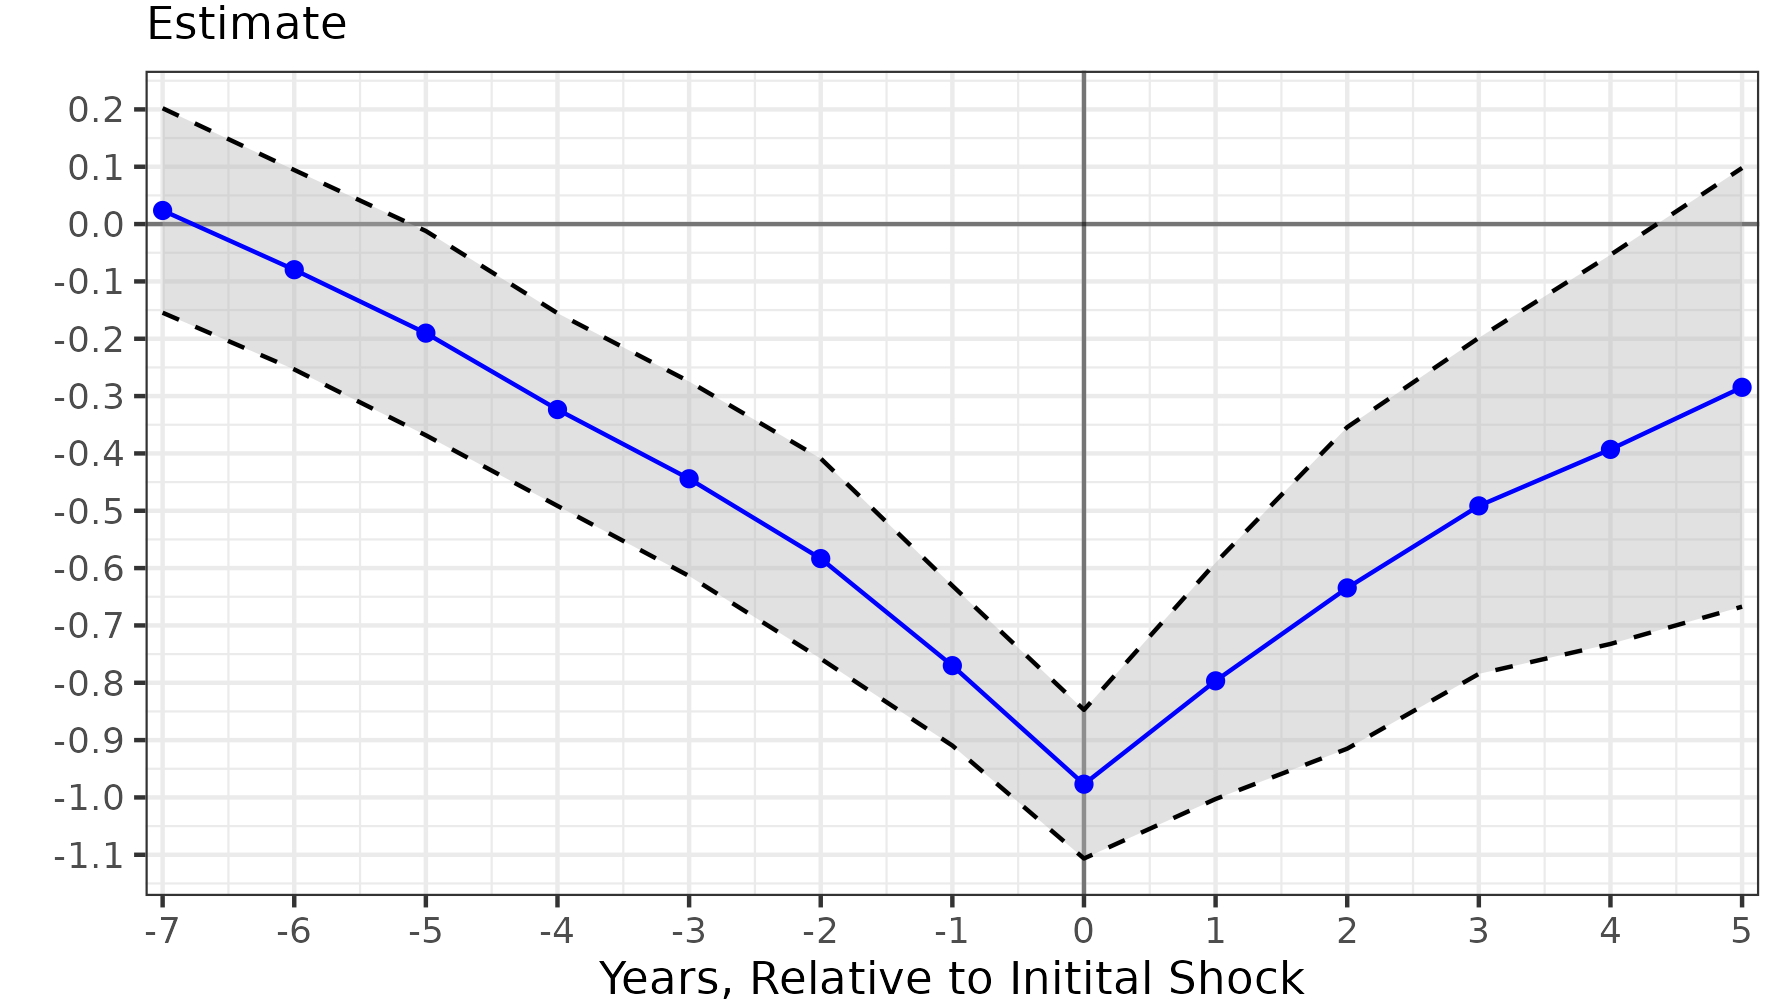
\includegraphics[width=\textwidth]{figures/lag-firststage.png}
    \label{fig:lag-firststage}
    \justify
    \footnotesize
    \textbf{Note}:
    This figure shows the correlation between state funding in year $t+k$ with the funding shift-share in year $t$ for a university, where $k = -7, \hdots, 5$ are the years on the $x$-axis.
    This shows that state funding and the funding shift-share are correlated across years, so that dynamic effects must be estimated by local projections --- and not simple OLS or 2SLS.
    The estimates are of \eqref{eqn:firststage}, calculated with IPEDS data, separately for each year relative to initial shock, using the $\log-\log$ specification, including fixed effects for university $+$ year, and clustering standard errors by university $+$ year.
\end{figure}

\begin{figure}[H]
    \centering
    \singlespacing
    \caption{Local Projection Estimates for Funding Shift-Share on State Funding, in IPEDS Data.}
    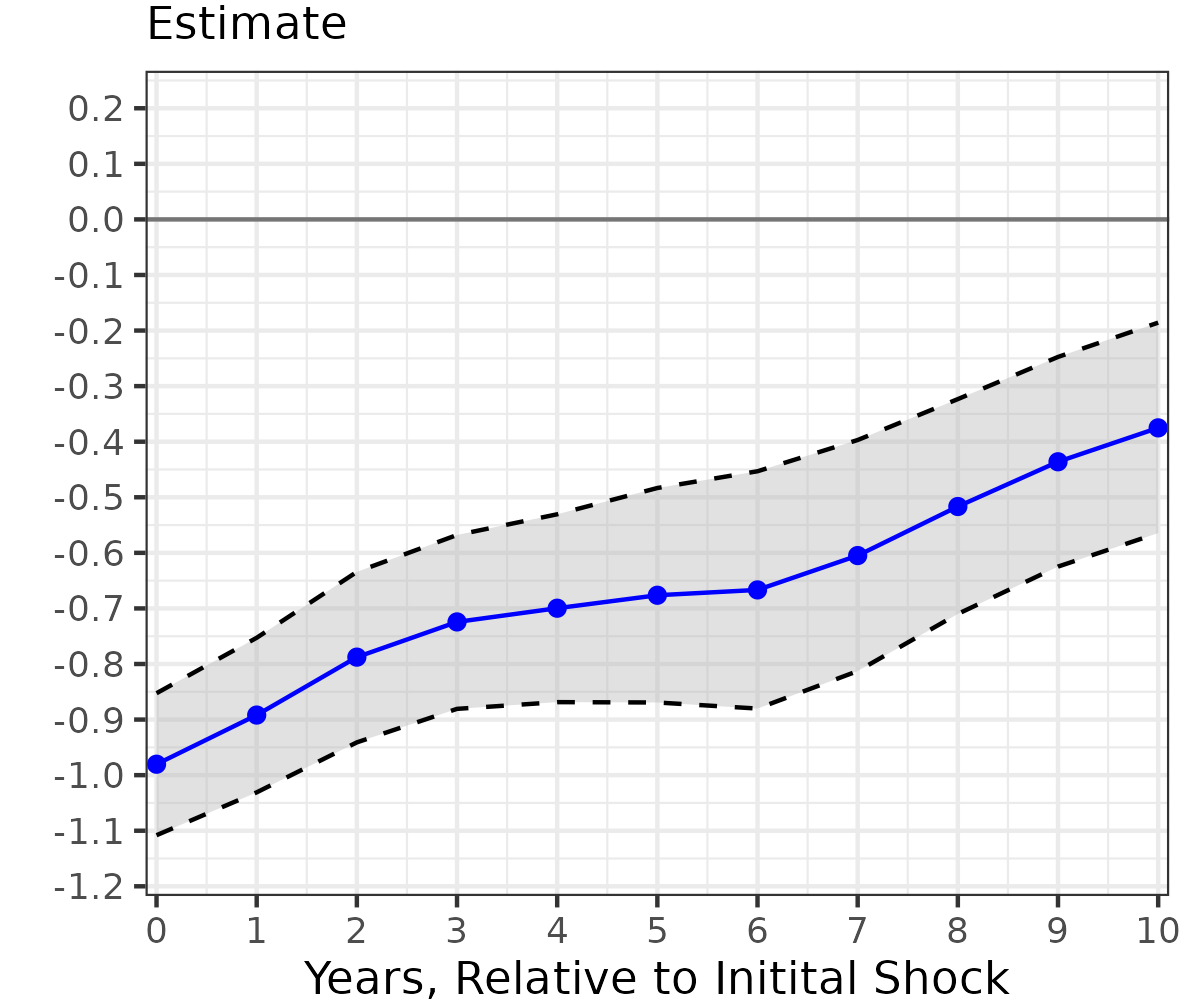
\includegraphics[width=0.6\textwidth]{figures/firststage-lp.png}
    \label{fig:firststage-lp}
    \justify
    \footnotesize
    \textbf{Note}:
    These figures show the local projections estimates of regression specification \eqref{eqn:firststage}, with the funding shift-share as an instrument for state funding, using IPEDS data.
    The coefficient estimate is effect of funding shift-share ($Z_{i,t}$) on state funding ($X_{i,t}$), while accounting for auto-correlation between different time periods --- i.e., between $Z_{i,t}, Z_{i,t-1}$ and $X_{i,t}, X_{i,t-1}$.
    These results use a $\log-\log$ specification, so the estimates are for the elasticity of state funding per student in a year $t+k$ with respect to funding shift-share in year $t$, where years $k = 0, \hdots, 10$ are on the $x$-axis. 
    Standard errors are clustered at the state-year level.
\end{figure}

\begin{table}[H]
    \singlespacing
    \centering
    \caption{Effect of State Funding on Areas of University Spending, IPEDS Data, IV Estimates.}
    \textbf{Panel A: units in \$ per student}
     
    \makebox[\textwidth][c]{\input{tables/expenditures-shock-rawcount.tex}}
    
    \textbf{Panel B: units in log \$ per student}
    
    \makebox[\textwidth][c]{
\begin{tabular}{@{\extracolsep{5pt}}lcccc} 
\\[-1.8ex]\hline 
\hline \\[-1.8ex] 
 & \multicolumn{4}{c}{Dependent Variable: Salary Expenditures} \\ 
\cline{2-5} 
\\[-1.8ex] & \multicolumn{2}{c}{Instruction} & \multicolumn{2}{c}{Research} \\ 
 & OLS & 2SLS & OLS & 2SLS \\ 
\\[-1.8ex] & (1) & (2) & (3) & (4)\\ 
\hline \\[-1.8ex] 
 State Funding & 0.089 & 0.076 & 0.032 & $-$0.036 \\ 
  & (0.045) & (0.065) & (0.045) & (0.142) \\ 
 \hline \\[-1.8ex] 
Observations & 14,242 & 14,242 & 14,242 & 14,242 \\ 
R$^{2}$ & 0.951 & 0.951 & 0.908 & 0.908 \\ 
\hline 
\hline \\[-1.8ex] 
\end{tabular} 
}
    
    \label{tab:expenditures-shock-reg}
    \justify
    \footnotesize
    \textbf{Note}:
    These tables show the IV estimates of regression specification \eqref{eqn:secondstage}, showing the effect of state funding (instrumented with the shift-share) on areas of university spending.
    Outcomes are measured in \$ student spending, so that the estimates representat the relationship between a \$1 increase in state funding on area of spending (or 1\% increase).    
    The ``outcome mean'' rows are spending in thousands \$ per student.
\end{table}

\newpage
\subsection{Illinois IBHED First Stage}
\label{sec:iv-model-indiv}

This paper uses data on individual professors in the Illinois university system, to investigate the effects of changes in university revenues on the individual professors at the universities.
The outcomes here now refer to individual professors (e.g., their salary and promotion rate), so requires adjustment to the empirical approach, leveraging variation in university funding for the years after a professor joins the university.

\autoref{eqn:rolling-instrument} defines a rolling-share variant of the instrument, $\tilde Z_{i(j),t}$, where the university's state funding share exposure is based in the year a professor joins the university --- and not the base period 1990--1993.
$j$ indexes each professor in year $t$, $\tau(j)$ for the year the professor first joins their institution.
Identifying $\tau(j)$ is possible for $j$ by restricting to all professors hired 2011-2021 --- i.e., in the years after the start of the full panel.
It is not possible to discern the hiring year for professors who  were hired in the years preceding 2011, and so the entire sample is only possible to analyse using the base-share in years 1990-1993 formulation.

\begin{align}
    \label{eqn:rolling-instrument}
    \tilde Z_{i(j),t} &\coloneqq - \left[
    \left( \frac{\text{Total State Funding}_{s(j),t}}{\text{Student Population}_{s(j),t}} \right)
    \left( \frac{\text{State Funding}_{\tau(j)}}{\text{Total Revenues}_{i,\tau(j)}} \right) \right]
\end{align}

This approach leverages an insight, made available by level of the data: that an individual professor is affected by changes in university revenues after they have joined the university.
\autoref{sec:iv-model-uni} considers the number of professors employed by the university; whether a professor becomes employed at the university is likely affected by that university's finances.
The formulation here takes as given that the professor is already employed at the university, and then projects the effect of changes in state funding on these \textit{incumbent} professors following the state funding shift-share.
\autoref{tab:firststage-illinois} presents the first-stage results in Illinois data.

\begin{table}[h!]
    \singlespacing
    \centering
    \caption{First Stage Estimates, for State Funding by Funding Shift-Share in IBHED Data.}
    \textbf{Panel A: units in \$ per student}
    
    \makebox[\textwidth][c]{
\begin{tabular}{@{\extracolsep{5pt}}lcccc} 
\\[-1.8ex]\hline 
\hline \\[-1.8ex] 
 & \multicolumn{4}{c}{Dependent Variable: State Funding} \\ 
\cline{2-5} 
\\[-1.8ex] & (1) & (2) & (3) & (4)\\ 
\hline \\[-1.8ex] 
 Funding Shock & $-$1.176 & $-$0.160 & $-$1.100 & $-$1.071 \\ 
  & (0.226) & (0.265) & (0.242) & (0.264) \\ 
  Tuition Revenue &  &  & $-$0.295 & 1.012 \\ 
  &  &  & (0.136) & (0.329) \\ 
  Constant &  & 9,716.437 &  & $-$1,708.334 \\ 
  &  & (1,805.394) &  & (2,716.150) \\ 
 \hline \\[-1.8ex] 
Uni. + Year fixed effects? & Yes & No & Yes & No \\ 
F stat. & 20.712 & 16.512 & 26.999 & 0.365 \\ 
Observations & 17,012 & 17,012 & 17,012 & 17,012 \\ 
R$^{2}$ & 0.918 & 0.0004 & 0.919 & 0.074 \\ 
\hline 
\hline \\[-1.8ex] 
\end{tabular} 
}
    
    \textbf{Panel B: units in log \$ per student}
    
    \makebox[\textwidth][c]{
\begin{tabular}{@{\extracolsep{5pt}}lcccc} 
\\[-1.8ex]\hline 
\hline \\[-1.8ex] 
 & \multicolumn{4}{c}{Dependent Variable: State Funding} \\ 
\cline{2-5} 
\\[-1.8ex] & (1) & (2) & (3) & (4)\\ 
\hline \\[-1.8ex] 
  State Funding & $-$1.000 & $-$0.877 & $-$0.987 & $-$0.726 \\ 
  & (0.018) & (0.046) & (0.026) & (0.155) \\ 
  Tuition Revenue & 0.538 & 0.536 &  &  \\ 
  & (0.334) & (0.270) &  &  \\ 
  Constant &  & $-$3.298 &  & 3.004 \\ 
  &  & (2.477) &  & (1.259) \\ 
 \hline \\[-1.8ex] 
Fixed effects? & Yes & No & Yes & No \\ 
F stat. & 3118.566 & 364.133 & 1394.217 & 21.88 \\ 
Observations & 70,743 & 187,634 & 70,743 & 187,634 \\ 
R$^{2}$ & 0.928 & 0.521 & 0.924 & 0.414 \\ 
\hline 
\hline \\[-1.8ex] 
\end{tabular} 
}
    
    \label{tab:firststage-illinois}
    \justify
    \footnotesize
    \textbf{Note}:
    These tables show the first stage OLS estimates of regression specification \eqref{eqn:secondstage1_indiv}, showing the effect of the funding shift-share on state funding to gauge performance as an instrument.
    Each observation is a professor-year, in the IBHED data, and funding data are merged from IPEDS.
    %Panel A shows the effect of an funding shift-share of \$-1 per student in the state on the number of \$'s of state funding per student at the university --- i.e.,
    %\$-1 funding shift-share per student in the state leads to \$1.176 less state funding per student at the university according to preferred specification column 1.
    Panel A shows the effect of a $-10$\% change funding shift-share per student in the state on $10$\% change in state funding per student at the university --- i.e.,
    $-10$\% funding shift-share per student in the state leads to $-9.77$\% less state funding per student at the university according to prefferred specification column 1.        
    Standard errors are clustered at the institution-year level, and institution $+$ year fixed effects are included where noted.
\end{table}

Exogeneity and relevance of the rolling-share instrument, $\tilde Z_{i(j),t}$, follows the same reasoning as that for the base-share instrument, $Z_{i,t}$, discussed in \autoref{sec:approp-shocks}.
The base-share instrument is appropriate for some outcomes with the individual Illinois professors, where appropriate.
We satisfy the assumptions for exogeneity by noting that none of the Illinois public campuses take the majority of state funding, and that the identification strategy relies on exogeneity in changes in state funding to individual professor-outcomes, following the year they joined the university.
Additionally, within-institution changes resulting from share reliance on state funding may be correlated with unobserved changes in the outcomes, so that \cite{NBERw27885} note the importance of controlling for the base share and state student population.
The formulation here implicitly controls for these factors via the fixed effects; results are relatively similar while including these controls with and without including fixed effects, and so are omitted.

The instrumental variables model is then defined as follows, where $i(j)$ refers to the institution that professor $j$ is employed at, and $Y_{j,t}$ for salary, rate of promotion, and propensity to leave the Illinois public university system.
The system includes fixed effects for the institution and first year of employment.
The instrument varies by institution, based in the year of first employment, so that these are the corresponding fixed effects and level of clustered standard errors.
\begin{eqnarray}
    \label{eqn:secondstage1_indiv}
    X_{i(j),t} &=& \theta_{i(j)} + \phi_{\tau(j)} + \delta \tilde Z_{i(j),t} + \epsilon_{i(j),t} \\
    \label{eqn:secondstage2_indiv}
    Y_{j,t} &=& \mu_{i(j)} + \nu_{\tau(j)} + \beta \widehat X_{i(j),t} + \varepsilon_{j,t}
\end{eqnarray}
We then interpret parameter $\beta$ as the effect of changes in state funding at an Illinois public university, via state funding shift-shares, on an individual professor's outcome $Y_{j,t}$.

\newpage
\begin{figure}[H]
    \centering
    \singlespacing
    \caption{Local Projection Estimates for Effect of State Funding on Faculty Promotion Rate at Illinois Public Universities, by Professor Group.}
    \begin{subfigure}[b]{0.495\textwidth}
        \centering
        \caption{First-stage Estimate.}
        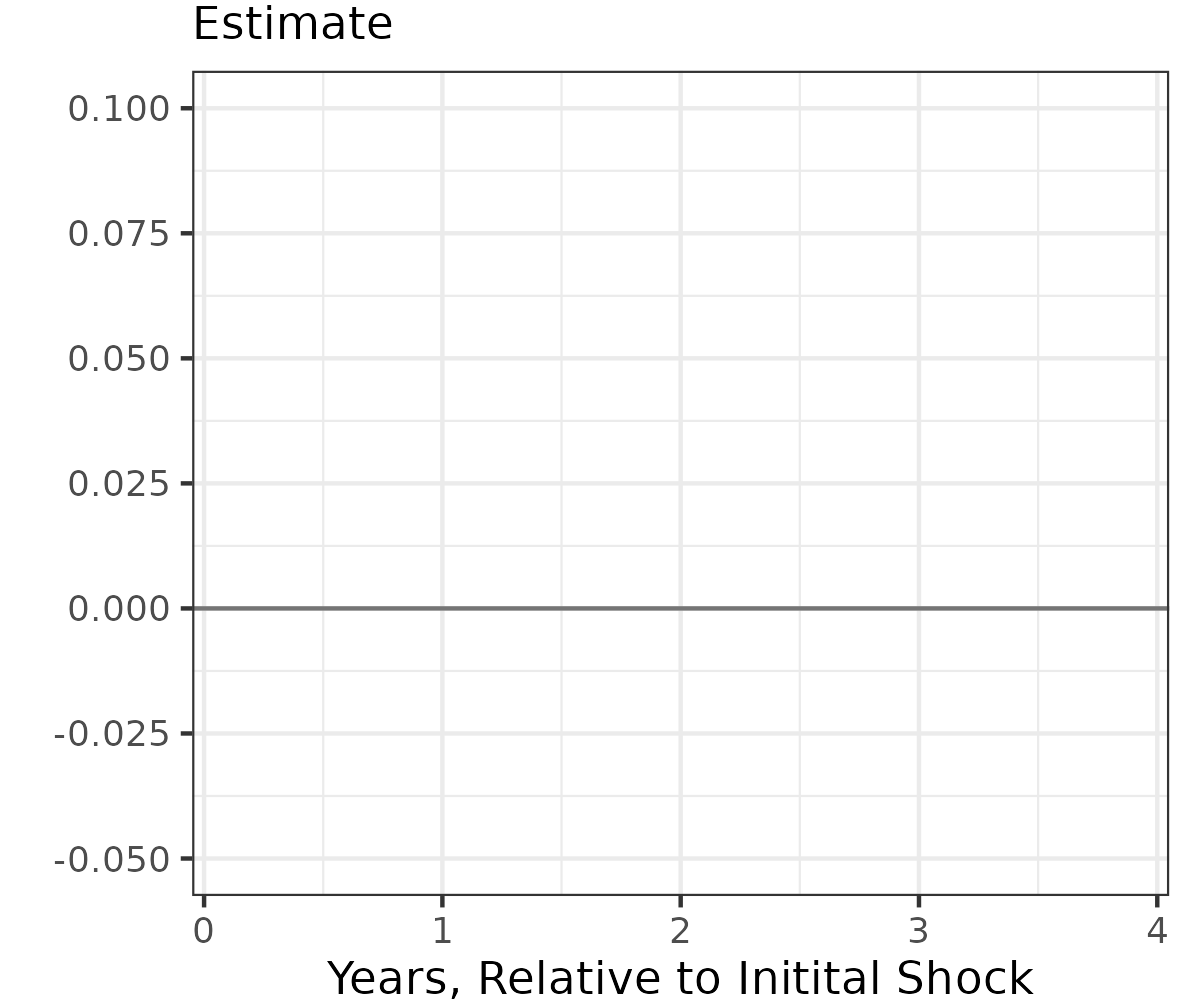
\includegraphics[width=\textwidth]{figures/firststage-illinois-lp-rolling.png}
        \label{fig:firststage-illinois-lp-rolling}
    \end{subfigure}
    \begin{subfigure}[b]{0.495\textwidth}
        \centering
        \caption{Lecturers.}
        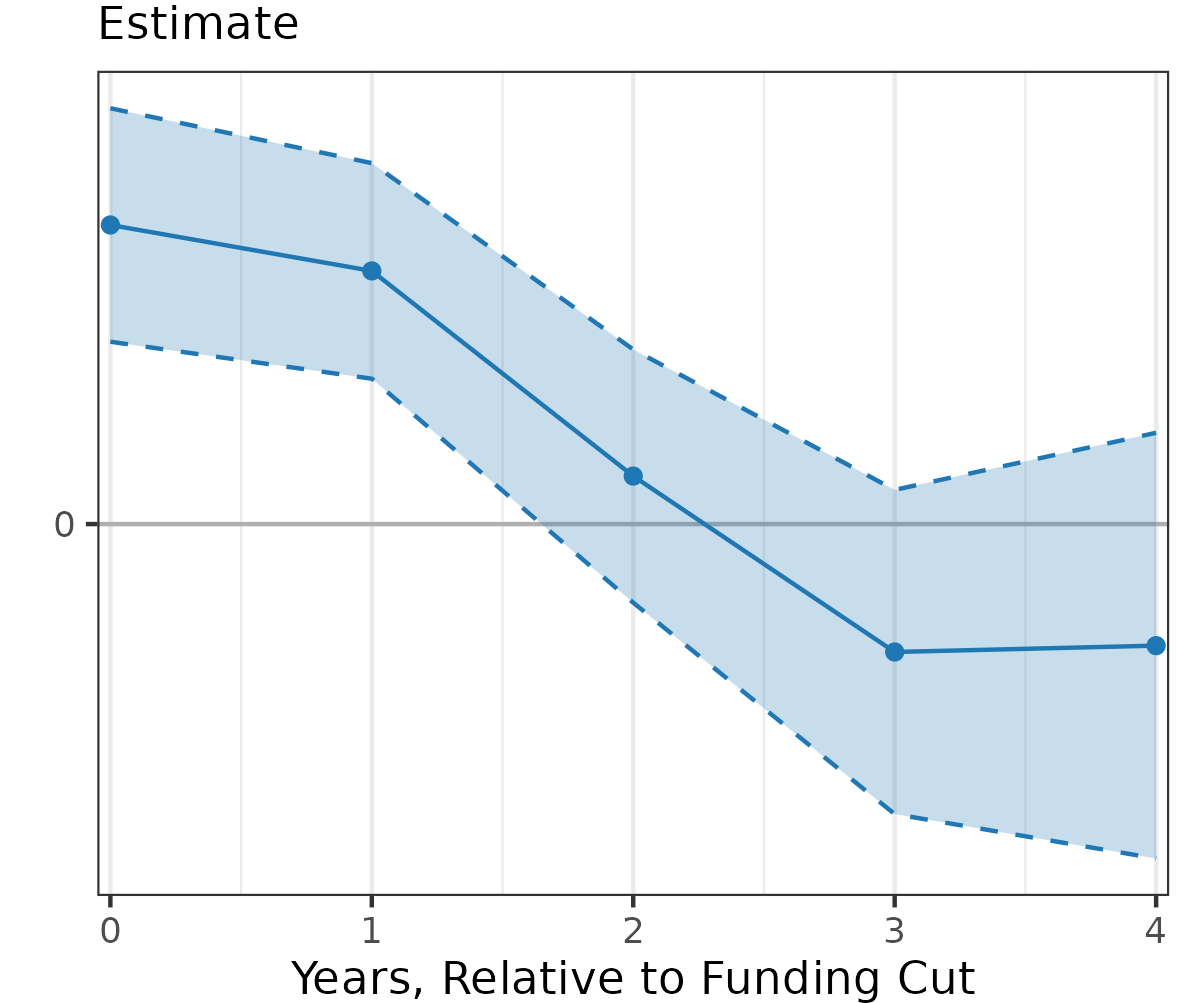
\includegraphics[width=\textwidth]{figures/promoted-lecturer-illinois-lp-rolling.png}
        \label{fig:promoted-lecturer-illinois-lp-rolling}
    \end{subfigure}
    \begin{subfigure}[b]{0.495\textwidth}
        \centering
        \caption{Assistant Professors.}
        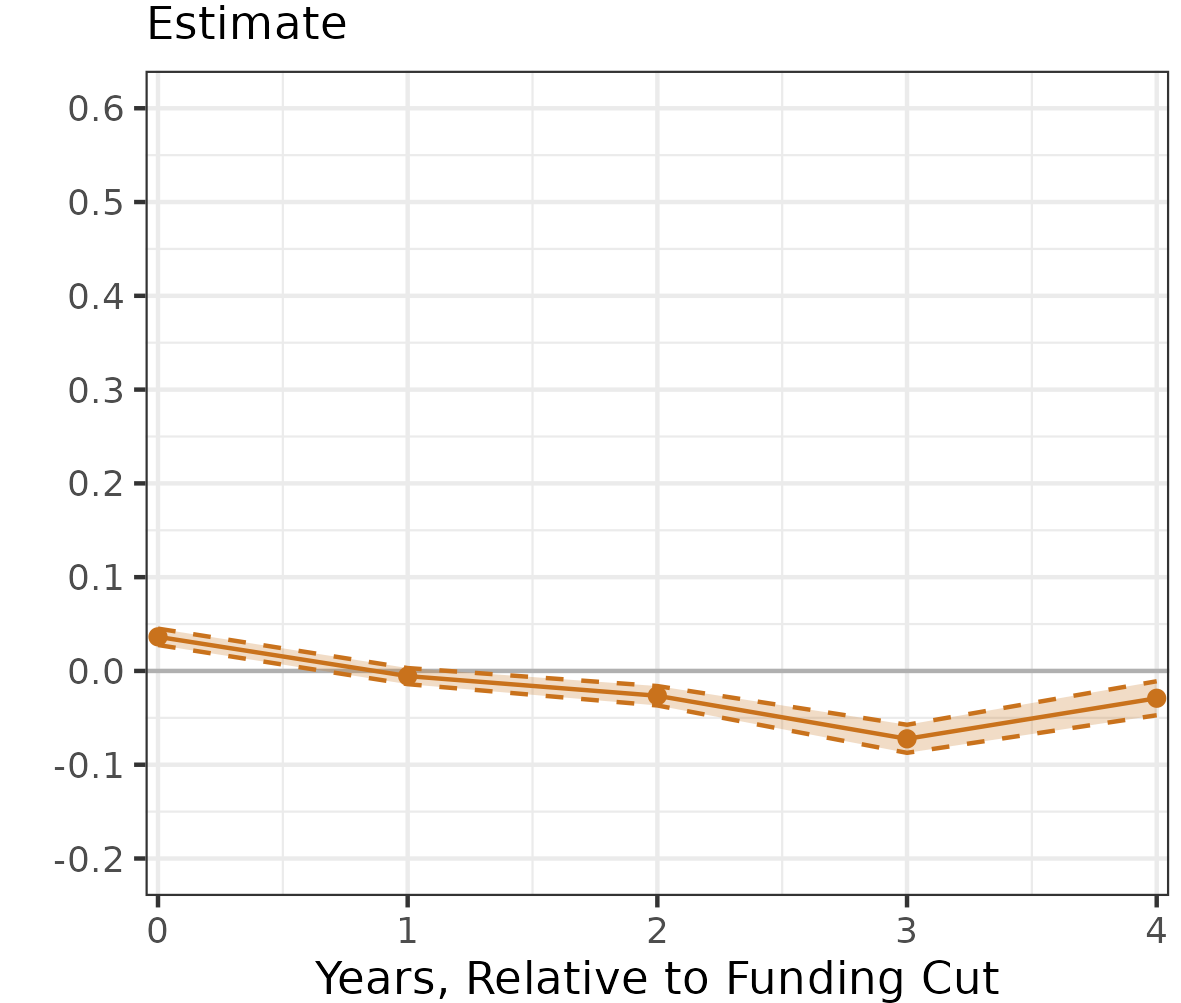
\includegraphics[width=\textwidth]{figures/promoted-assistant-illinois-lp-rolling.png}
        \label{fig:promoted-assistant-illinois-lp-rolling}
    \end{subfigure}
    \begin{subfigure}[b]{0.495\textwidth}
        \centering
        \caption{Full Professors.}
        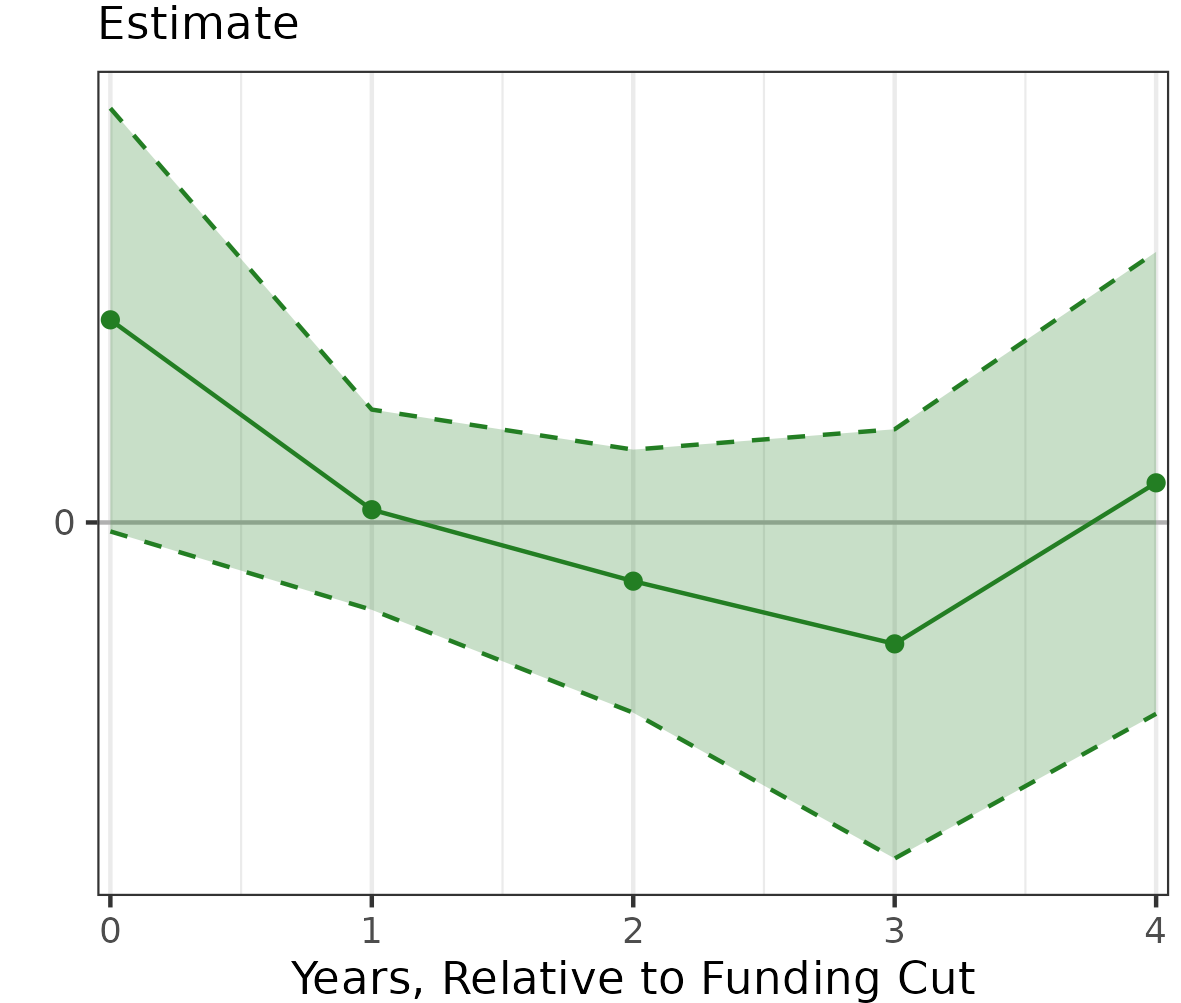
\includegraphics[width=\textwidth]{figures/promoted-full-illinois-lp-rolling.png}
        \label{fig:promoted-full-illinois-lp-rolling}
    \end{subfigure}
    \label{fig:promoted-illinois-lp-rolling}
    \justify
    \footnotesize
    \textbf{Note}:
    These figures show the local projections estimates of regression specification \eqref{eqn:secondstage}, with the funding shift-share as an instrument for state funding.
    The unit of analysis is an individual faculty member (at an Illinois public university); funding data come from IPEDS, and faculty promotion rate from IBHED.
    The coefficient estimate is effect of state funding ($X_{i(j),t}$) on faculty promotion rate ($Y_{j,t}$), using the funding shift-share instrument ($Z_{i(j),t}$), while accounting for auto-correlation between different time periods --- i.e., between $X_{i(j),t}, X_{i(j),t-1}$ and $Y_{i(j),t}, Y_{i(j),t-1}$.
    These results use a $\log-\log$ specification, so the estimates are for the rate of promotion in a year $t+k$ affected by a 1\% change in state funding in year $t$, where years $k = 0, \hdots, 4$ are on the $x$-axis. 
    Standard errors are clustered at the university-year level, and \autoref{sec:iv-model-indiv} fully describes the differences in empirical specification when unit of analysis is an individual faculty member.
\end{figure}

\newpage
\begin{table}[H]
    \singlespacing
    \centering
    \caption{Effects of Changes in State Funding on University Faculty Composition, in Illinois 2010--2021, OLS and 2SLS Estimates.}

    \textbf{Panel A: units in \$ per student}

    \makebox[\textwidth][c]{
\begin{tabular}{@{\extracolsep{5pt}}lcccccccc} 
\\[-1.8ex]\hline 
\hline \\[-1.8ex] 
 & \multicolumn{8}{c}{Dependent Variable: Employment Count by Professor Group} \\ 
\cline{2-9} 
\\[-1.8ex] & \multicolumn{2}{c}{Lecturer} & \multicolumn{2}{c}{Assistant} & \multicolumn{2}{c}{Full} & \multicolumn{2}{c}{All} \\ 
 & OLS & 2SLS & OLS & 2SLS & OLS & 2SLS & OLS & 2SLS \\ 
\\[-1.8ex] & (1) & (2) & (3) & (4) & (5) & (6) & (7) & (8)\\ 
\hline \\[-1.8ex] 
 State Funding & $-$3.729 & 0.376 & 0.415 & 3.208 & $-$1.269 & 0.117 & $-$4.084 & 3.890 \\ 
  & (1.721) & (1.725) & (1.728) & (2.493) & (1.548) & (1.200) & (4.352) & (5.668) \\ 
 \hline \\[-1.8ex] 
Outcome Mean & 351.306 & 351.306 & 273.757 & 273.757 & 477.597 & 477.597 & 1303.014 & 1303.014 \\ 
Observations & 144 & 144 & 144 & 144 & 144 & 144 & 144 & 144 \\ 
R$^{2}$ & 0.886 & 0.882 & 0.970 & 0.969 & 0.991 & 0.991 & 0.981 & 0.980 \\ 
\hline 
\hline \\[-1.8ex] 
\end{tabular} 
}
    
    \textbf{Panel B: units in log \$ per student}
    
    \makebox[\textwidth][c]{
\begin{tabular}{@{\extracolsep{5pt}}lcccccccc} 
\\[-1.8ex]\hline 
\hline \\[-1.8ex] 
 & \multicolumn{8}{c}{Dependent Variable: Employment Count by Professor Group} \\ 
\cline{2-9} 
\\[-1.8ex] & \multicolumn{2}{c}{Lecturer} & \multicolumn{2}{c}{Assistant} & \multicolumn{2}{c}{Full} & \multicolumn{2}{c}{All} \\ 
 & OLS & 2SLS & OLS & 2SLS & OLS & 2SLS & OLS & 2SLS \\ 
\\[-1.8ex] & (1) & (2) & (3) & (4) & (5) & (6) & (7) & (8)\\ 
\hline \\[-1.8ex] 
 State Funding & $-$0.015 & $-$0.017 & 0.049 & 0.058 & 0.007 & $-$0.029 & 0.004 & $-$0.008 \\ 
  & (0.033) & (0.026) & (0.045) & (0.038) & (0.021) & (0.032) & (0.028) & (0.022) \\ 
 \hline \\[-1.8ex] 
Outcome Mean & 2.523 & 2.523 & 1.491 & 1.491 & 2.729 & 2.729 & 8.141 & 8.141 \\ 
Observations & 144 & 144 & 144 & 144 & 144 & 144 & 144 & 144 \\ 
R$^{2}$ & 0.700 & 0.700 & 0.789 & 0.789 & 0.839 & 0.836 & 0.633 & 0.632 \\ 
\hline 
\hline \\[-1.8ex] 
\end{tabular} 
}

    \label{tab:facultycount-illinois-reg}
    \justify
    \footnotesize
    \textbf{Note}:
    These tables show the second stage OLS and 2SLS estimates of regression specification \eqref{eqn:secondstage}, showing the effect of state funding changes on number of faculty per student in Illinois universities, using the funding shift-share to instrument for state funding in the columns labelled 2SLS.
    Each observation is a public university-year in the state of Illinois, where funding data come from IPEDS and faculty count come from IBHED data.
    Panel A shows the effect of a fall in state funding \$$-1,000$ per student in the state on the number of professors.
    Panel B shows the effect of a $10$\% change in state funding per student at the university on the 10\% change in the number of professors per students.
    Outcome-mean is the mean of the outcome, for Panel A the number of professors per student, for Panel B the number of faculty per student.
    Panel B uses $\log$ faculty count per student as the outcome, though the outcome mean is count of faculty per student (not in $\log$ terms).
    Standard errors are clustered at the university-year level, and university $+$ year fixed effects are included through--out.
\end{table}

\newpage
\begin{figure}[H]
    \centering
    \singlespacing
    \caption{Local Projection Estimates for Effect of State Funding on Faculty Exit Rate at Illinois Public Universities, by Professor Group.}
    \begin{subfigure}[b]{0.495\textwidth}
        \centering
        \caption{Lecturers.}
        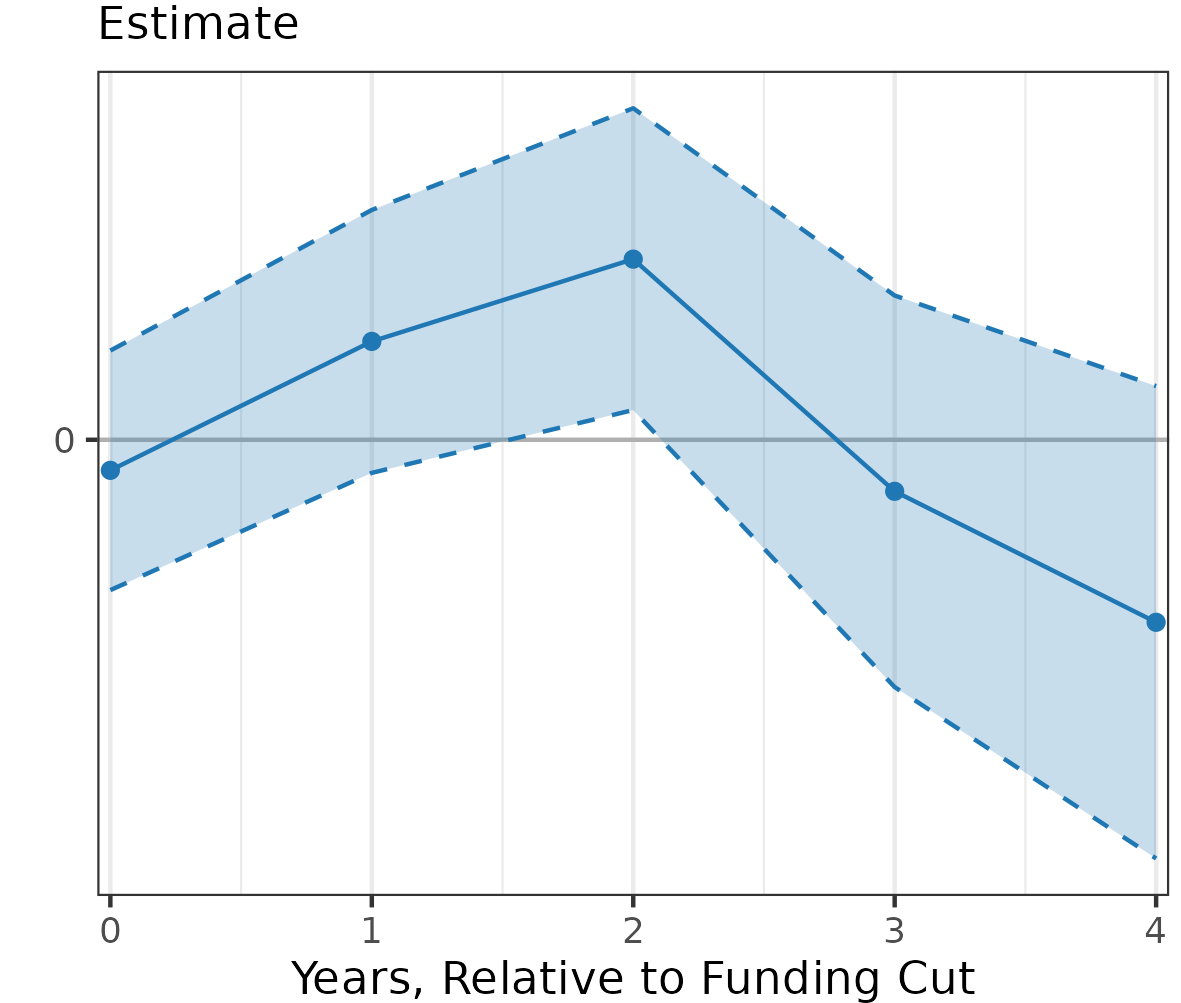
\includegraphics[width=\textwidth]{figures/exit-lecturer-illinois-lp-rolling.png}
        \label{fig:exit-lecturer-illinois-lp-rolling}
    \end{subfigure}
    \begin{subfigure}[b]{0.495\textwidth}
        \centering
        \caption{Assistant Professors.}
        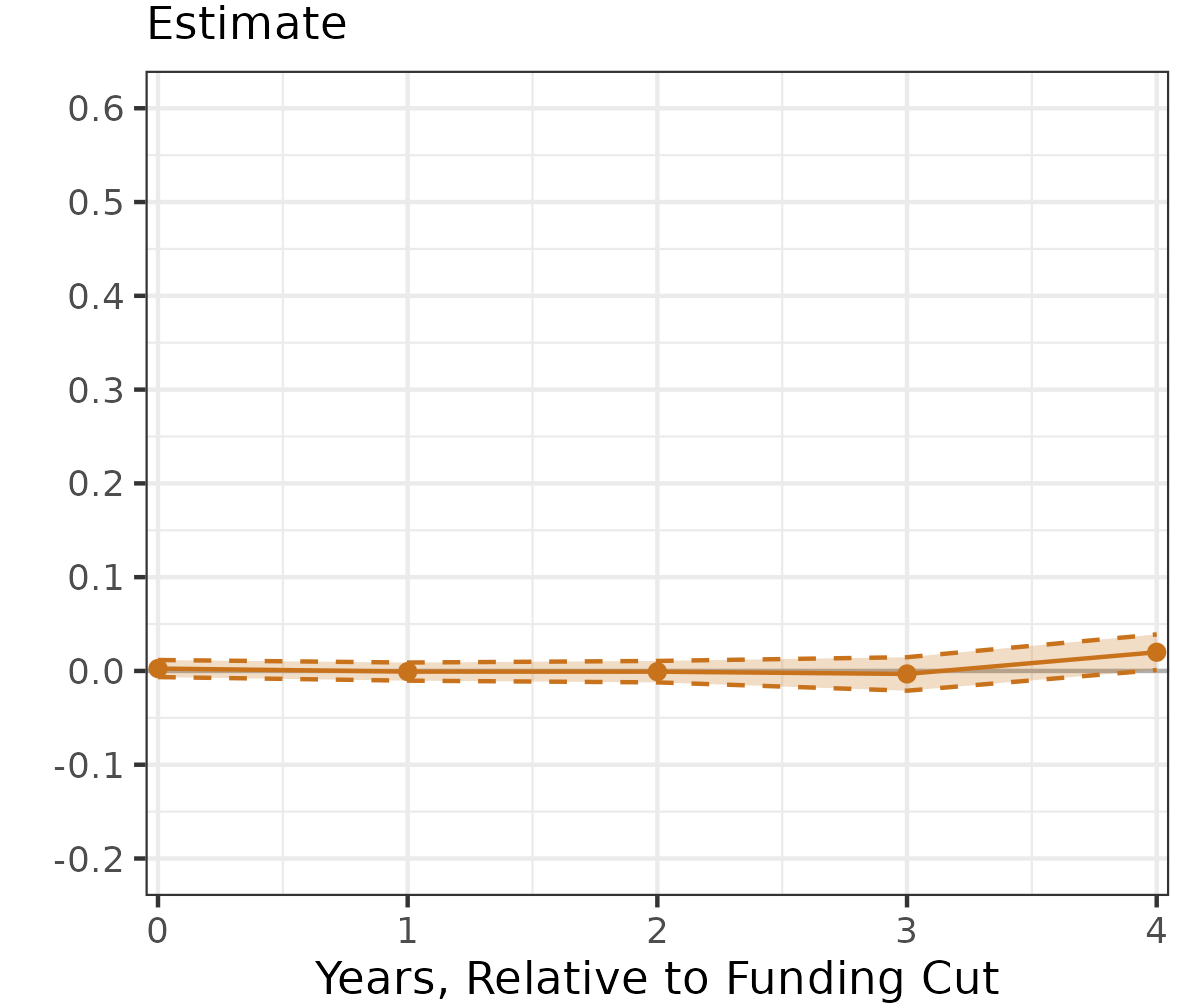
\includegraphics[width=\textwidth]{figures/exit-assistant-illinois-lp-rolling.png}
        \label{fig:exit-assistant-illinois-lp-rolling}
    \end{subfigure}
    \begin{subfigure}[b]{0.495\textwidth}
        \centering
        \caption{Full Professors.}
        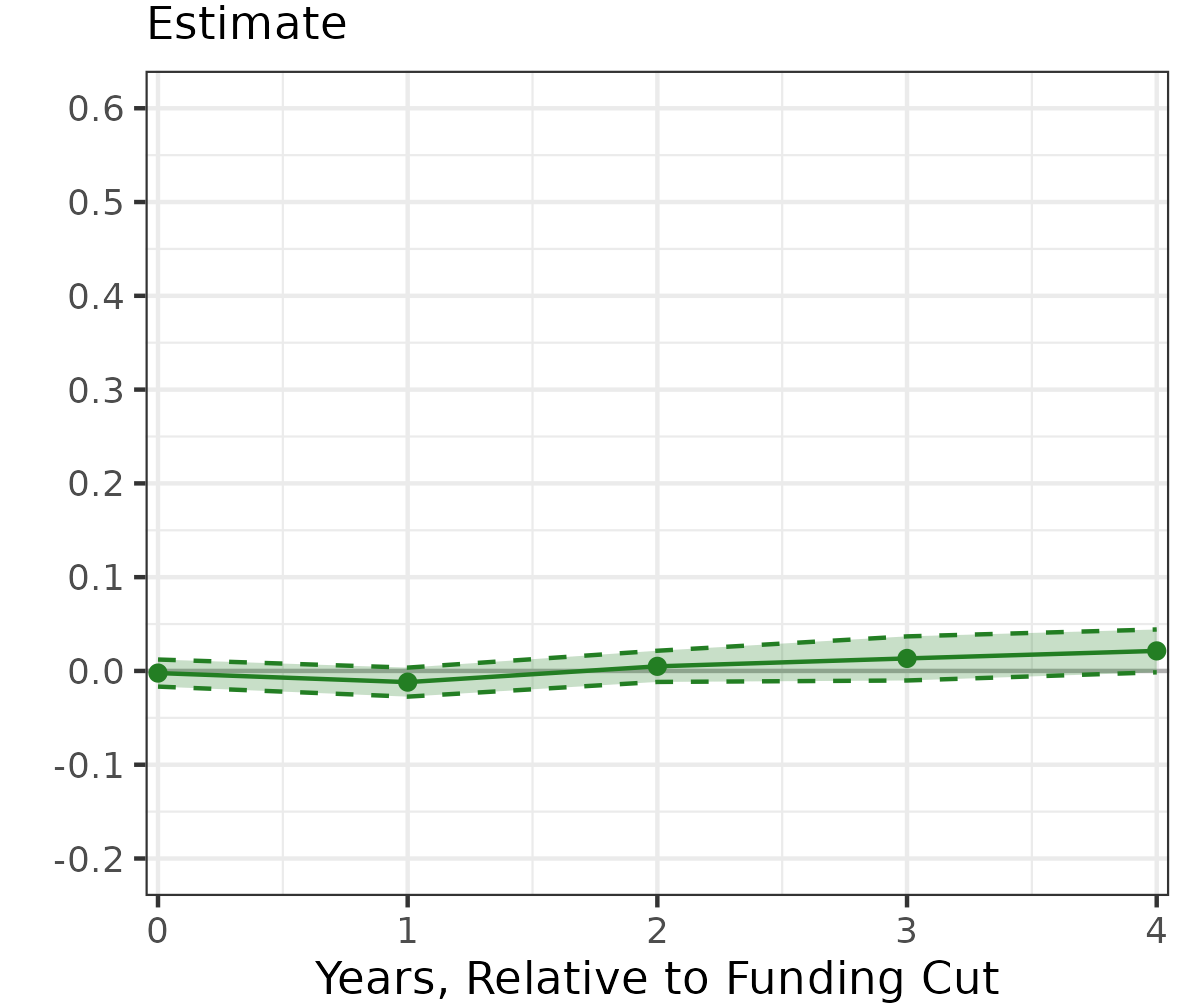
\includegraphics[width=\textwidth]{figures/exit-full-illinois-lp-rolling.png}
        \label{fig:exit-full-illinois-lp-rolling}
    \end{subfigure}
    \begin{subfigure}[b]{0.495\textwidth}
        \centering
        \caption{Administrator Professors.}
        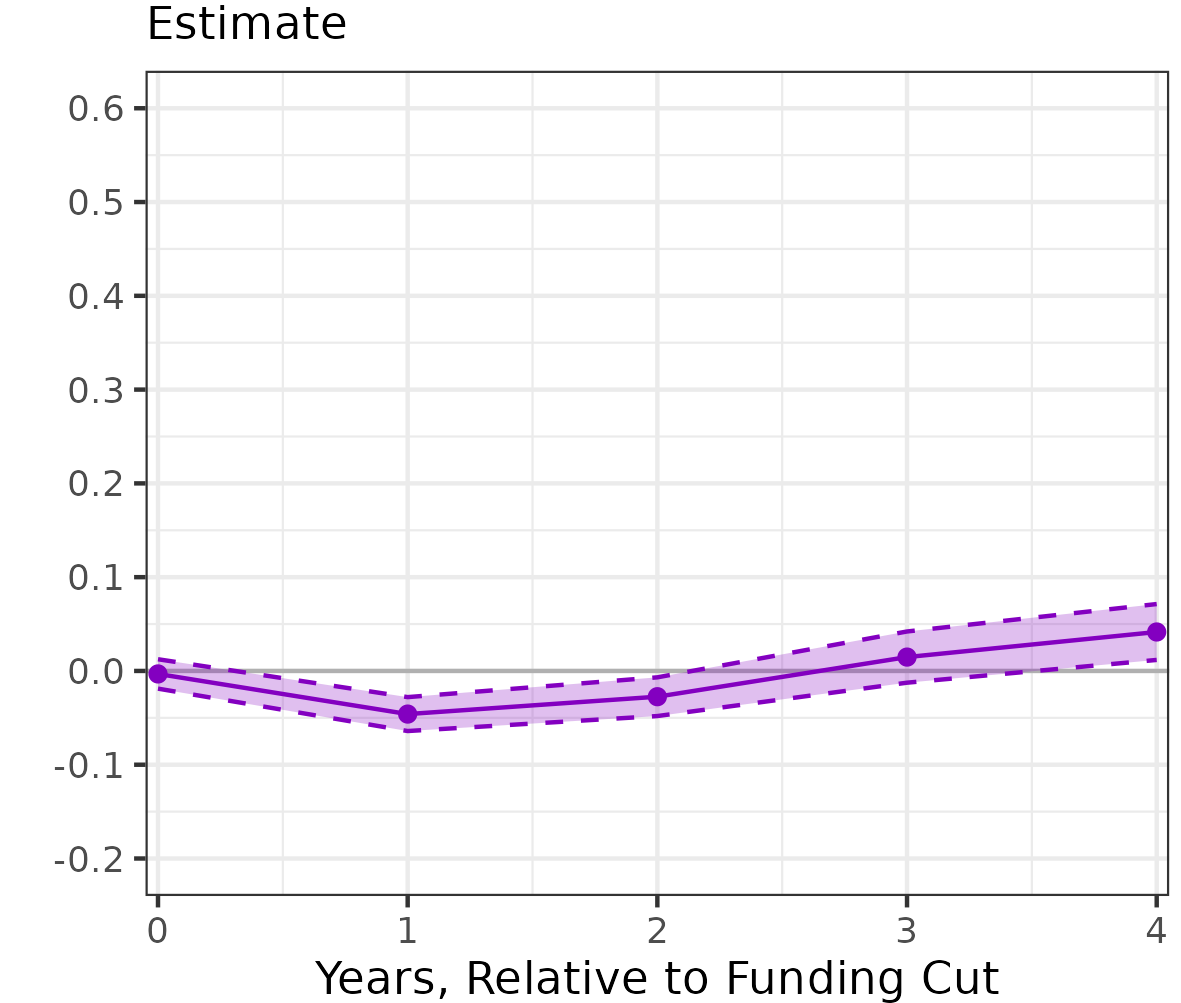
\includegraphics[width=\textwidth]{figures/exit-administrator-illinois-lp-rolling.png}
        \label{fig:exit-administrator-illinois-lp-rolling}
    \end{subfigure}
    \label{fig:exit-illinois-lp-rolling}
    \justify
    \footnotesize
    \textbf{Note}:
    These figures show the local projections estimates of regression specification \eqref{eqn:secondstage}, with the funding shift-share as an instrument for state funding.
    The unit of analysis is an individual faculty member (at an Illinois public university); funding data come from IPEDS, and faculty promotion rate from IBHED.
    The coefficient estimate is effect of state funding ($X_{i(j),t}$) on faculty promotion rate ($Y_{j,t}$), using the funding shift-share instrument ($Z_{i(j),t}$), while accounting for auto-correlation between different time periods --- i.e., between $X_{i(j),t}, X_{i(j),t-1}$ and $Y_{i(j),t}, Y_{i(j),t-1}$.
    These results use a rate$-\log$ specification, so the estimates are for the rate of promotion in a year $t+k$ affected by a 1\% change in state funding in year $t$, where years $k = 0, \hdots, 4$ are on the $x$-axis. 
    Standard errors are clustered at the university-year level, and \autoref{sec:iv-model-indiv} fully describes the differences in empirical specification when unit of analysis is an individual faculty member.
\end{figure}

\newpage
\subsection{Professor Hiring}
\label{sec:appendix-hiring}

These results were produced by integrating the total count of professor hires for 2010--2021 for the top-ranked 180 US universities with a sum of the funding variables, and then estimating the models specified in \autoref{sec:iv-model-uni}.
There were no observable differences in the hiring rate of male versus female faculty.

\begin{table}[H]
    \singlespacing
    \centering
    \caption{OLS and 2SLS Estimates for University Faculty Hires, in Illinois 2011--2021.}

    \textbf{Panel A: units in \$ per student}

    \makebox[\textwidth][c]{
\begin{tabular}{@{\extracolsep{5pt}}lcccccccc} 
\\[-1.8ex]\hline 
\hline \\[-1.8ex] 
 & \multicolumn{8}{c}{Dependent Variable: Yearly New Hires by Professor Group} \\ 
\cline{2-9} 
\\[-1.8ex] & \multicolumn{2}{c}{Lecturers} & \multicolumn{2}{c}{Asst. Professors} & \multicolumn{2}{c}{Full Professors} & \multicolumn{2}{c}{All Faculty} \\ 
 & OLS & 2SLS & OLS & 2SLS & OLS & 2SLS & OLS & 2SLS \\ 
\\[-1.8ex] & (1) & (2) & (3) & (4) & (5) & (6) & (7) & (8)\\ 
\hline \\[-1.8ex] 
 State Funding & $-$2.551 & $-$2.280 & 0.060 & $-$5.126 & $-$0.095 & $-$2.562 & $-$2.677 & 23.012 \\ 
  & (1.420) & (9.168) & (0.675) & (7.210) & (0.249) & (7.051) & (2.185) & (52.652) \\ 
 \hline \\[-1.8ex] 
Outcome Mean & 73.275 & 73.275 & 42.771 & 42.771 & 12.301 & 12.301 & 151.932 & 151.932 \\ 
Observations & 131 & 131 & 131 & 131 & 113 & 113 & 132 & 132 \\ 
R$^{2}$ & 0.839 & 0.839 & 0.934 & 0.902 & 0.788 & 0.752 & 0.918 & 0.793 \\ 
\hline 
\hline \\[-1.8ex] 
\end{tabular} 
}
    
    \textbf{Panel B: units in log \$ per student}
    
    \makebox[\textwidth][c]{
\begin{tabular}{@{\extracolsep{5pt}}lcccccccc} 
\\[-1.8ex]\hline 
\hline \\[-1.8ex] 
 & \multicolumn{8}{c}{Dependent Variable: Employment Count} \\ 
\cline{2-9} 
\\[-1.8ex] & \multicolumn{2}{c}{Lecturers} & \multicolumn{2}{c}{Asst. Professors} & \multicolumn{2}{c}{Full Professors} & \multicolumn{2}{c}{All Faculty} \\ 
 & OLS & 2SLS & OLS & 2SLS & OLS & 2SLS & OLS & 2SLS \\ 
\\[-1.8ex] & (1) & (2) & (3) & (4) & (5) & (6) & (7) & (8)\\ 
\hline \\[-1.8ex] 
 State Funding & 0.120 & 0.158 & 0.172 & 0.174 & 0.191 & 0.235 & 0.046 & 0.082 \\ 
  & (0.071) & (0.065) & (0.154) & (0.143) & (0.113) & (0.137) & (0.080) & (0.047) \\ 
 \hline \\[-1.8ex] 
Outcome Mean & 0.494 & 0.494 & 0.234 & 0.234 & 0.051 & 0.051 & 0.993 & 0.993 \\ 
Observations & 131 & 131 & 131 & 131 & 113 & 113 & 132 & 132 \\ 
R$^{2}$ & 0.749 & 0.749 & 0.482 & 0.482 & 0.628 & 0.627 & 0.580 & 0.579 \\ 
\hline 
\hline \\[-1.8ex] 
\end{tabular} 
}
    \label{tab:facultyhires-illinois-reg}
    \vspace{-0.5cm}
    \justify
    \footnotesize
    \textbf{Note}:
    These tables show the second stage OLS and 2SLS estimates of regression specification \eqref{eqn:secondstage}, showing the effect of state funding changes on number of faculty hires at Illinois universities, using the funding shift-share to instrument for state funding in the columns labelled 2SLS.
    Each observation is a public university-year in the state of Illinois, where funding data come from IPEDS and faculty count come from IBHED data.
    Panel A shows the effect of a fall in state funding \$$-1,000$ per student in the state on the number of new faculty hires by position.
    Panel B shows the effect of a $10$\% change in state funding per student at the university on the 10\% change in the number of faculty hires per students.
    Outcome-mean is the mean of the outcome, for Panel A the number of faculty hires, for Panel B the number of faculty hires per student.
    Panel B uses new faculty hires per student as the outcome (in $\log$ terms), though the outcome mean is count of new faculty hires per student (not in $\log$ terms).
    Standard errors are clustered at the university-year level, and university $+$ year fixed effects are included through--out.
\end{table}

\vspace{-0.5cm}
\begin{figure}[H]
    \centering
    \singlespacing
    \caption{Correlation Between State Funding and Total Count Professors Hired, 2011--2021.}
    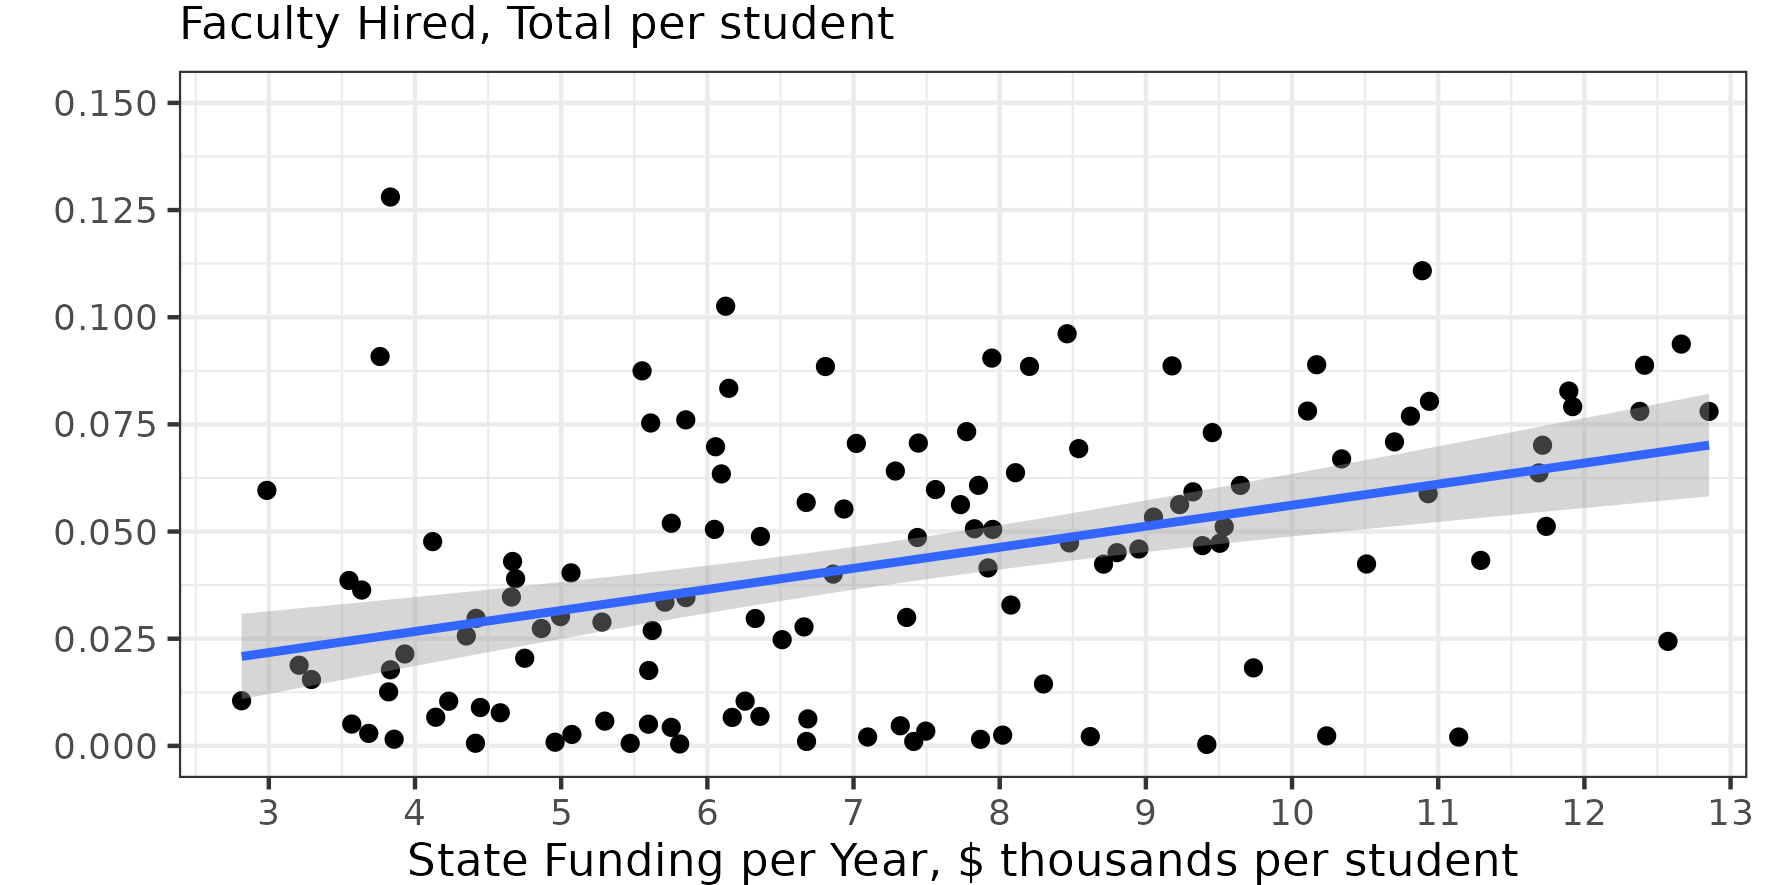
\includegraphics[width=0.75\textwidth]{figures/hiring-correlation.png}
    \label{fig:hiring-correlation}
    \justify
    \footnotesize
    \textbf{Note}:
    This figure shows the correlation between total state funding per student and total professors hired, 2010--2021.
    Funding data are taken from IPEDS, and data on professor hiring  from \cite{wapman2022quantifying,wapman2022zenodo}.
\end{figure}

\begin{table}[h!]
    \singlespacing
    \centering
    \caption{OLS and 2SLS Estimates for Professor Hiring, Total for 2011--2020.}
    \makebox[\textwidth][c]{
\begin{tabular}{@{\extracolsep{5pt}}lcccccc} 
\\[-1.8ex]\hline 
\hline \\[-1.8ex] 
 & \multicolumn{6}{c}{Dependent Variable: Professor Hiring Count} \\ 
\cline{2-7} 
\\[-1.8ex] & \multicolumn{2}{c}{Men} & \multicolumn{2}{c}{Women} & \multicolumn{2}{c}{Total} \\ 
 & OLS & 2SLS & OLS & 2SLS & OLS & 2SLS \\ 
\\[-1.8ex] & (1) & (2) & (3) & (4) & (5) & (6)\\ 
\hline \\[-1.8ex] 
 State Funding & 0.805 & 1.308 & 0.845 & 1.325 & 0.848 & 1.306 \\ 
  & (0.222) & (0.365) & (0.235) & (0.335) & (0.220) & (0.352) \\ 
 \hline \\[-1.8ex] 
Observations & 157 & 157 & 157 & 157 & 157 & 157 \\ 
R$^{2}$ & 0.396 & 0.366 & 0.415 & 0.383 & 0.408 & 0.381 \\ 
\hline 
\hline \\[-1.8ex] 
\end{tabular} 
}
    \label{tab:hiring-shock-reg}
    \justify
    \footnotesize
    \textbf{Note}: 
    This table show the second stage 2SLS estimates of regression specification \eqref{eqn:secondstage}, showing the effect of state funding changes on the number of faculty hires (per student) total for 2011--2021 at US public universities, using the funding shift-share to instrument for state funding.
    Yearly variation in total hires is not observed here, so only the total hires across 2011--2021 for 157 universities, can be considered.
    Each observation is a public university across the years 2011--2021, where data on total funding across 2011--2021 come from IPEDS and faculty count total from \citep{wapman2022quantifying,wapman2022zenodo}.
    The panels show the effect of a $1$\% change in state funding per student at the university (total for 2011--2021) on the number of new faculty hires by gender (and all).
    Standard errors are clustered at the state level, and state fixed effects are included through--out.
\end{table}

\newpage
\subsection{Robustness Checks}

\begin{table}[H]
    \singlespacing
    \centering
    \caption{Effects of State Funding on Faculty Counts, IPEDS 1990--2021, IV Estimates by Institution Selectivity.}

    \textbf{Panel A: units in \$ per student}

    \makebox[\textwidth][c]{
        \begin{tabular}{@{\extracolsep{5pt}}lcccccl} 
            \\[-1.8ex]\hline 
            \hline \\[-1.8ex]
            & First-stage & Lecturers & Asst. Professors & Full Professors & All Faculty & Observations \\ 
            \cline{2-7} 
            \\[-1.8ex]
            % latex table generated in R 4.3.1 by xtable 1.8-4 package
% Tue Apr 30 17:23:04 2024
  &  &  &  &  &  &  \\ 
  Most Selective: & -1.804 & 0.176 & 5.421 & 3.011 & 14.298 & 367 \\ 
   & (0.178) & (1.836) & (2.389) & (4.015) & (10.112) &  \\ 
   & [13036.59] & [0.004] & [0.011] & [0.033] & [0.05] &  \\ 
  Selective: & -5.555 & -0.089 & 0.025 & 0.044 & 0.022 & 815 \\ 
   & (0.324) & (0.019) & (0.006) & (0.004) & (0.003) &  \\ 
   & [12084.012] & [0.005] & [0.011] & [0.03] & [0.046] &  \\ 
  Unranked: & -7.264 & -0.058 & 0.018 & 0.017 & 0.008 & 15830 \\ 
   & (0.272) & (0.005) & (0.002) & (0.002) & (0.001) &  \\ 
   & [10206.27] & [0.006] & [0.012] & [0.022] & [0.041] &  \\ 
  
            \\[-1.8ex] \hline 
            \hline 
        \end{tabular}}
    
        \vspace{0.2cm}
    \textbf{Panel B: units in log \$ per student}
    
    \makebox[\textwidth][c]{
        \begin{tabular}{@{\extracolsep{5pt}}lcccccl} 
            \\[-1.8ex]\hline 
            \hline \\[-1.8ex]
            & First-stage & Lecturers & Asst. Professors & Full Professors & All Faculty & Observations \\ 
            \cline{2-7} 
            \\[-1.8ex]
            % latex table generated in R 4.3.1 by xtable 1.8-4 package
% Tue Apr 30 17:23:04 2024
  &  &  &  &  &  &  \\ 
  Most Selective: & -0.944 & -0.201 & 0.162 & 0.001 & -0.01 & 367 \\ 
   & (0.043) & (0.134) & (0.069) & (0.041) & (0.037) &  \\ 
   & [13036.59] & [0.004] & [0.011] & [0.033] & [0.05] &  \\ 
  Selective: & -1.067 & -0.465 & 0.129 & 0.229 & 0.116 & 815 \\ 
   & (0.022) & (0.092) & (0.031) & (0.018) & (0.016) &  \\ 
   & [12084.012] & [0.005] & [0.011] & [0.03] & [0.046] &  \\ 
  Unranked: & -0.965 & -0.436 & 0.137 & 0.131 & 0.062 & 15830 \\ 
   & (0.019) & (0.032) & (0.015) & (0.012) & (0.009) &  \\ 
   & [10206.27] & [0.006] & [0.012] & [0.022] & [0.041] &  \\ 
  
            \\[-1.8ex] \hline 
            \hline 
        \end{tabular}}
    \label{tab:facultycount-heterogeneity}
    \justify
    \footnotesize
    \textbf{Note}:
    These tables show the IV estimates of regression specification \eqref{eqn:secondstage}, 
    in the same manner as \autoref{tab:facultycount-shock-reg}, but restricting to institutions ranked as most selective, selective, and unranked by \cite{barrons2009} --- and including state
    The first column presents the coefficient between state funding and shift-share IV, which is a string first-stage among every level of selectivity for public universities.
    The other columns show the coefficient between state funding the count of faculty per students.
    For example, Row 1 of panel B shows that a $10\%$ cut in the state shift-share leads to a fall of $9.44\%$ in state funding for the public universities ranked as ``most selective.''
    Standard errors for the coefficient estimates are in brackets, and the outcome mean are in square brackets beneath.
\end{table}

\begin{table}[H]
    \singlespacing
    \centering
    \caption{First-stage Robustness Checks for Effects of State Funding Shift-Share on State Funding, OLS Estimates.}
    \makebox[\textwidth][c]{
\begin{tabular}{@{\extracolsep{5pt}}lcc} 
\\[-1.8ex]\hline 
\hline \\[-1.8ex] 
 & \multicolumn{2}{c}{Dependent Variable: State Funding} \\ 
\cline{2-3} 
 & Raw Count Units & Log Units \\ 
\\[-1.8ex] & (1) & (2)\\ 
\hline \\[-1.8ex] 
 State Funding & $-$1.299 & $-$1.050 \\ 
  & (0.172) & (0.041) \\ 
  State Funding, Base Share \% & $-$95.489 & $-$0.895 \\ 
  & (40.941) & (0.141) \\ 
  Acceptance Rate, \% & $-$13.540 & $-$0.012 \\ 
  & (15.208) & (0.046) \\ 
  6--Year Completion Rate, \% & 69.341 & 0.148 \\ 
  & (23.718) & (0.074) \\ 
  Tuition Revenue, \$ millions & 1.223 & 0.350 \\ 
  & (1.433) & (0.040) \\ 
  Enrolment, FTE thousands & $-$4.748 & $-$0.669 \\ 
  & (58.129) & (0.055) \\ 
  State Enrolment, thousands & 2.215 & 0.258 \\ 
  & (1.236) & (0.053) \\ 
  Percent of State Enrolment & 0.803 & 0.0003 \\ 
  & (3.356) & (0.0001) \\ 
 \hline \\[-1.8ex] 
Units  & Raw counts & Log, \% terms \\ 
F stat. & 57.356 & 660.878 \\ 
State + Year fixed effects? & Yes & Yes \\ 
Observations & 13,687 & 13,687 \\ 
R$^{2}$ & 0.382 & 0.453 \\ 
\hline 
\hline \\[-1.8ex] 
\end{tabular} 
}
    \label{tab:firststage-robustness-checks}
    \justify
    \footnotesize
    \textbf{Note}:
    These tables show the second stage OLS and 2SLS estimates of regression specification \eqref{eqn:firststage}, showing the effect of state funding shift-share on each university's state funding.
    This table differs from the main analysis by replacing University $+$ Year fixed effects with State $+$ Year fixed effects, measuring enrolment in full-time equivalent (FTE), and including controls for (1)
    State Funding as a percent of total funding in base period, (2) acceptance rate in mid-2000s, (3) 6--year completion rate in mid-2000s, (4) tuition revenue, (5) enrolment measured by full-time equivalent FTE, (6) total public university enrolment in the entire state, (7) percent of public university enrolment for the state enrolled at this university.
    The first column uses the raw count specification, and the second column uses the $\log$ specification for percentage terms.
\end{table}

\begin{table}[H]
    \singlespacing
    \centering
    \caption{Robustness Checks for Effects of State Funding Cuts on Faculty Composition, OLS and 2SLS Estimates in $\log$ Units.}
    \makebox[\textwidth][c]{
        %\small
        
\begin{tabular}{@{\extracolsep{5pt}}lcccccccc} 
\\[-1.8ex]\hline 
\hline \\[-1.8ex] 
 & \multicolumn{8}{c}{Dependent Variable: Log Faculty Count per Students, by Position} \\ 
\cline{2-9} 
\\[-1.8ex] & \multicolumn{2}{c}{Lecturers} & \multicolumn{2}{c}{Asst. Professors} & \multicolumn{2}{c}{Full Professors} & \multicolumn{2}{c}{All Faculty} \\ 
 & OLS & 2SLS & OLS & 2SLS & OLS & 2SLS & OLS & 2SLS \\ 
\\[-1.8ex] & (1) & (2) & (3) & (4) & (5) & (6) & (7) & (8)\\ 
\hline \\[-1.8ex] 
 State Funding & $-$0.116 & $-$0.352 & 0.072 & 0.069 & 0.147 & 0.104 & 0.095 & 0.038 \\ 
  & (0.042) & (0.088) & (0.026) & (0.048) & (0.050) & (0.022) & (0.038) & (0.023) \\ 
  State Funding, Base Share \% & $-$0.053 & $-$0.042 & $-$0.022 & $-$0.022 & 0.075 & 0.077 & 0.025 & 0.028 \\ 
  & (0.160) & (0.172) & (0.049) & (0.049) & (0.047) & (0.047) & (0.037) & (0.038) \\ 
  Acceptance Rate, \% & 0.015 & 0.00004 & 0.004 & 0.004 & $-$0.012 & $-$0.015 & $-$0.013 & $-$0.016 \\ 
  & (0.077) & (0.082) & (0.043) & (0.044) & (0.038) & (0.039) & (0.029) & (0.031) \\ 
  6--Year Completion Rate, \% & $-$0.029 & 0.023 & 0.130 & 0.130 & 0.241 & 0.250 & 0.156 & 0.169 \\ 
  & (0.112) & (0.125) & (0.034) & (0.033) & (0.036) & (0.034) & (0.021) & (0.024) \\ 
  Tuition Revenue, \$ millions & 0.347 & 0.421 & 0.046 & 0.046 & 0.235 & 0.248 & 0.215 & 0.233 \\ 
  & (0.153) & (0.163) & (0.053) & (0.055) & (0.033) & (0.033) & (0.038) & (0.033) \\ 
  Enrolment, FTE thousands & $-$0.580 & $-$0.698 & $-$0.223 & $-$0.224 & $-$0.278 & $-$0.300 & $-$0.336 & $-$0.364 \\ 
  & (0.179) & (0.198) & (0.062) & (0.065) & (0.039) & (0.036) & (0.048) & (0.037) \\ 
  State Enrolment, thousands & 0.232 & 0.331 & $-$0.112 & $-$0.111 & $-$0.196 & $-$0.178 & $-$0.102 & $-$0.079 \\ 
  & (0.189) & (0.177) & (0.068) & (0.069) & (0.061) & (0.050) & (0.046) & (0.032) \\ 
  Percent of State Enrolment & 0.150 & 0.417 & 0.021 & 0.024 & $-$0.021 & 0.027 & 0.095 & 0.159 \\ 
  & (0.591) & (0.595) & (0.177) & (0.183) & (0.168) & (0.130) & (0.158) & (0.135) \\ 
 \hline \\[-1.8ex] 
Outcome Mean & 0.681 & 0.681 & 1.394 & 1.394 & 2.666 & 2.666 & 4.816 & 4.816 \\ 
Observations & 13,687 & 13,687 & 13,687 & 13,687 & 13,687 & 13,687 & 13,687 & 13,687 \\ 
R$^{2}$ & 0.341 & 0.327 & 0.440 & 0.440 & 0.438 & 0.433 & 0.543 & 0.529 \\ 
\hline 
\hline \\[-1.8ex] 
\end{tabular} 
}
    \label{tab:facultycount-robustness-checks}
    \justify
    \footnotesize
    \textbf{Note}:
    These tables show the second stage OLS and 2SLS estimates of regression specification \eqref{eqn:secondstage}, showing the effect of state funding changes on number of faculty per student in Illinois universities, using the funding shift-share to instrument for state funding in the columns labelled 2SLS.
    This table differs from the main analysis by replacing University $+$ Year fixed effects with State $+$ Year fixed effects, measuring enrolment in full-time equivalent (FTE), and including controls for (1)
    State Funding as a percent of total funding in base period, (2) acceptance rate in mid-2000s, (3) 6--year completion rate in mid-2000s, (4) tuition revenue, (5) enrolment measured by full-time equivalent FTE, (6) total public university enrolment in the entire state, (7) percent of public university enrolment for the state enrolled at this university.
\end{table}


\begin{table}[H]
    \singlespacing
    \centering
    \caption{Robustness Checks for Effects of State Funding Cuts on Faculty Composition, OLS and 2SLS Estimates in Raw Count Units.}
    \makebox[\textwidth][c]{
        \small
        
\begin{tabular}{@{\extracolsep{5pt}}lcccccccc} 
\\[-1.8ex]\hline 
\hline \\[-1.8ex] 
 & \multicolumn{8}{c}{Dependent Variable: Faculty Count per 1,000 Students, by Position} \\ 
\cline{2-9} 
\\[-1.8ex] & \multicolumn{2}{c}{Lecturers} & \multicolumn{2}{c}{Asst. Professors} & \multicolumn{2}{c}{Full Professors} & \multicolumn{2}{c}{All Faculty} \\ 
 & OLS & 2SLS & OLS & 2SLS & OLS & 2SLS & OLS & 2SLS \\ 
\\[-1.8ex] & (1) & (2) & (3) & (4) & (5) & (6) & (7) & (8)\\ 
\hline \\[-1.8ex] 
 State Funding & $-$1.001 & $-$1.641 & 1.032 & 4.573 & 7.128 & 6.836 & 7.213 & 10.746 \\ 
  & (0.461) & (1.345) & (0.397) & (2.094) & (1.212) & (3.097) & (1.396) & (5.276) \\ 
  State Funding, Base Share \% & 55.056 & 57.126 & 15.654 & 4.200 & $-$38.543 & $-$37.598 & 18.057 & 6.627 \\ 
  & (24.373) & (25.604) & (35.625) & (37.658) & (53.606) & (51.900) & (95.185) & (95.017) \\ 
  Acceptance Rate, \% & $-$7.862 & $-$8.694 & 6.849 & 11.450 & $-$41.508 & $-$41.888 & $-$53.375 & $-$48.783 \\ 
  & (10.581) & (9.949) & (9.243) & (14.230) & (21.648) & (20.581) & (26.159) & (29.083) \\ 
  6--Year Completion Rate, \% & 8.357 & 12.754 & 21.899 & $-$2.429 & 169.846 & 171.853 & 202.607 & 178.329 \\ 
  & (18.767) & (21.069) & (13.444) & (23.497) & (42.483) & (45.635) & (39.685) & (47.031) \\ 
  Tuition Revenue, \$ millions & 0.185 & 0.186 & 0.123 & 0.118 & 0.215 & 0.216 & 0.622 & 0.617 \\ 
  & (0.035) & (0.035) & (0.027) & (0.028) & (0.064) & (0.064) & (0.137) & (0.137) \\ 
  Enrolment, FTE thousands & 2.580 & 2.575 & 7.029 & 7.060 & 22.975 & 22.972 & 32.420 & 32.450 \\ 
  & (0.858) & (0.848) & (0.595) & (0.554) & (1.272) & (1.276) & (1.925) & (1.900) \\ 
  State Enrolment, thousands & 0.088 & 0.086 & $-$0.061 & $-$0.054 & $-$0.218 & $-$0.218 & $-$0.188 & $-$0.182 \\ 
  & (0.021) & (0.021) & (0.020) & (0.020) & (0.069) & (0.067) & (0.098) & (0.098) \\ 
  Percent of State Enrolment & $-$7.625 & $-$6.651 & 126.755 & 121.370 & 168.080 & 168.525 & 255.309 & 249.936 \\ 
  & (48.023) & (48.705) & (42.249) & (37.381) & (72.631) & (72.682) & (105.737) & (102.570) \\ 
 \hline \\[-1.8ex] 
Outcome Mean & 59.253 & 59.253 & 116.121 & 116.121 & 269.103 & 269.103 & 452.507 & 452.507 \\ 
Observations & 13,687 & 13,687 & 13,687 & 13,687 & 13,687 & 13,687 & 13,687 & 13,687 \\ 
R$^{2}$ & 0.647 & 0.646 & 0.861 & 0.845 & 0.942 & 0.942 & 0.954 & 0.954 \\ 
\hline 
\hline \\[-1.8ex] 
\end{tabular} 
}
    \label{tab:facultycount-rawcount-robustness-checks}
    \justify
    \footnotesize
    \textbf{Note}:
    These tables show the second stage OLS and 2SLS estimates of regression specification \eqref{eqn:secondstage}, showing the effect of state funding changes on count of faculty in Illinois universities, using the funding shift-share to instrument for state funding in the columns labelled 2SLS.
    This table differs from the main analysis by replacing University $+$ Year fixed effects with State $+$ Year fixed effects, measuring enrolment in full-time equivalent (FTE), and including controls for (1)
    State Funding as a percent of total funding in base period, (2) acceptance rate in mid-2000s, (3) 6--year completion rate in mid-2000s, (4) tuition revenue, (5) enrolment measured by full-time equivalent FTE, (6) total public university enrolment in the entire state, (7) percent of public university enrolment for the state enrolled at this university.
\end{table}

\begin{table}[H]
    \singlespacing
    \centering
    \caption{Effects of State--Wide Funding Changes on Private University Faculty Counts, IPEDS 1990--2021, OLS and 2SLS Estimates.}

    \textbf{Panel A: units in \$ per student}

    \makebox[\textwidth][c]{
\begin{tabular}{@{\extracolsep{5pt}}lcccccccc} 
\\[-1.8ex]\hline 
\hline \\[-1.8ex] 
 & \multicolumn{8}{c}{Dependent Variable: Faculty Count per 1,000 Students, by Position} \\ 
\cline{2-9} 
\\[-1.8ex] & \multicolumn{2}{c}{Lecturers} & \multicolumn{2}{c}{Asst. Professors} & \multicolumn{2}{c}{Full Professors} & \multicolumn{2}{c}{All Faculty} \\ 
 & OLS & 2SLS & OLS & 2SLS & OLS & 2SLS & OLS & 2SLS \\ 
\\[-1.8ex] & (1) & (2) & (3) & (4) & (5) & (6) & (7) & (8)\\ 
\hline \\[-1.8ex] 
 State Funding & 0.002 & $-$0.099 & 0.003 & 0.037 & 0.005 & $-$0.060 & 0.011 & $-$0.099 \\ 
  & (0.002) & (0.193) & (0.001) & (0.190) & (0.003) & (0.176) & (0.006) & (0.406) \\ 
 \hline \\[-1.8ex] 
Outcome Mean & 12.392 & 12.392 & 35.058 & 35.058 & 62.593 & 62.593 & 111.495 & 111.495 \\ 
Observations & 25,309 & 25,309 & 25,309 & 25,309 & 25,309 & 25,309 & 25,309 & 25,309 \\ 
R$^{2}$ & 0.617 & 0.415 & 0.788 & 0.778 & 0.944 & 0.937 & 0.904 & 0.897 \\ 
\hline 
\hline \\[-1.8ex] 
\end{tabular} 
}
    
    \textbf{Panel B: units in log \$ per student}
    
    \makebox[\textwidth][c]{
\begin{tabular}{@{\extracolsep{5pt}}lcccccccc} 
\\[-1.8ex]\hline 
\hline \\[-1.8ex] 
 & \multicolumn{8}{c}{Dependent Variable: Log Faculty Count per Students, by Position} \\ 
\cline{2-9} 
\\[-1.8ex] & \multicolumn{2}{c}{Lecturers} & \multicolumn{2}{c}{Asst. Professors} & \multicolumn{2}{c}{Full Professors} & \multicolumn{2}{c}{All Faculty} \\ 
 & OLS & 2SLS & OLS & 2SLS & OLS & 2SLS & OLS & 2SLS \\ 
\\[-1.8ex] & (1) & (2) & (3) & (4) & (5) & (6) & (7) & (8)\\ 
\hline \\[-1.8ex] 
 State Funding & 0.412 & $-$0.728 & 0.366 & $-$1.716 & 0.394 & $-$0.331 & 0.381 & $-$1.563 \\ 
  & (0.079) & (6.354) & (0.058) & (4.346) & (0.063) & (1.819) & (0.060) & (3.969) \\ 
 \hline \\[-1.8ex] 
Outcome Mean & 0.744 & 0.744 & 1.935 & 1.935 & 3.075 & 3.075 & 5.824 & 5.824 \\ 
Observations & 25,309 & 25,309 & 25,309 & 25,309 & 25,309 & 25,309 & 25,309 & 25,309 \\ 
R$^{2}$ & 0.639 & 0.549 & 0.741 & 0.002 & 0.819 & 0.734 & 0.845 & $-$0.125 \\ 
\hline 
\hline \\[-1.8ex] 
\end{tabular} 
}

    \label{tab:facultycount-shock-private-robustness}
    \justify
    \footnotesize
    \textbf{Note}:
    These tables show the second stage OLS and 2SLS estimates of regression specification \eqref{eqn:secondstage}, among private universities --- as described in \autoref{sec:results-robustness}.
    Each observation is a public university-year, in the IPEDS data.
    Panel A shows the effect of a fall in state funding \$$-1,000$ per student on the number of professors --- i.e.,
    an extra \$$1,000$ per student leads to 6 fewer lecturers according to column 2.
    Panel B shows the effect of a $10$\% change in state funding per student at the university on the 10\% change in the number of professors per students --- i.e.,
    an extra 10\% of state funding per student leads to 4.37\% fewer lecturers per student according to column 2.
    Outcome-mean is the mean of the outcome, for Panel A the number of professors per student, for Panel B the number of faculty per student.
    Panel B uses $\log$ faculty count per student as the outcome, though the outcome mean is count of faculty per student (not in $\log$ terms).
    Standard errors are clustered at the state-year level, and university $+$ year fixed effects are included through--out.
\end{table}

%\newpage
%\subsection{Rates of Substitution}
%\label{sec:appendix-substitution}
%The funding elasticities can be used to recover the marginal rate of substitution between two outcomes.
%For example, write $Y^1$ for the number of lecturers per student at a university, and $Y^2$ for the number of full professors.
%I use the above approaches to estimate the funding elasticities, where $\% \Delta$ denotes percent change.
%\[ \beta_1 = \frac{\% \Delta Y^1}{\% \Delta X}
%\text{, and }
%\beta_2 = \frac{\% \Delta Y^2}{\% \Delta X} \]
%As such, it is possible to recover the elasticity for substitution between lecturers and full professors by the universities via the respective funding elasticities.
%\[ \frac{\% \Delta Y^1}{\% \Delta Y^2}
%= \frac{\% \Delta Y^1 / \% \Delta X}{\% \Delta Y^2 / \% \Delta X}
%= \frac{\beta_1}{\beta_2} \]
%I present results for the rates of substitution between different levels of faculty by this approach, dividing the relevant coefficient estimates and presenting standard errors calculated by a non-parametric bootstrap.
%In practice, this corresponds to division of the estimates of the elasticity for employment of professors (by rank) with respect to state funding, presented in Panel B \autoref{tab:facultycount-shock-reg}, and bootstrapping the results to generate standard errors and confidence intervals.
%% https://stackoverflow.com/questions/63777368/computing-the-standard-error-when-dividing-coefficients-of-different-regressions
%
%The implied marginal rate of substitution between lecturers and assistant professors is estimated as -3.26 (standard error 0.50), based on 10,000 bootstrap samples.
%This means that public universities increased their number lecturers per student by 3.26\% when they decreased their count of assistant professors, on average and subject to the changes in state funding they experienced 1990--2017.
%Between lecturers and full professors the rate of substitution is -3.19 (0.34), which implies that universities substitute between lecturers and full professors in the same way.
%Between assistant and full professors the rate of substitution is 0.99 (0.11), which intuitively implies that universities treated assistant and full professors (i.e., those before and after tenure in the tenure system) as complements.
%
%"Calculated point est for substitution between lecturers + ast profs" 
%                                                                      
%                                                  "-3.26372574229461" 
%                                                                      
%                                                           "with SEs" 
%                                                                      
%                                                  "0.501721750806993" 
%                                                                      
%                                                        "and 95 % CI" 
%                                                                 2.5% 
%                                                  "-4.38380704259523" 
%                                                                97.5% 
%                                                  "-2.40372605889863"

                                                                      
% "Calculated point est for substitution between lecturers + full profs" 
%                                                                       
%                                                    "-3.1876596143219" 
%                                                                       
%                                                            "with SEs" 
%                                                                       
%                                                   "0.340087353132307" 
%                                                                       
%                                                         "and 95 % CI" 
%                                                                  2.5% 
%                                                   "-3.88637781601822" 
%                                                                 97.5% 
%                                                   "-2.56722681973736" 

% "Calculated point est for substitution between ast + full profs" 
%                                                                  
%                                              "0.990674987591129" 
%                                                                  
%                                                       "with SEs" 
%                                                                  
%                                              "0.116874891784044" 
%                                                                  
%                                                    "and 95 % CI" 
%                                                             2.5% 
%                                              "0.771569155168642" 
%                                                            97.5% 
%                                               "1.23151772759759" 

\end{document}
